
\documentclass[12pt,letterpaper]{report}
\usepackage{natbib}
\usepackage{geometry}
%\usepackage{fancyheadings} fancyheadings is obsolete: replaced by fancyhdr. JL
\usepackage{fancyhdr}
\usepackage{afterpage}
\usepackage{graphicx}
\usepackage{amsmath,amssymb,amsbsy}
\usepackage{dcolumn,array}
\usepackage{tocloft}
\usepackage{asudis}
\usepackage{empheq}
\usepackage{titlesec}
\usepackage{color}
\usepackage[colorinlistoftodos]{todonotes}
\usepackage{textcomp}
\usepackage{siunitx}
\usepackage{subcaption}
\usepackage[bottom]{footmisc}
% \usepackage[utf8]{inputenc}

%% Kai shortcuts
\newcommand{\etal}{\textit{et al}. }
\newcommand{\etc}{\textit{etc}. }
\newcommand{\ie}{\textit{i}.\textit{e}. }
\newcommand{\eg}{\textit{e}.\textit{g}. }
\newcommand{\wrt}{\textit{w}.\textit{r}.\textit{t}. }
\newcommand{\abbr}{\textit{abbr}. }
\DeclareMathOperator*{\argmin}{argmin}   % Jan Hlavacek
\DeclareMathOperator*{\argmax}{argmax}   % Jan Hlavacek
\DeclareMathOperator*{\hone}{\mathcal{H}_1}
\DeclareMathOperator*{\hzero}{\mathcal{H}_0}


%%
\begin{document}
%-----------------------front matter
\pagenumbering{roman}
\title{Physics-based Lidar Simulation}
\author{Kai Zhou}
\degreeName{Doctor of Philosophy}
\defensemonth{November}
\gradmonth{December}
\gradyear{2018}
\chair{Ronald Calhoun, Chair \\ Kangping Chen\\ Wenbo Tang\\ Yulia Peet\\ Raghavendra Krishnamurthy}		
\maketitle
\doublespace

\begin{abstract}
abstract starts here
\end{abstract}
\dedicationpage{\\Enter content here.}
\acknowledgementpage{}
%\include{ack}
\tableofcontents
% This puts the word "Page" right justified above everything else.
\addtocontents{toc}{~\hfill Page\par}
% Asking LaTeX for a new page here guarantees that the LOF is on a separate page
% after the TOC ends.
\newpage
% Making the LOT and LOF "parts" rather than chapters gets them indented at
% level -1 according to the chart: top of page 4 of the document at
% ftp://tug.ctan.org/pub/tex-archive/macros/latex/contrib/tocloft/tocloft.pdf

% This gets the headers for the LOT right on the first page.  Subsequent pages
% are handled by the fancyhdr code in the asudis.sty file.
\addcontentsline{toc}{part}{LIST OF TABLES}
\listoftables
\addtocontents{lot}{Table~\hfill Page \par}
\newpage
\addcontentsline{toc}{part}{LIST OF FIGURES}
\listoffigures
\addtocontents{lof}{Figure~\hfill Page \par}
\newpage
\addcontentsline{toc}{part}{LIST OF SYMBOLS}
\clearpage
\symbolspage{}
\addcontentsline{toc}{part}{PREFACE}
\clearpage
\addtocontents{toc}{CHAPTER \par}					
\prefacepage{\\Enter content here.}

% This gets the headers for the LOF right on the first page.  Subsequent pages
% are handled by the fancyhdr code in the asudis.sty file.


%-----------------------body
\doublespace

\pagenumbering{arabic}
\chapter{Background}
\section{Wind gust detection and impact prediction for wind turbines}
Rapid changes of wind speed in the atmosphere, also called wind gusts, cause large fatigue loads on wind turbines. These loads reduce the lifetime of wind turbine components. Oscillations or ramping of the generated power can result in fast fluctuations of grid voltage and may pose additional burdens to the electric grid. Researchers have proposed adaptive and feed-forward control systems, which can adjust wind turbine settings for approaching winds [1–4]. A feed-forward control system requires accurate and fast gust detection system. Our purpose is to provide the information of wind gusts to the control systems.\\
There are a variety of gust detecting and tracking algorithms in the literature. The international standard IEC 61400-1 specifies standardization of several temporal gust models for wind turbine design. Branlard defined gusts as a short-term wind speed variation within a turbulent wind field [5,6]. Although different definitions exist, all suggest gusts invoke rapid wind speed changes. As many atmospheric sensors measure winds in relatively small volumes, changes in wind speed have been considered temporally. Temporal variations of wind speed can be converted to spatial variations using Taylor’s frozen turbulence hypothesis. Note that spatial variations in pressure on wind speed also damage buildings [7]. However, fewer studies directly measure spatial variations. The lack of such studies could be due to the limitation of the available instruments. Anemometers on met masts are the most common instruments for gust studies, but they are limited to measuring wind speed at fixed points. On the other hand, Doppler lidar can address this limitation. A long-range Doppler lidar can provide wind velocity field in a 3D domain up to 10 km with high temporal and spatial resolution.\\
The scale of a spatial gust is an important factor. Kelley et al. [8] and Chamorro et al. [9]. Sstudied the flow-structure interaction between wind turbines and atmospheric coherent structures with a scale ranging from the size of a wind turbine rotor to the thickness of the atmospheric boundary layer. They found that structures primarily in that range have a high correlation with the generated power and can induce strong structural responses. For structures with scales smaller than the size of a wind turbine rotor, the effects of their high-frequency components will be averaged out along the turbine blades and will not propagate to the drive train of a wind turbine and affect the power generation. For atmospheric gusts larger than 1000 m, varying winds in these large-scale gusts can be classified and captured as “meandering of the wind.” Effects of the wind meandering on wind turbines are complicated and begin to become relevant for yaw control. Therefore, we believe the gusts with scales between 100 m and 1000 m have the most significant effects on wind turbine performance.\\
In addition to the definition of wind gusts, the literature contains a variety of ideas for gust detecting and tracking. Mayor adapted two computer-vision methods for flow motion estimation: the cross-correlation method and the wavelet-based optical flow method [10,11]. However, the cross-correlation method has limitations for non-uniform velocity fields, and the optical flow method requires relatively small (few pixels) movement and is computationally demanding. These requirements make them impractical. On the other hand, Branlart [6] proposed several detection methods for different gust models, but gusts are defined in the time domain. He also estimated the arrival time of the gusts and presented an exponential probability distribution of the gust’s spanwise propagation. However, the gust distribution may not be representative, as the signal collected behind the turbine rotor would be heavily contaminated by the turbulence induced by the blades. The number of measurement points from anemometers is also limited. Therefore, a fast detecting and tracking algorithm and a reliable prediction model that can be used in real-time prediction of spatial gusts need to be developed.\\
In this work, we focus on spatial wind gusts within a limited range of scales. We propose a practical gust detecting and tracking algorithm with low computational cost. The novelty of the algorithm is to utilize dispersion and transport theory to create a practical tool which can provide short-range predictions of probable impact zones downstream for puffs or gusts detected upstream with a long-range Doppler lidar. The tool can provide real-time short-term predictions of impact time and location for gusts approaching a wind farm. The propagation of the wind gusts through the wind farm is not considered in this paper. By taking the gust size into consideration, the accuracy of the prediction can be increased, and valuable wind forecasting information can be provided to the control system.



\section{Time-of-Flight Lidar}
\subsection{Literature review of TOF lidar techniques}
Different lidar TOF measurement methods: direction TOF, indirect TOF, single return, multiple and avarge…, scanning/ flash …
Literature review of different lidar TOF measurements: direct (single shot(APD), multiple shot(GM-APD), AMCW, FMCW) , LED vs laser
CW vs pulsed --> this work focus only on pulsed lidar
\subsection{Literature review of TOF lidar simulation}
1. Importance of lidar simulator
2. Literature review of lidar simulators and their limitations
Physical-based lidar simulator : [Three-dimensional laser radar modelling
Ove Steinvall*, Tomas Carlsson Department], [Burns], [Budge, Adnan]
Game engine simulator[]

\section{Outline of the Dissertation}

\chapter{Wind Gust Detection and Impact Prediction for Wind Turbines}
%% the whole paper

\section{Methodology}
\subsection{Definition of spatial gusts}
The spatial gust studied in the present work is defined mathematically in this section. The scale of the gust of interest ranges from 1D to 10D (D is the diameter of a wind turbine. $D=100~m$ is used, hereinafter). The magnitude of the wind speed fluctuation of a gust region, $|\boldsymbol{v}'|$, should be 1.5 times larger than the standard deviation $\sigma$ of the wind speed over the wind field, \ie$|\boldsymbol{v}'|>1.5\sigma$ and $\boldsymbol{v}'=\boldsymbol{v}-\Bar{\boldsymbol{v}}$, where $\boldsymbol{v}$ is the local velocity vector and $\Bar{\boldsymbol{v}}$ is the mean wind velocity. The gust regions should also have good temporal coherency and local spatial connectivity around their centers. Gusts are assumed to advect roughly along the mean streamline, and the major structure should preserve during traveling.

\subsection{Data information and wind field retrieval}
The wind field utilized in this work was retrieved by a new proposed two-dimensional variational analysis method (2D-VAR) from the measurements collected by a Lockheed Martin Coherent Technologies (LMCT) WindTracer\textsuperscript{\textregistered} Doppler lidar (Louisville, CO, USA) during 25–27 June 2014, at Tehachapi, California \textcolor{yellow}{[12]}. The specification of the Doppler lidar is listed in Table 1. The lidar was located on a hill (1450 m above sea level (ASL)) at a wind farm near Tehachapi City, which is at an altitude of 1220 m (ASL). The data was collected in a horizontal plane at 1453 m ASL which included the height of the lidar system (3 m).

\begin{table}
\caption{{Specifications of the Doppler lidar.}}
\centering
\label{table:lidarspec}
\begin{tabular}{|l|l|l|}
\hline
Parameters    & Settings \\ \hline
Wavelength & $1.6 \mu m$              \\ \hline
Pulse energy & $2~mJ$      \\ \hline
Pulse repetition frequency & $750\mathit{Hz}$     \\ \hline
Range resolution & $100~m$        \\ \hline
Blind zone & $436~m$          \\ \hline
Max range &	$10~km$ \\ \hline
\end{tabular}%
\end{table}

The 2D-VAR method used in the present work is based on a variational parameter identification formulation \textcolor{yellow}{[12]}. The method involves finding the best fit 2D wind velocity vector ($\boldsymbol{X}$) which minimizes a cost function: $J(\boldsymbol{X})=\frac{1}{\Omega}\int\sum W_i C_i^2d\Omega$, where $\boldsymbol{W}$ is a pre-defined weight matrix which determines the relative importance of the terms in the cost function. The constrains, $C$, are functions of the wind vector $\boldsymbol{X}$, and are comprised of radial velocity equation, tangential velocity equation for low elevation angles and the advection equation. And $\Omega$ represents the analysis domain. A quasi-Newton method is implemented for the minimization. This retrieval algorithm has the advantage of preserving local structures in complex flows while being computationally efficient with possible real-time applications.\\
The retrieval algorithm was used to convert the measured radial velocities to two-dimensional (2D) wind field in Cartesian coordinate in a domain of size $6~km \times 4~km$. A sample contour plot of the retrieved wind field is shown in Figure 1. The temporal resolution of the retrieved results is $30~s$ as determined by the lidar scanning pattern, and the size of the spatial grid is $80~m\times80~ m$ as specified by the retrieval algorithm. Note that even though the 2D-VAR method was used in the present work, the proposed detecting and tracking algorithm can be applied to any 2D wind field retrieved from any algorithm or obtained from any experimental instrument, given sufficient spatial and temporal resolution.
\subsection{Data preprocessing}
Data quality control was first performed in the wind field. The dark red regions at the northeast and southwest corners in \todo{Figure 1} were removed. The reason the data at the two corners were removed is two-fold: First, the hills were treated as hard targets, and therefore, due to possible contamination in the range-gates immediately in front of the hard targets, the data at the hills and 1–2 range gates before the hills were removed before running the retrieval algorithm. Second, the retrieval algorithm requires the data to be treated with a Gaussian filter to minimize the effect of noise on the gradients for the advection term in the cost function. Therefore, the Gaussian filter could not be applied at the boundaries of the lidar scan due to the missing data, which caused the artifacts at the corners in Figure 1, so the results 1–2 more range gates before the hills were removed.\\
Additionally, data with very high magnitudes above $30~ m/s$ were rejected since they were judged to be spurious for this dataset. While a small amount of still valid data might be filtered out, we found empirically $30~ m/s$ could be a reasonable trade-off value between removing most of the noises and keeping sufficient valid data points.\\
Moreover, the spatial resolution of the dataset needs to be considered. The current grid size is $80~m$, implying any structures smaller than the grid size will be smoothed. Only very few data points were left for atmospheric structures with scales of a few hundred meters. Because the gust extraction process in the next step (Section 2.4)\todo{section2.4} is based on the wind speed at the data points and the size and shape of the gust patch, the truncation process may cause unnatural-looking contours of the extracted gusts. Because the shape of the small-scale gusts is reduced to few pixels connected only at the vertices, some small patches could be easily neglected during the boundary tracing process. Therefore, to avoid losing many valid small-scale patches, linear interpolation using Delaunay triangulation was used to keep the shape of the gust contour to some extent \todo{[13]}[13]. Delaunay triangulation is a method that triangulates the discrete points in a plane such that no discrete point is inside the circumcircle of any triangle in the triangulation of the points. In the Delaunay triangulation, same weights were assigned to the vertices of the triangular. The wind field after the interpolation is shown in \todo{Figure}Figure 2. However, the interpolated boundaries should not be interpreted as better approximations to true boundaries than the coarse grid. Ideally, one may avoid the interpolation step, if the lidar range-gate size were significantly smaller.
\subsection{Detection of gust patches}
Peak over threshold (POT) method was used to extract gust regions from the wind field [6]. The POT method is to detect any wind event that has an amplitude over a predefined threshold. Here, we used the POT method for both up-crossing and down-crossing the threshold. The POT method removes the data points not satisfying the velocity threshold mentioned in Section 2.1 and only keeps the gust regions. The resultant data was converted to binaries to facilitate the boundary tracing algorithm. The extracted and converted gust regions are shown in Figure 3, with gust regions in white. Note that no scale filters were applied to the patches presented in Figure 3.\\
Next, the Moore-Neighbor tracing algorithm with Jacob’s termination condition was applied to the binary data to trace the boundaries of the patches [14]. In the Moore-Neighbor tracing algorithm, an important concept is the Moore neighborhood which is a set of 8 pixels around a target pixel that share a vertex or edge with the target pixel. To track the boundary of a patch, as in Figure 3, the tracking algorithm uses any one of the white pixels on the boundary of the patch as the target pixel, and visits (moving clockwise for example) its Moore-neighbor pixels (black pixels) before entering another white pixel. Then, it uses the next white pixel (moving clockwise for example) as the target pixel and repeats the procedure. When it revisits the first white pixel it entered originally, the algorithm stops and all the visited black pixels comprise the boundary of the patch. There are two widely used termination conditions for the algorithm. The original one is to stop the algorithm after reentering the first white pixel for the second time. The other one is called Jacob’s stopping condition, which also stops the algorithm after reentering the first white pixel for the second time, but in the same direction one originally enters it. Since concave shapes are common for gust regions as seen in Figure 3, Jacob’s stopping condition was applied because it is more powerful to trace such shapes than the original stopping condition.\\
Moreover, since the patches with holes inside due to the above filtering still need to be considered as a whole, only exterior boundaries of the patches were traced. Additionally, patches with scale out of the range from 1D to 10D were filtered out and the centroids of the patches were calculated during the tracing process. The scale of a patch is defined as the square root of its area calculated by multiplying the grid area ($10~ m\times10~m$) by the number of the grid points inside or on the boundary. The retrieved wind field along with detected gust boundaries is shown in Figure 4.
\subsection{Tracking of gust patches}
To predict the future location of the gust patches, their advective characteristics need to be confirmed at first. Therefore, the next question is how to associate the patches between time frames given the detected regions. Given the formation of the spatial gust is contributed by the atmospheric turbulence, we assume that the gust regions propagate along the mean wind direction and their turbulent properties remain unchanged according to Taylor’s frozen turbulence hypothesis. Nevertheless, since the time intervals between two wind fields are integers, multiples of $30~s$, they are relatively long compared to the eddies in the atmosphere, so Taylor’s hypothesis is relaxed to some extent. It means slight changes in wind speed and wind direction, variations of scales, and deformation of the shapes are allowed in the proposed algorithm.\\
After extracting the gust regions from the wind field at two time frames, the tracking algorithm takes the detected gusts as inputs. The patches at an earlier frame are called “original patches,” and patches at later frame are called “candidate patches.” The time interval between the two frames should not be larger than $90~s$. Otherwise, the tracking algorithm will fail due to large changes in wind speed or shape caused by the evolution of the wind field.\\
Next, a searching zone is assigned to each original patch. In the searching zone, the algorithm searches for the corresponding target patch on the second frame over all the candidate patches. The candidate patches close to the boundaries of the studied wind field are neglected because of partial observation of the patches. The searching zone is placed downstream of the original patches and oriented along the mean wind direction of the measurement domain. The distance between the original patch and the center of the searching zone is set to the product of the mean wind speed of the measurement domain and the time interval between the frames. The size of the searching zone changes adaptively because a patch could deviate further from the streamline as time elapses. In that case, a large searching zone is needed to cover the possible area that the target patch could reach. The spanwise searching range is set proportional to the product of time and the standard deviation of wind velocity in the spanwise direction, and the same method is applied in the streamwise direction. The spanwise and streamwise velocity components can be calculated by projecting the retrieved x and y velocity components to the streamwise and spanwise directions. The searching zone constrains the tracking algorithm to a small window instead of the whole domain, which avoids unnecessary calculation. Examples of the original-target patch pairs along with their searching zones are presented in Figure 5c. The wind fields are shown in Figure 5 a,b.



\chapter{Technical Background of TOF Lidar}
%%%%%%%%%%%%%%%
% laser source
%%%%%%%%%%%%%%%
\section{Fundamentals of Laser Source}
% 1. Type of laser
% laser source is the starting poing of a TOF laser, which provide laser. There are different kinds of laser: solid-state, edge-emitting, fiber .... overview of different laser is given in ref..., this work uses fiber laser. The benefit of fiber laser is long coherent length, can be focused on a small spot. 
% 2. Important parameters:
% (1)Peak power, average power, relation, to see long distance, need high peak power
% (2) wavelength, 905 vs 1550, eye safety(power limitation), detector (ref: section...), beam spot size
% (3) BW and rise time --> rise time ristime = 0.35/BW, why narrow beam
% (4) pulse width -> range resolution ??
% (5) PRF: <-> distance


%% Questions: effect of temporal coherence? 
% beam size, coherency,<-- read [laser system eng book]
Laser source is the heart of a lidar system, which provides laser pulses that are transmitted to the free space and be detected by photon-detectors. Laser sources can be divided to different categories according to the gain medium where simulated emission of photons and the optical gain takes place. Examples of different types of laser include semiconductor lasers, solid-state lasers, fiber lasers, and gas lasers \etc Different types of laser have their own characteristics and specific applications. For an overview of different laser sources readers could refer to \todo{add referece: laser system eng} and this work will focus on an introduction of the key parameters of a laser source, and discussion of the concerns of parameter selection for the application of a range-finder lidar. 
\subsection{Parameters}
Key characteristics of a laser source include temporal and spatial coherence, wavelength, pulse width, rise time, pulse repetition frequency(PRF), enegy and power \etc which will be illustrated individually next.
\subsubsection{Temporal and spatial coherence}
Temporal coherence of a laser source describes the average correlation period between two wavelengths over which they becomes completely out of phase. The temporal coherence can be specified by a \emph{coherent time} $\tau_c$ and the corresponding \emph{coherent length} $d_c=c\tau_c$:
\begin{equation}
\tau_c = \frac{1}{2c}\frac{\lambda_0^2}{|\Delta\lambda|}    
\end{equation}
where $c$ is the speed of light, $\lambda_0$ is the center wavelength of a laser and $\Delta\lambda$ is the \emph{linewidth} of a lase. The linewidth is the wavelength difference from the center wavelength in a laser spectrum, caused by gain medium, quantum-mechanical, and opto-mechanical broadenings of the wavelength, \etc The temporal coherence of a laser tells the degree of monochromatic of a laser, \ie a laser with larger linewidth starts to decorrelate faster. Low temporal coherent laser is more likely subject to \emph{chromatic aberration}, which is a fact that a lens is fail to focus all the wavelengths to a same convergence point. Specifically, if a laser has a wide spectrum, the beam could disperse after the focusing lens due to that a lens has different refractive indices for different wavelengths of light. Minimizing the chromatic aberration is important for a range-finder lidar, since large dispersion of the laser requires a large size of a detector which could introduce more unexpected ambient light.\todo{check the effect of temporal coherence on measurements} However, speckle noise is a drawback of a temporal-coherent laser, because the reflection of highly correlated beams from rough surfaces causes stable interference. The interference could produce obvious speckle patterns which affects the power of return pulses and the image quality of a flash lidar.\\
Spatial coherence describes the phase correlation across the wavefront of a laser beam. For a spatial coherent beam, the irradiance distribution profile is an ideal Gaussian profile. However, in practice, due to unavoidable misalignment between the mirrors of a laser cavity, the distribution profile (wavefront) becomes a near-Gaussian profile superposed by non-Gaussian beams which results in phase variation, and the laser becomes spatial incoherent. The degraded spatial coherence due to the phase distortion results in (1) an increase of divergence angle at which the beam exits the laser, and (2) an increase of the spot size when the beam is focused with a lens. Therefore, spatial coherent beams are also called diffraction-limited beams. The spatial coherence of a laser beam can be quantified by the beam quality factor $M^2$. Specifically, for a diffraction-limited beam the beam quality $M^2=1$, while for the beam that is not diffraction-limited, $M^2>1$. The spatial coherency is also crucial for a TOF lidar. One one hand, a large beam size due to large divergence of a beam at a long distance limits the resolvable size of a target and makes the edges less resolvable. A large beam size can also cause multiple-path effects~\citep{adams2000lidar}. On the other hand, when the return laser is focused on a detector, the increasing spot size requires a larger detector to cover the whole profile, which allows more background light incident on the detector and increases electrical noise of the system. However, similar to the temporal coherence, the speckle noise is also a disadvantage of a spatial-coherent laser. It is because the standard deviation of the speckle noise ~\citep{richmond2010direct}:
%% check the Dof and M2: sigma = i/sqrt(Dof)
\begin{equation} \label{eq:speckle}
\sigma_{sp}=\frac{i}{M}
\end{equation}
is largest compared to a diffracted laser for an ideal laser (\eg single longitudinal mode in time and single mode in space) that is temporal and spatial coherent (\ie $M^2=1$). The $i$ in Equation~\eqref{eq:speckle} is the signal current output from a photon-detector. Therefore, a laser with broadband spectrum and low spatial coherence is less subject to speckle noise.
%% wavelength
\subsubsection{Wavelength}
The wavelength is another important factor of a laser source. The most common wavelength bands for the TOF lidar application are near infrared band (NIR, $0.7-1.1\mu m$) and shortwave infrared band (SWIR, $1.1-3.0\mu m$). Two respective examples in the commercial for each band are $905 nm$ and $1550 nm$ with some variances \todo{add velodyne, luminar reference using different wavelength}. Each band of wavelength has its own advantages and weakness from different perspectives. ~\citep{wojtanowski2014comparison}\todo{change the way of citation} studied the vulnerability of the $905~nm$ and $1550~nm$ laser to different environmental conditions \wrt normal atmospheric conditions and conditions with high water content. The results show at normal atmospheric conditions, the atmospheric extinction coefficient for $1550~nm$ is two times lower than that for $905~nm$, while the water extinction coefficient for the former one is two orders of magnitude higher than latter one (show in Fig \todo{add water extinction coef fig, look at wojtanowski2014comparison}). The comparison indicates that $1550~nm$ could provide farther measurable distance at normal conditions, but at conditions with an increasing humidity, rains, fogs or wet targets, the maximum detectable distance for $1550~nm$ drops dramatically. Moreover, the water absorption of the wavelength is only a portion of the atmospheric effects on the laser. The other influence of the atmosphere on the laser include Mie-scattering of fog, specular reflection of rain droplets, and complex reflection mechanisms at a wet surface~\citep{wojtanowski2014comparison}, which will be briefly discussed in Section \todo{add section ..}.\\
In addition to the effect of atmosphere, the eye-safety of a laser is also needed to be considered when chose a wavelength. According to \todo{add eye safety reference} the maximum permissible exposure (MPE) for $905~nm$ is five orders lower than $1550~nm$ with an exposure time of $1~ns$ \todo{check with Sree about order and exposure time}. It is because $905 nm$ wavelength is close to the visible light range and can be focused to a tiny spot on the retina, while $1550~nm$ wavelength rarely reaches the retina due to high water absorption of the interior of human eyes and it is less hazardous. Therefore, the laser safety standards allow higher power output at $1550~nm$ which provide a positive impact on the maximum measurable distance.
The selection of wavelength is also depended on the requirement of photon-detectors, so the performance of detectors under different conditions also needs to be taken into account. More details of the behavior of detectors will be discussed in Section...\todo{add section of detector}. 
\subsubsection{Pulse width and rise time}
Another key parameter for a laser is the pulse width which is the time duration of a pulse, and is usually approximated by the Full width half maximum (FWHM) for a Gaussian pulse. For a TOF lidar, the pulse width indicates the illumination length of a target by a laser pulse, which determines the range resolution $\Delta R=c\Delta t_w/2$. Another parameter of importance is the rise time defined as the time required for a pulse to rise from 10\% to 90\% of its peak value. The relation between the rise time $t_r$ and the pulse width $\Delta t_w$ can be derived from Equation \eqref{eq:FWHM} and Equation \eqref{eq:rt} such as $ t_r\approx0.7164\Delta t_w$. The rise time of a laser pulse affects the timing accuracy of a TOF lidar which will be elaborated in Section \todo{add section}. The pulse width and rise time of a Gaussian pulse are shown in Fig \todo{add pulsefigure} as an example.
\subsubsection{Pulse repetition rate}
The pulse repetition rate $\mathit{PRF}$ is defined as the number of pulse transmitted by a laser source per second. The $\mathit{PRF}$ represents the number of product per second for a scanning lidar, and the frame rate for a flash lidar, assuming one image frame is generated from one flash of the source. In addition, the $\mathit{PRF}$ also limits the maximum achievable range of a laser: $R_{max}=c/2\mathit{PRF}$. An explanation is that, when a laser emits a first pulse, the timing device associates the returns with the first pulse only before the second pulse is emitted. When the second pulse is emitted, the returns from the first pulse will be considered as the returns of the second pulse. Therefore, there is a trade-off between the number of points per second and the maximum distance a lidar can achieve.
%% power and energy
\subsubsection{Power and Energy} \label{sec:pw}
Pulse energy $E$ is the power integration over the time duration of a pulse, and can be calculated using the pulse width and peak power for a rectangular pulse
\begin{equation} \label{eq:energy}
E=\int P(t)dt=P_0\cdot \Delta t_w.
\end{equation}
The pulse energy of a Gaussian pulse can also be approximated in the same under the assumption that the area under a Gaussian curve is equal to the area of a rectangular defined by the pulse width and the peak power, shown in \textcolor{red}{Fig, add figure1 in Budge}. Thus, a general form of the peak power of a pulse is derived as
\begin{equation}\label{eq:pw}
P_0=\frac{E}{\Delta t_w}.
\end{equation}
The peak power is a key parameter of a laser source, which represents the maximum optical power occurs during the pulse duration and significantly affects the maximum achievable range of a laser. In addition to the peak power, we also concern the average power of a laser which is defined as the power averaged over an entire period $T=1/\mathit{PRF}$:
\begin{equation}
P_{aveg}=\frac{E}{T}=E\cdot \mathit{PRF}.    
\end{equation}
The peak power and average power can be related by the \emph{duty cycle} of a pulse:
\begin{equation}
Duty~cycle= \frac{\Delta t_w}{T}=\frac{P_{aveg}}{P_0}    
\end{equation}


\subsection{Parameter selections for a TOF lidar}
%% suggestions: fiber: high spatial coherence, single mode, -->limited beam size, long distance due to small size, less energy diffusion. 
For a range-finder lidar, we would like to achieve a large maximum achievable range, a high resolvable angular resolution, large number of points per second and  ahigh measurement accuracy, which guides us on the parameter selection. Based on those considerations, we choose a single-longitudinal-model fiber laser as a laser source with a wavelength of $1550~nm$, a pulse width of $5~ns$ and peak power of $300~W$, and a $\mathit{PRF}$ of $1~\mathit{MHz}$. The reason for the selections are: 
\begin{enumerate}
    \item Fiber laser produces diffraction-limited beams which allows a smaller spot size at far distance (diameter $\approx 10~cm$ at 100 $m$ \textcolor{yellow}{sensl, 1mrad}) compared to diffracting laser. The small beam size leads to a high angular resolution and also increases the radiance (energy density). Fiber laser also allows a combination of short pulses width with high $\mathit{PRF}$ at high peak power~\citep{williams2017optimization}
    \item Narrow pulse width and fast rise time ensure high measurement resolution (0.75 $m$) and timing accuracy.
    \item High peak power allows longer maximum achievable range.
    \item The $\mathit{PRF}$ of $1 \mathit{MHz}$ balances the number of points (1 million points per second) and the maximum achievable range (150m).
\end{enumerate}

%%%%%%%%%%%%%%%
% Propgation
%%%%%%%%%%%%%%%
%%%%%%%%%%%%%%%
%% 2. Propagation
%%%%%%%%%%%%%%%
% propagatoin process: optics, atm, reflection  by targets, FOV

% (1) concepts
% Lidar Equation

% Start with Lidar equation, and divide to several sections:
% •	Optics parameters: transmission, FOV overlap, 
% (2) optic attenuation:lens transmission, optical filter, (why need it), FOV overlap, effect divergence of beam on power attenuation
% (3) Atmospheric effect: 
% o	fog model: visibility, wavelength
% o	effect of reflection by fog, rain: how the shape is changed, how the power is attenuated, effects on final distance (time delay due to multiple reflection)
% (4) Target properties: size (1/R2 or 1/R4), reflectively, geometry (angles)


\section{Radiometry of laser propagation}
This section discusses the calculation of laser power at each stage of the laser propagation. The propagation stages include the passage through optical lens, propagation though free-space, reflection by targets, and detection by a photon-detection. The optical power received by a photon-detector $P_r$ can be calculated from a generic Lidar equation:
\begin{equation} \label{eq:lidareq}
    P_r=L\cdot\frac{f(\rho)}{\pi}\cdot\Omega_r\cdot A_r\cdot\eta_{atm,\frac{R}{2}}\cdot\eta_{opt}\cdot\eta_{FOV}
\end{equation}
where $L$ is the laser radiance at a target distance $R$, $f(\rho)$ is the total reflectivity of the target which is function of reflectivity $\rho$ of the target material, $\pi$ in the denominator is to convert the radiance to irradiance assuming a lambersian reflection meaning the target has a diffusive reflection of the laser; $\Omega_r$ is the solid angle subtended to the laser receiver. $\eta_{atm,\frac{R}{2}}$ is the atmospheric attenuation of laser power with distance $R$, $\eta_{opt}$ is the overall energy loss due to the optics, and $\eta_{FOV}$ is the energy loss due to partial FOV overlap. Each parameter will be illustrated in the next.
% The radiometric quantities used in this work are introduced below.
% \paragraph{} is the emitted or received laser power per unit area, $W/m^2$.
% \textbf{Laser brightness or radiance} is the 
\subsubsection{Laser beam divergence}
Even though a fiber laser can produce diffraction-limited laser beam, the divergence angle exits the fiber is still too large ($\approx15^{\circ}$). The divergence can be reduced by using a collimator to the order of $1~mrad$, but a beam of size of $7~mm$ can still be enlarged to $\approx10~cm$ at a $100~m$. The extended beam size reduce the radiance of the laser at a long distance. Since the target size is unknown, it can not be ensure that the entire beam can be reflected by the target (\eg the target size is smaller than the beam size). Therefore, it is beneficial to calcualte the radiance of the laser beam at the target distance. If the attenuation of the atmosphere and the optics are skipped for now, the radiance of the laser beam at a distance $R$ can be found under the paraxial approximation
\begin{eqnarray}
    L=\frac{P_0}{A_b}\\
    A_b=\frac{\pi}{4}(2\theta_{div}R+D)^2
\end{eqnarray}
where $P_0$ is the power at the exit of the fiber, $A_b$ is the beam size at the distance $R$. The divergence angle of the beam after a collimator is $\theta_{div}$ and the diameter of the collimator is $D$.

%% target
\subsubsection{Reflection of targets}
The factors of a target that influences the laser power includes the target size, the angle between the normal of the target surface and the looking-angle of the receiver (assuming the target has a single flat surface), the geometry of the target (if the surface of the target is complex), the materials of the target, and reflection mechanism of target and the content (\eg water) above the surface, \etc\\
The effect of the target size, materials, and the angle can be taken into account when calculate the exitance of the laser reflected by the target

take about lambiertian reflection... 

target direction
geometry
materials --> type of reflection


[cal,,,] studeid the effet of target on the power




\subsubsection{Effects of atmospheric conditions}
% spekcle noise, background light
The environment condition also has effects on the propagation of the laser pulse. Fog could attenuates on laser power. \cite{kim2001comparison} calculated the attenuation coefficient $\alpha$ in the Lidar equation:
\begin{align*}
\sigma&=\frac{3.91}{V}(\frac{\lambda}{550 \mathit{nm}})^{-q}\\
q&=1.6	&	&V>50 \textrm{km}\\
&=1.3	 &	6 \textrm{km}<&V<50 \textrm{km}\\
&=0.16V + 0.34	&	1 \textrm{km}<&V<6 \textrm{km}\\
&=V-0.5	&	0.5 \textrm{km}<&V<1 \textrm{km}\\
&=0	&	&V<0.5 \textrm{km}\\
\end{align*}
where\begin{align*}
\sigma &=\textrm{attenuation coefficient of the atmosphere}, km^{-1}\\
V&=\textrm{visibility}, km\\
\lambda&=\textrm{wavelength}, nm\\
q&=\textrm{the size distribution of the scatting particles}
\end{align*}

\subsubsection{Effects of optics}



%%%%%%%%%%%%%%%
%% Detector
%%%%%%%%%%%%%%%
\section{Photon-detectors and System Noises}
% Definition of different noises, dark current, cause of different noise, distribution of the noise, white/not white
% difference betwen SI and InGaAs, 905 vs 1550, darkcurrent, band gap,  etc..
%5 bandwidth of a detector: rt = 0.35/BW, BW = RC...
% •	Shot noise: signal-, dark current-, background light-
% •	Calculate background noise
% •	F
% •	Thermal noise: APD and TIA
% Appendix: derivation of shot noise equation

\subsection{Fundamentals of photon-detectors}
what is a detector, different kinds: 
-different materials, si, ingaas, differences
what is tia
\subsection{System noises}
shot noise
thermal noise
system noises include noises from atm (background light), inherent noise 

%%%%%%%%%%%%%%%
%% Noise and Filter Module
% %%%%%%%%%%%%%%%
% Another classification of the noise: time domain, and frequency domain, structured/random noise
% fundamentals of filter (analog): important parameters (time and frequency domain). Characteristics of different filters: cheby, butterworth, etc.
% fundamentals of wavelet filters: parameters



\subsection{White noise and structured noise} \label{sec: noise}
% From atmosphere: 
% --turbulence, speckle
% -- ambient light
% --target surface

% Electrical noise:
% --shot noise
% --avalanche noise 
% --thermal noise

% When the photon detector of a lidar converts laser beams to electrical signal, noise is added to the returning signal as well. The noise can be generated from different sources, for example, ambient light or turbulence in the atmosphere, surface change of objects in the environment, parameter variation in the electrical system, etc. The source of the noise and their characteristics will be illustrated in this section.


%%\subsection{Type of Noise}
According the characteristics of the noise in time and frequency domain, the noises can be divided into three categories: white noise,  frequency-structured noise, and temporal-structured noise.\par
The white noise is the noise that has a constant power spectral density spreading all the frequencies. Both shot noises and thermal noises are white noise \cite{Kittel2004ElementaryPhysics}\cite{Blanter2000ShotConductors}, because their power spectral densities are independent on frequency $f$:
\begin{align}
S_{shot}(f) &= 2q\overline{I} \\
S_{thermal}(f) &= 4k_BRT
\end{align}
where $S$ is the power spectral density, $q$ is the electron charge, $\overline{I}$ is the signal average current over the detector integration time,  $k_B$ is the Boltzmann's constant, $R$ is the resistance, and $T$  is the overall temperature of the system. The difference between the shot noise and the thermal noise is that at each event the shot noise is Poisson distributed (\ie the magnitude of the noise is proportional to the signal magnitude), while the thermal noise has a Gaussian distribution which is independent on the signal amplitude. Therefore, the shot noise is Poisson-white noise and thermal noise is Gaussian-white noise. The variance of the noise can be obtained from: 
\begin{align}
\sigma_{shot}^2 &= 2q\overline{I}^2FB\\
\sigma_{thermal}^2 &= 4k_BRTB
\end{align}
where $F$ is the excess noise factor of an APD, and $B$ is the bandwidth of the system. An example of white noise is shown in Figure~\ref{fig:backgrd_Noise_white}.\par
Noises can also have certain structures in frequency domain which results from periodical appearance of the noise in time domain. Such noises are called frequency-structured noise in this study. The frequency-structured noise can be divided to in-band frequency-structured noise (IB-noise) and out-of-band noise (OOB-noise) depending on whether the noise frequency is within the bandwidth of the pulse signal. The frequency-structured noise can result from unclean power supply, impedance mismatch between the connections of electrical components, or periodic other noise source. An example of frequency-structured noise is given in Figure~\ref{fig:backgrd_Noise_frequency}, in which the noise oscillates with a frequency of 645MHz. \par
Contrary to the frequency-structured noise which has periodic occurrence, noise can also occur randomly in time domain, which is called temporal-structured noise. The temporal-structured noise usually have a certain shape in time domain, but its appearance is unpredictable. The temporal-structured noise could result from ambient light, reflection of laser pulse from surrounding objects except the target,  laser beams from other laser devices, and loss connection of cables etc. An example of the temporal-structured noise is shown in Figure~\ref{fig:backgrd_Noise_time}, in which the time-structured noise is overlapped with white noise. From the comparison with the power spectrum in Figure~\ref{fig:backgrd_Noise_white}, we can see the temporal-structured noise results in additional power inside the red region.
\begin{figure}[t!p]
\centering
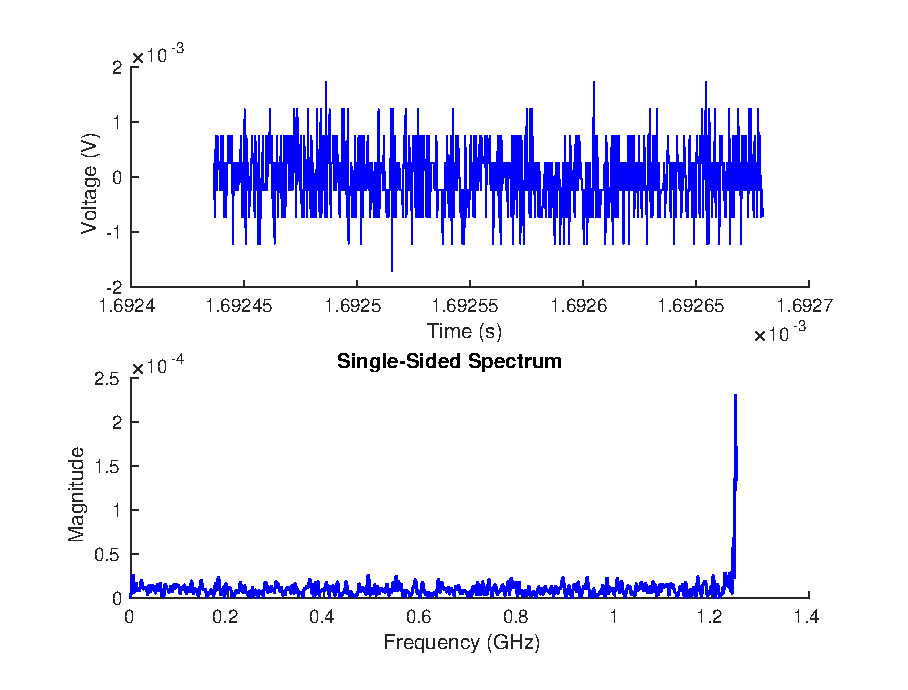
\includegraphics[width=.8\textwidth]{figures/chapter_background/Noise_white_sig_FFT_regWhiteNoise.eps}
\caption{White noise and its power spectrum}
\label{fig:backgrd_Noise_white}
\end{figure}
\begin{figure}[t!p]
\centering
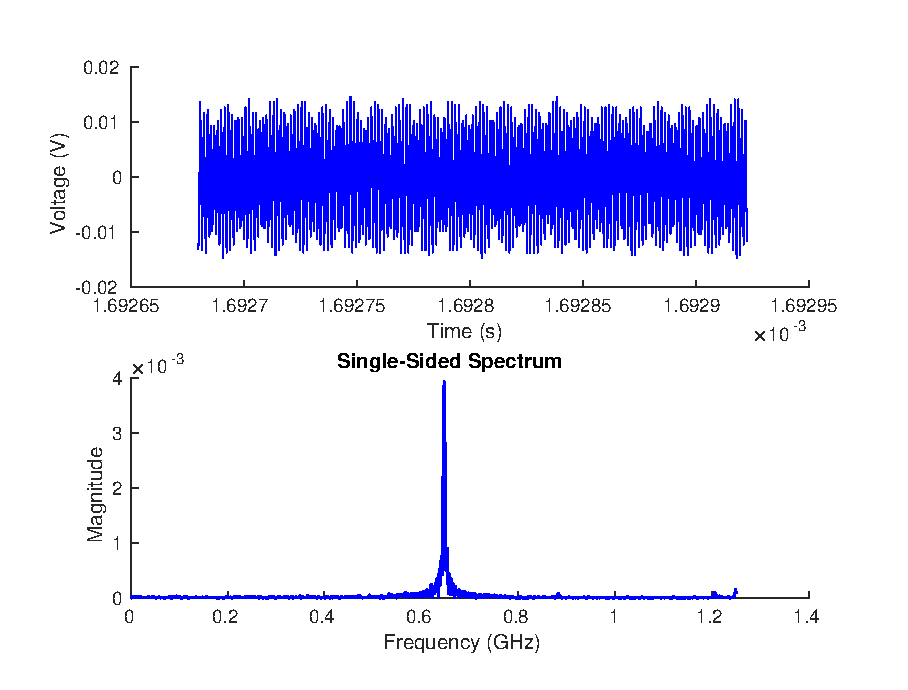
\includegraphics[width=.8\textwidth]{figures/chapter_background/Noise_freqStruct_sig_FFT_SineNoise2.eps}
\caption{Frequency-structured noise and its power spectrum.}
\label{fig:backgrd_Noise_frequency}
\end{figure}
\begin{figure}[t!p]
\centering
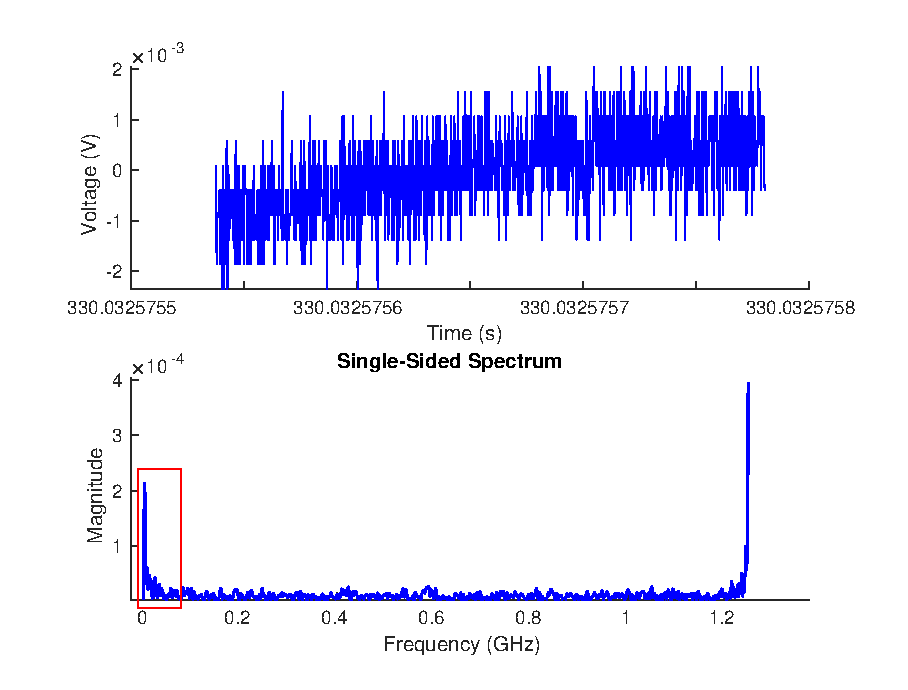
\includegraphics[width=.8\textwidth]{figures/chapter_background/Noise_timeStruct_sig_FFT_RampNoise.eps}
\caption{Time-structured noise. The noise in the red box is caused by the temporal-structured noise.}
\label{fig:backgrd_Noise_time}
\end{figure}

%%%%%
% Analog filter
%%%%%
\section{Filters}
In the application of laser rangefinder, the received laser pulse can be contaminated by all kinds of the noise mentioned above. The distortion of signals could result in uncertainty of the time measurement (Details will be described in Chapter~\ref{ch:TDC}, \ref{ch:ADC_BM} and \ref{ch:NP}). Therefore, the pulses need to be separated from the noise and should be restored if the signal is distorted. The noise removal can be achieved by filters. Filters have widely used in image processing, optics and electrical signal processing, and the filter referred to in this work is specifically for electrical signal processing. Generally, electrical filters can be classified as analog or digital filters. The simplest analog filters are RLC filters which are composed of capacitors, inductors and resistors, and other analog filters include crystal filters, microwave filters and mechanical filters \etc. The analog filters act on continuous-time (analog) signals, on the contrary, digital filters require an ADC to convert analog signals to digital samples, and processes digital signals by algorithms programmed in a digital signal processor (DSP). The section focuses on the fundamental concepts and characteristics of electrical filters but does not elaborate the details. Readers could refer to any textbook on signal processing for further information. The characteristics of electrical filters can be described in time and frequency domain. The characteristics in frequency domain is introduced first, followed by the time-domain characteristics.
% \todo{IIR and FIR? how do model }
\subsection{Frequency-domain Characteristics}
The characteristics in frequency domain of electrical filters can be described in time and frequency domain. sists of magnitude response and phase response. Figure~\ref{fig:Filter_freqResponse} presents a schematic of the frequency response of a low pass filter. The magnitude response describes the magnitude change (gain) by the filter at each frequency and the phase response presents the phase shift (or phase delay) at each frequency. The frequency response of a filter can be divided into three regions: \emph{passband}, \emph{transition band} and \emph{stopband}. The passband is the range of the frequencies passed by the filter, the stopband refers to the frequencies that are blocked, and the region in between is the transition band. According to the position of the passband at the frequency range, filters could be classified as low-pass (LP) filters, high-pass (HP) filters, band-pass (BP) filter, band-stop (BS) filters, and all-pass (AP) filters. The passband is bounded by a \emph{cutoff frequency}, $f_{cut}$, defined to be where the frequency magnitude response is reduced to -3 dB. In the passband, the frequencies are desired to be unaltered (flat passband or unity gain), but the gain may vary in certain filter designs and the fluctuation is called \emph{passband ripple}. Since large passband ripples alter the magnitude of in-band frequency components, the passband ripple should be remain small in a filter design. In the stopband, the blocked frequencies are attenuated by a \emph{stopband attenuation} which is measured between the peak of the passband magnitude and the largest stopband lobe magnitude. To sufficiently attenuate the stopband frequencies, the stopband attenuation should be adequately large. Note that filters usually have different gains at passband and stopband, but the all-pass filter, as indicated by the name, passes all the frequencies with a unity gain. It seems the all-pass filter has no change on the magnitude of the signal, but it plays an important role of modifying the phase of the signal which will be described in the next section. \par
The \emph{roll-off} of a filter is another important concept which defines the \emph{steepness} or slope of the magnitude response in the transition band, and it also sets the corn frequency of the stopband. A fast roll-off is preferred for a filter to truncate the undesired frequency band without affecting the rest spectrum, but the cost is the distortion of the frequency components at the passband. In other words, a steep transition band and a flat passband can not be achieve at the same time. Another key characteristic of a filter is the \emph{order}. The order of a filter is defined as the highest exponent in the numerator or denominator of the transfer function. The concept of the transfer function will not be expanded in this work, but in general, the order of a filter is equal to the number of delay elements in the filter structure, meaning that a filter of a large order offers a better magnitude response, but the large order also increases the complexity of the structure.
\begin{figure}[t!p]
\centering
\includegraphics[width=.8\textwidth]{figures/chapter_background/Filter_freqResponse.jpg}
\caption{Frequency response of a low pass filter: (a)Magnitude response (b) Phase response}
\label{fig:Filter_freqResponse}
\end{figure}
\subsection{Time-domain Characteristics}
In addition to the frequency-domain characteristics, the performance of a filter in time domain is also important, and the step response of a filter is a useful tool for the analysis of a filter in time domain. The time-domain parameters include the \emph{rise time} and \emph{overshoot} of the step response. The rise time of a filter describes the transition period of the step response, which should be short than the duration of a signal event (\eg changing from 'low' to 'high'), so that the event can be distinguished from the step response. Second, overshoot changes the magnitude of a signal, so it should be avoided when a filter is designed. Moreover, the phase response of a filter also plays a significant role in the time-domain characteristics of a filter. One of the key concept is the \emph{group delay} defined as
\begin{equation}\label{eq:backgrnd_AFE_groupDelay}
    \tau_g= -\frac{d\Phi(\omega)}{d\omega}
\end{equation}
where $\Phi(\omega)$ is the phase response at angular frequency $\omega$ and $\omega = 2\pi f$. The group delay is the slope of the phase response which depicts the linearity of the phase response. Here, the group delay should not be confused with the phase delay which is another key concept commonly used in the phase response. The phase delay is defined as following
\begin{equation}\label{eq:backgrnd_AFE_phaseDelay}
	\tau_{\Phi}= -\frac{\Phi(\omega)}{\omega}
\end{equation}
and it only describes the absolute phase shift at each frequency without any description of the relationship between the adjacent frequencies like the group delay does. Using Fourier transformation, a signal can be decomposed into several sinusoidal components with different frequencies. If a filter has a linear phase response, all the frequency components are delayed by the same phase, in which case all the components can still reconstruct the original signal shape, but only the time is shift. In this case, the phase delay is equal to the group delay. However, in the case of nonlinear phase response, the frequency components are shift by different amounts, so they can no longer compose the original signal shape, \ie the signal is distorted. If symmetric signals are used as in our case, the symmetry of the signal is impacted. Therefore, the linearity of the phase response is a powerful indicator of the distortion enforced by the filter, and a linear-phase filter is preferred for the applications that requires preservation of signal shapes. Additionally, the all-pass filter can also be used to alter the phase shift in this case. Even though the all-pass filter has no effect on the signal amplitude, it is designed to have different phase shifts among various frequencies, so that it can be placed after the other filters in the system to compensate the undesired phase shifts.\par
\subsection{Characteristics of different filters}
According to the characteristics of a filter in time and frequency domain, the filters can be designed in various types. The most common types of filter are Butterworth filter, Chebyshev filter, Elliptic filter and Bessel filter. The frequency response of the filters is shown in Figure~\ref{fig:Filter_freqResponse_diffType}. The magnitude response shows that both Butterworth and Bessel filter has no ripple at the passband, but the roll-off is slower than the other two. On the contrary, the Chebyshev and Elliptic filters sacrifice the flatness of the passband to achieve a faster roll-off, which is why they are commonly used for noise band removal. In the phase response, the Bessel filter has a maximally linear phase response, followed by the Butterworth filter having a a reasonable nonlinear phase response, while the phase response of the Chebyshev and Elliptic filters are very nonlinear. Therefore, the Bessel filter is the best option for the application where the shape of the filtered signal is crucial, and the shape distortion needs to be considered when the last two types of filter are selected. The application of the Butterworth, Chebyshev and Elliptic filters to different types of noise mentioned in Section~\ref{sec: noise} will be discussed in Chapter~\ref{ch:AFE}. 
\begin{figure}[t!p]
\centering
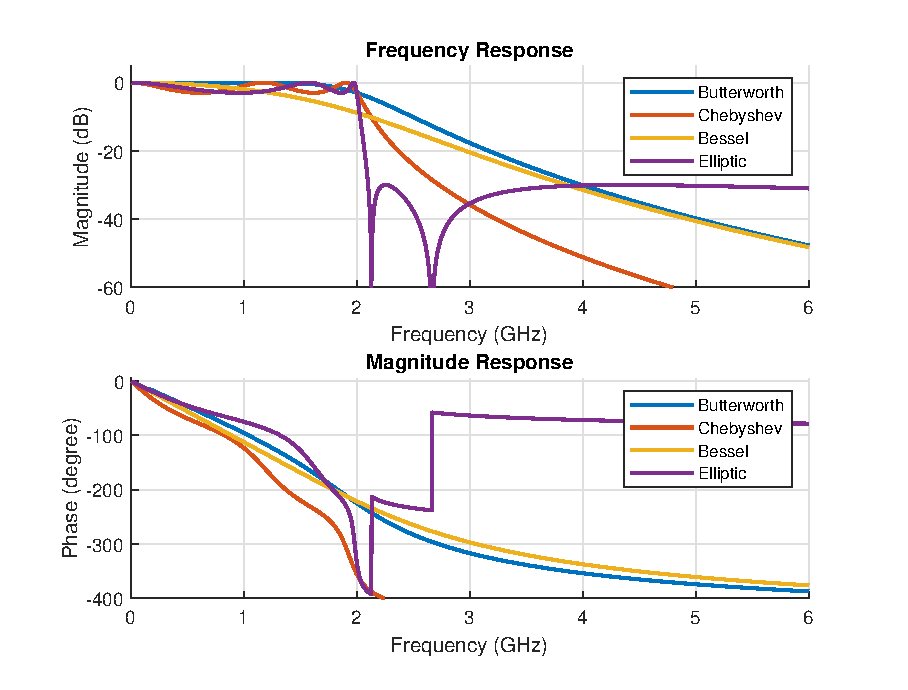
\includegraphics[width=.8\textwidth]{figures/chapter_background/Filter_FreqResp_diffFilters.eps}
\caption{Frequency response of different type of filters. The cutoff frequency is 2GHz, the order is 5, the passband ripple for the Chebyshev and Elliptic filter are 3 dB and the stopband ripple of the Elliptic filter is 30 dB.}
\label{fig:Filter_freqResponse_diffType}
\end{figure}
%%
% TDC
%%
\section{Time-to-Digital Converter}
After the photon detector converts returning laser pulses to analog signals, a time discriminator is required to measure the returning (stop) time of the signal. Given the transmitted (start) time of the pulse is measured beforehand, by calculating the time difference between the returning time and start time, the time-of-flight (TOF) of the emitted pulse and the corresponding distance of objects can be obtained. Generally, the start time and the returning time are usually discriminated by same techniques. Therefore, this section will only focus on the time discrimination techniques for the returning time, and the same principle is applied to the start time.\par 
Two approaches are commonly used for the time measurements. The first one is using a Time-to-Digital Converter (TDC), which consists of a comparator that generates logic signals by comparing input analog signals with a preset threshold, and a reference clock counter which measures the time when the logic signal changes its value from low to high. Both the start and stop time are measured in the same way. Then, the counter in the TDC subtracts the start time from the stop time to calculate the TOF. Different types of comparator and timing techniques will be described in the following sections, and Figure \ref{fig:TDC_schematic} presents a schematic of the TDC. The second approach is using an Analog-to-Digital Converter(ADC), which converts analog signals to digital signals. The ADC output is subsequently passed to a digital processor which performs numerical computation and extracts the time information of the signal. The TDC-based approach will be described next followed by the ADC-based techniques.\par
\begin{figure}[t!p]
\centering
\includegraphics[width=.8\textwidth]{figures/chapter3_TDC/schematic_TDC.jpg}
\caption{Schematic of TDC}
\label{fig:TDC_schematic}
\end{figure}
Various time discrimination methods are available for the TDC-based approach. Generally, the discrimination techniques fall into two main categories: leading-edge discrimination and constant fraction discrimination (CFD). In this section, the leading-edge discrimination techniques will be introduced first followed by the CFD techniques.\par
% leading edge detection
\subsection{Leading edge detection}
In the leading-edge discrimination, time is measured when the leading edge of a signal crosses a threshold set at the comparator. Since the measurement is carried out at the leading edge of a signal, the time detection will still be functional even the signal saturates photon detector. In other words, the leading-edge detection is not restrained by the dynamic range of the detector. \par
However, the major disadvantage of the leading-edge discrimination is that significant the walk error could be introduced due to the variation of amplitude of the signal. The walk error is illustrated in Figure \ref{fig:TDC_walkerror}. In Figure \ref{fig:TDC_walkerror}, the two signals are reflected by the same target but have different amplitudes. Keeping comparator thresholds and rise-times of the signals the same, the signal with a smaller amplitude crosses the threshold later than the larger pulse. The time shift due to the amplitude change is called walk error. The walk error is a major concern for the leading-edge detection, which could lead to significant timing inaccuracy. Therefore, many methods have been developed to compensate for the walk error.
\begin{figure}[t!p]
\centering
\includegraphics[width=.8\textwidth]{figures/chapter3_TDC/walk_error.jpg}
\caption{Illustration of walk error}
\label{fig:TDC_walkerror}
\end{figure}
%  insert TDC figure
\subsubsection{Gain-control compensation}
One way to reduce the walk error is to reduce the variation of signal amplitude by means of gain control. \cite{ruotsalainen2001wide} proposed a variable-gain amplifier followed by an amplitude-insensitive time discriminator. In the gain amplifier, the amplitude of a signal is first measured with a peak detector. Then, the attenuation of the gain control cells are adjusted accordingly to attenuate the amplitude of the signal to a constant value. Ideally, the gain-control technique allows a constant amplitude of a signal before entering the comparator. In practice, due to the limitation of the analog system, the achievable timing accuracy is $\pm 25 ps$ and the functional dynamic range is limited to $1:650$ \citep{ruotsalainen2001wide}. The limited operative range makes the gain-control less practical for the autonomous vehicle application, since the attenuation of the atmosphere and the reflectivity of the object can vary dramatically, which can result in a dynamic range of the amplitude of the signal of more than $1: 100,000$. 

\subsubsection{Time-over-Threshold (TOT) Compensation}
To allow a high dynamic range of input signals, the time-over-threshold(TOT) compensation and a slew-rate compensation were developed, \citep{kurtti2009pulse}, \citep{kurtti2011integrated} and \citep{nissinen2009integrated}. A schematic of the TOT compensation is shown in Figure \ref{fig:TDC_TOT}. In the TOT compensation, the crossing time at both leading edge and falling edge of a pulse are discriminated by the same comparator with the same threshold $Vth$. The time difference between the time marks at the leading and the falling edges is named the time-over-threshold (The time difference is named ‘pulse length’ in the original paper, but time-over-threshold is used here to avoid the confusion with the pulse width). As seen in Figure \ref{fig:TDC_TOT}, the TOT increases monotonically with the pulse amplitude and the walk error $\Delta_w$ decreases with the amplitude. Therefore, if the relation among the amplitude, walk error and the TOT can be found, the walk error can be determined and compensated by measuring the TOT.\par
\begin{figure}[t!p]
\centering
\includegraphics[width=.8\textwidth]{figures/chapter3_TDC/TOT.jpg}
\caption{Illustration of TOT compensation}
\label{fig:TDC_TOT}
\end{figure}
In practice, a look-up table or a compensation curve containing the relation of the walk error and the TOT is made by calibrating the TDC. It can be done by experimenting laser pulses with an amplitudes of a range of $1:100,000$, measuring the TOTs and walk errors for each amplitude, and calculating the corresponding ensemble average of TOT and walk error over the measurements. After the relation of the TOT and walk error is obtained, the walk error for a certain TOT can be found by extrapolating the compensation curve or the look-up table using the measured TOT value. Then, the walk error can be subtracted from the marked time at the leading edge of the signal to obtain the walk-error-free stop time. \citep{kurtti2009pulse} and \citep{kurtti2011integrated} proposed a compensation circuit to realize the TOT compensation. In this work, we provide the analytic relation among the TOT, pulse amplitude and walk error (The derivation is given in Appendix.): 
\begin{align}
    V_r&=\frac{V_{th}}{exp\big(\frac{(TOT/2)^2}{2\sigma^2}\big)}\\
    \Delta_w&=|t_{ref}|-\sqrt{t_{ref}^2-2\sigma^2\ln(\frac{V_{ref}}{V_r})}
\end{align}
where $V_{th}$ is the threshold, $V_r$ is the amplitude of a returning signal, sigma is the standard deviation of the signal, $t_{ref}$ and $V_{ref}$ are the convenient reference amplitude and time for calculation of walk error $\Delta_w$, and TOT is the measured TOT value. The relations between amplitude and TOT, amplitude and walk, and TOT and amplitude are presented in Figure \ref{fig:TDC_TOTcurve}. We also provide an analytic model of the TOT compensation process taking the TOT measurement as input and using the above relations. A schematic of the compensation process is shown in Figure \ref{fig:TDC_TOTcurve} (c).\par
The TOT method can achieve a time measurement precision of picosecond level and is operative in a larger dynamic range of the signal amplitude of $1: 30,000$ \citep{Kurtti2009PulseRangefinder}. However, we should notice that the TOT method is highly sensitive to the symmetricity of the signal. In other words, if the falling edge of the signal is heavily distorted due to, for example, multiple returns or amplification noise of the TIA, the relation between the TOT and the walk error is impaired. In this case, the TOT compensation will not be useful. 
\begin{figure}[t!p]
\centering
\includegraphics[width=1\textwidth]{figures/chapter3_TDC/TOT_curve.jpg}
\caption{TOT compensation curve}
\label{fig:TDC_TOTcurve}
\end{figure}
% slew rate
\subsubsection{Slew-rate Compensation}
An alternative way to compensate the walk error is to use the relation of the walk error and the slew rate of the return pulse, which is called slew-rate compensation. The slew rate is the slope of a signal at the point of interest. For the slew-rate compensation, the TDC is equipped with two comparators with two preset thresholds. A schematic of the slew-rate compensation is shown in Figure \ref{fig:TDC_slewrateLinear}\todo{change figure to sufigure and caption}. The lower threshold ($V_{th1}$) is set as normal in a TDC, and the higher threshold ($V_{th2}$) is set certain times larger than Vth1, i.e. $V_{th2} = CV_{th1}$. Two timestamps, t1 and t2 are measured from the comparator with respect to $V_{th1}$ and $V_{th2}$, and the time difference between $t_1$ and $t_2$, $\Delta_t$, is calculated. The walk error $\Delta_w$ is the time difference between $t_1$ and a convenient time reference $t_{ref}$. If the portions of the signal below the high threshold have a linear slew rate as shown in Figure \ref{fig:TDC_slewrate}, the walk error has a linear relation with the $\Delta_t$ \citep{nissinen2009integrated}:
\begin{align}
    \Delta_w=\frac{\Delta_t}{C-1}
\end{align}
\begin{figure}[t!p]
\centering
\includegraphics[width=.8\textwidth]{figures/chapter3_TDC/slew-rate.jpg}
\caption{Illustration of slew-rate compensation(linear)}
\label{fig:TDC_slewrateLinear}
\end{figure}
\begin{figure}[t!p]
\centering
\includegraphics[width=.8\textwidth]{figures/chapter3_TDC/slew-rate0.jpg}
\caption{Illustration of nonlinear slew-rate compensation}
\label{fig:TDC_slewrate}
\end{figure}
However, a Gaussian signal usually has a nonlinear slew rate at the bottom, which results in a nonlinear dependency of the walk error on the time difference. Therefore, the dependency can be either obtained by calibrating the TDC like the TOT compensation or derived mathematically. For the calibration of the compensation curve or the look-up table, the walk errors and dts are first measured and calculated from signals with a wide range of amplitude, then, the averaged walk error and time difference is calculated for each amplitude. Consequently, the walk error can be obtained by extrapolating the compensation curve or the look-up table for a measured time difference, and the walk error is subtracted from the first stop time to remove the walk error on the return time.\par
In this work, we mathematically derived the nonlinear relation of walk error and time difference, and provide an analytical compensation model using MATLAB. The relationship is given as following and the derivation is detailed in Appendix. The relation between the walk error and the dt is plotted in Figure \ref{fig:TDC_slewrate_curve}.
\begin{align}
    \Delta_t&=STOP_2-STOP_1\\
    \Delta_w&=\frac{-2\sigma^2\ln(C)-\Delta_t}{2\Delta_t}-t_{ref}
\end{align}
\begin{figure}[t!p]
\centering
\includegraphics[width=1\textwidth]{figures/chapter3_TDC/slew-rate_curve.jpg}
\caption{Slew-rate compensation curve}
\label{fig:TDC_slewrate_curve}
\end{figure}
The slew-rate compensation can also achieve picosecond-level precision in large dynamic range as demonstrated by Nissinen. In addition, its independence on the falling edge of the signal makes it more applicable than the TOT compensation, but the additional comparator for the time difference measurement increases the complexity of the discriminator. \par
The TOT and slew-rate compensation significantly reduce the walk error, but also introduce additional noise to timing results. One example is the quantization error due to the utilization of extrapolation on the compensation curves, and the number of points used in the extrapolation affects the significance of the quantization error. In addition to the error induced by the compensation, the TDC-based timing techniques have their own inherent noises, of which jitter is an important one. Jitter is the uncertainty on measuring the time when a signal crosses the comparator threshold. If the signal is noise-free, the jitter on the time measurement is zero. However, in practice, amplitude variation always exists due to unavoidable electrical noises, in which case, the leading-edge detection produces time results with jitter errors. The jitter is defined mathematically as following \citep{skolnik1962introduction}:
\begin{align} \label{eq:TDC_jitter}
    \sigma^2_{jitter}=\frac{\sigma^2_{noise}}{(dV/dt)^2}=\frac{t^2_r}{SNR^2}
\end{align}
from which, we can see its inverse relationship with the slew rate at the trigger position.\par
In the above leading-edge discrimination methods, constant thresholds set at a certain level above the noise floor are used. Even though those trigger positions have less electrical noise compared to the higher portion of the pulse (shot noise increases with signal amplitude), the slew rate at those positions is smaller. According to the Equation \eqref{eq:TDC_jitter}, small slew rates leads to large jitter. Ideally, the trigger position should be at the linear portion ($30\%$ - $40\%$) of the amplitude of a pulse) of the leading or falling edge of a pulse \citep{kilpela1998timing}, where the signal has a sharp slew rate. In practice, keeping the threshold adjustable at a constant fraction of a pulse will minimize the jitter. However, the abovementioned ‘constant-threshold’ method makes the adjustment of the trigger position impossible.
% time variant thresholding
\subsubsection{Time-variant thresholding}
Since the constant threshold could increase timing jitter, a time-variant threshold method was proposed by [http://voxtel-inc.com/files/ROX-InGaAs-APD-Photoreceivers.pdf]\todo{change citation}, which adaptively adjusts the threshold according to the time elapsed from the start time of a pulse. In this case, the threshold-crossing time can be kept around the optimal trigger position. The relation of the time-variant threshold and the time elapse is given by: 
\begin{equation}\label{eq:TDC_time1}
    V_{th}(t)=V_{th,lo}+(V_{th,hi}-V_{th,lo})e^{-\frac{t}{RC}}
\end{equation}
where $V_{th, hi}$ and $V_{th}$, lo are predefined optimal thresholds for short and long-distance object, respectively. In the work, $V_{th, hi}$ is set at $30\%$ of the amplitude of the returning pulse from a 10m-away object, with a reflectivity of $10\%$ and visibility of 10km. $V_{th}$, lo is set above six times the noise floor of a signal from a 200m-away object, keeping other conditions the same as for $V_{th, hi}$. The $R$ and $C$ are the resistance and capacitor values, which compose of the time constant that approximates the $1/R^2$ power attenuation as a function of range. Note that the dependency of power attenuation on object distance should follow the lidar equation, simplified as: 
\begin{equation}\label{eq:TDC_time2}
    V_r=\frac{V_0A}{R^2}e^{-2BR}
\end{equation}
where $R$ is the object distance, $A$ and $B$ are parameters, and $V_0$ and $V_r$ are the peak voltage of the transmitted and returning signal, respectively. Comparing Equation \eqref{eq:TDC_time1} and Equation \eqref{eq:TDC_time2}, we can see Equation Equation \eqref{eq:TDC_time1} can not exactly model the function of power attenuation of range, which results in variations of the trigger position around the optimal position. Moreover, the time constant, $R$ and $C$, requires careful calibration to match the Lidar equation in practice.\par
The time-variant provides a solution to the trigger positioning issue to reduce timing jitter, but the walk error remains unsolved. Therefore, the TOT compensation was combined with the time-variant threshold method in [http://voxtel-inc.com/files/ROX-InGaAs-APD-Photoreceivers.pdf]\todo{change citation}. However, the TOT compensation restrains the method to symmetrical laser pulses. In this work, both the TOT compensation and the slew-rate compensation are combined with the time-variant threshold method in the time discrimination model.
%CFD
\subsection{Constant Fraction Discrimination (CFD)}
\subsubsection{ Traditional CFD}
In addition to the time-variant threshold method, the Constant Fraction Discrimination or CFD techniques, as illustrated as the name, can also trigger the time at a constant fraction of a pulse height. For the traditional CFD, the input signal is divided into two parts, one of which is attenuated and inverted, and the other one is delayed. The schematic of the CFD is shown in Figure \ref{fig:TDC_cfd} and Figure \ref{fig:TDC_cfdcircuit}. The attenuation is selected as a fraction of the original pulse amplitude, at which the timing position is optimal, and a value between $20\%$ and $40\%$ is a reasonable choice. The time delay is then tuned to make the fraction point on the leading edge of the delayed signal aligned with the peak of the attenuated pulse. Subsequently, the two signals are added to generate a bipolar signal, which is then passed to a zero-crossing comparator to generate the logic signal for time discrimination. The zero-crossing point corresponds to the time at the optimal fraction point on the delayed signal, which is also the time at the peak of the original signal. In addition, a leading-edge arming discriminator triggered above the noise floor of the signal is added, to prevent the zero-crossing comparator from being mistakenly triggered on noise floor preceding the zero-crossing point.\par
\begin{figure}[t!p]
\centering
\includegraphics[width=.8\textwidth]{figures/chapter3_TDC/cfd.jpg}
\caption{Schematic of the principle of CFD algorithm}
\label{fig:TDC_cfd}
\end{figure}
\begin{figure}[t!p]
\centering
\includegraphics[width=.8\textwidth]{figures/chapter3_TDC/cfd_circuit.jpg}
\caption{Schematic of a CFD circuit}
\label{fig:TDC_cfdcircuit}
\end{figure}
The major advantage of the CFD is that it theoretically eliminates the walk error due to the independence of the zero-crossing point on pulse amplitude as shown in Figure \ref{fig:cfd_zerocrossing}. However, in practice, a finite amount of charge is required to move the comparator output from “0” to “1”, which results in additional walk error on the timing results\citep{nakhostin2017signal}. Additionally, since the summation is carried out at the peak of the signal, the traditional CFD also suffers from the saturation of the APD or multiple returns from a transmitted pulse. In other words, if the incoming signal has strong amplitude beyond the dynamic range of the photon detector which saturates the detector, or multiple returns come back in a minuscule time difference, the top of the pulse is flattened. The flattop could result in large walk error on timing results, which is why the traditional CFD is normally used in a limited range of 1:100 or less for the input signal\citep{kurtti2011integrated}\par
%, and the use of CFD less than 100: [12] [15] [26] – check ref.]}\par
\begin{figure}[t!p]
\centering
\includegraphics[width=.8\textwidth]{figures/chapter3_TDC/cfd_zerocrossing.jpg}
\caption{Independence of the zero-crossing point on signal amplitude}
\label{fig:cfd_zerocrossing}
\end{figure}
In addition to reducing the walk error, the CFD also often results in less time jitter. In principle, in the summation process of the CFD, the noises of the attenuated and the delayed signals are added as well, which should result in an increase of the variance of the noise on the bipolar signal by a factor of $1+f^2$:
$$
\sigma_{CFD}^2=(1+f^2)\sigma^2
$$
where $f$ is the CFD attenuation factor, $\sigma^2$ is the variance of the original signal, and uncorrelated noise condition is assumed [https://www.ortec-online.com/-/media/ametekortec/application\%20notes/an42.pdf]\todo{change citation}. According to Equation \eqref{eq:TDC_jitter}, the jitter for the CFD is worse compared to the leading-edge detection (of which the noise variance is sigma). However, the CFD virtually reduces the jitter, because the statistical variation of the noise on the attenuated and the delayed signals cancel out each other and consequently, the jitter is mitigated. Moreover, since only the leading edge and the peak of the signal are involved in the summation, the CFD is not limited by the pulse symmetricity. 
\subsubsection{Leading-falling edge CFD}
Noticing the limitation by involving the peak of signals, a variation of the traditional CFD, leading-falling edge CFD was developed to avoid this issue. The principle of the leading-falling edge CFD is similar to the traditional CFD as shown in Figure \ref{fig:cfd_leadFall}, which divides the original signal to two identical signals. But the rest steps are different: no signal is attenuated, but one of the signals is delayed by a certain amount, such that the leading edge of the delayed pulse and the falling edge of the non-delayed pulse cross at the optimal constant fraction of the signal height. In this case, the two signals are intersected at rather than the peak but a fraction point which has the largest slew rate of the signal. The leading-fall edge CFD can prevent the detection suffering from the flattops, but since the technique involves the falling edge of the signal, it is only practical for symmetric pulses. 
\begin{figure}[t!p]
\centering
\includegraphics[width=.8\textwidth]{figures/chapter3_TDC/cfd_leadFall.jpg}
\caption{Principle of leading-falling edge CFD}
\label{fig:cfd_leadFall}
\end{figure}
\subsection{Summary}
From the comparison of the leading-edge and CFD detection, we can see that leading-edge detections have a simpler circuit design than the CFD techniques which need delay and summation circuits, but the walk error is a major drawback for the leading-edge discrimination techniques. Therefore, additional compensation techniques that are operative in a large dynamic range are required to achieve high timing accuracy. On the other hand, the CFD techniques provide a solution to significantly address the walk error and jitter, but potential time delay could result from the extra electrical components. The limited operative range of the CFD techniques also restrains their application in the automotive industry.
%%
% ADC
%%
\section{ADC-based Time Discrimination}
% Trigger Modes edge and level triggers 
\subsection{Digital Processing}
The ADC-based time discrimination is using ADC to convert analog signals output from a detector to digital signals, and measure the time of the digital returning pulse. The structure of the ADC-based discriminator is shown in Figure \ref{fig:schematic_ADC}.\par 
The digitization process of an ADC consists of two steps: sampling and quantization. The sampling step is to sample the analog signal in time by a sample-and-hold device that takes and holds a value from the continuous signal every $T_s$ second. The time interval $T_s$ is called the sampling interval and the sampling rate is denoted as $f_s$ = $1/T_s$. The resultant signal has a discrete time sequence but still continuous values for amplitude. In the quantization step, the continuous amplitude is converted to discrete values by a quantizer, and subsequently, a signal with discrete values in both time and amplitude, the so-called digital signal, is generated and output from the ADC.
\begin{figure}
\centering
\includegraphics[width=.8\textwidth]{figures/chapter3_TDC/ADC_schematic.jpg}
\caption{Schematic of ADC}
\label{fig:schematic_ADC}
\end{figure}
\subsection{Quantization}
In the quantization process, an important parameter of the quantizer is the resolution, which indicates the number of discrete values (quantization levels) it can produce over the dynamic range of the signal amplitude. The resolution is usually expressed in bits. For example, for a 6 bits ADC, there are $2^6$ discrete values or levels to store the signal amplitude. The difference between two successive quantization levels is called quantization steps \citep{nakhostin2017signal}
\begin{align}
\Delta = V_{k+1} – V_k 
\end{align}
Thus, the quantization steps Delta and the ADC resolution B, are related to the range R of the input signal:
\begin{align}
R=2^B\Delta    
\end{align}
As seen above, the nature of the quantization process is to approximate the continuous signal by discrete values. Thus, the finite number of quantization levels introduces error between the digital signal and the original analog signal. The error is denoted as the quantization error, and it is a function of the quantization step:
\begin{align} \label{eq:ADC_quanError}
\delta^2=\frac{\Delta^2}{12}     
\end{align}
where sigma is the standard deviation of the quantization error. The signal-to-quantization noise ratio  defined as the ratio of the signal power to the noise power, can be written in dB as \citep{nakhostin2017signal}
\begin{align} \label{eq:ADC_snrDB}
SNR_{dB} = 6.02B + 1.76    
\end{align}. It should be noticed that an ADC with high resolution would have less quantization error and a large signal SQNR.
\subsection{Sampling and aliasing}
The sampling rate of the ADC also affects the reconstruction of the analog signal. As known from the Nyquist’s theorem, the sampling rate should be equal to or larger than twice the largest frequency (Nyquist frequency) of the signal to correctly represent the signal, i.e.$ f_s \geqslant 2f_{max}$. Otherwise, aliasing occurs. However, it is not always possible to precisely measure the bandwidth of the input signal of the ADC, so the Nyquist criterion may not be met in practice. Therefore, to prevent aliasing, a low-pass filter is usually placed before the ADC (the AFE shown in Figure 10), to remove or attenuate the frequency components larger than the Nyquist frequency, and such filter is called anti-aliasing filter. In many cases, the anti-aliasing filter cannot completely remove all the high-frequency components due to the transition band of the analog filter. Therefore, to minimize the aliasing, an anti-aliasing filter could be designed to attenuate the frequency higher than the Nyquist frequency to a degree less than the quantization error\citep{mitra2006digital}. This could be achieved by selecting a filter with a sharp transition band or sacrificing some in-band frequencies by moving the transition band inside the bandwidth. However, either sharp transition band or cutting off in-band frequencies could cause distortion of the original signal. Alternatively, oversampling of the signal to a rate much higher than the Nyquist frequency is also often used to simplify the anti-aliasing filter and reduce the aliasing error.
\subsection{Functionality of an ADC}
Important functionality of an AD is introduced next, and the first one is the ADC mode. An ADC usually has multiple channels taking analog inputs, and the channels share one ore more that one clocks. The ADC mode is the combination of the channels that can be used. Taking a 4-channel ADC (Channel A, B, C, D) with a clock (5GHz) as an example, the ADC can be operated in 1-channel(Channel A, B, C, D), 2-channel(\eg AC, BD, \etc) and 4-channel mode(\eg AAAA, ABCD, \etc). Since all the channels share one clock, 4-channel mode has sampling frequency of 1.25GHz signal, one forth of the speed of 1-channel mode (5GHz). In the application of TOF estimation, the 2-channel mode is used which takes the analog signals from the laser source (START signal) and the photon-detector(STOP signal) as the inputs. Another feature of an ADC is the analog offset. Using the analog offset function, users can remove the DC of the signal to maintain the signal in the middle of the ADC range, which maximizes the dynamic range.\par
The zero-suppression function is also important for an ADC to reduce the load of data transfer. The zero suppression means only the ADC only start to acquire data when the predefined ADC threshold are exceed, and the stored waveform data is referred as 'packets'. A packet contains the sampled data and the absolute time of the last sample of the packet, and the absolute time is measured since the data acquisition start. Additionally, the ADC can also save a number of samples before the ADC trigger point, which is call precursor. The timestamp of each sample of a signal have to be calculated using the time interval between the successive samples and the number of samples. Moreover, the zero suppression function have two trigger modes: edge-triggering and level triggering, which collect data in two different ways. The two trigger modes acquire data in the unit of bin, which is a group of 8 points for 2-channel mode. The edge-trigger mode specifies the length of the precursor in bins and the number of bins after the ADC trigger point (collection length), which means all the data collected under the edge-trigger mode has the same length, but not all the samples are guaranteed to be above the threshold . On the contrary, the level-trigger mode saves all the samples above the threshold instead of saving a fixed number of samples, which means the length of the stored data is dependent on the signal. In addition, the level-trigger mode can not only save samples before the trigger point, but also save samples after the point becomes lower than the threshold, which is call post-cursor. The edge and level trigger mode are illustrated in Figure~\ref{fig:ADC_edge} and Figure~\ref{fig:ADC_level} \todo{change schematic of level and edge trigger, add label of precursor and post cursor, change the context using after-cursor to postcursor}
\begin{figure}[t!p]
\centering
\includegraphics[width=1\textwidth]{figures/chapter_background/ADC_edge.jpg}
\caption{Edge-trigger mode}
\label{fig:ADC_edge}
\end{figure}
 
\begin{figure}[t!p] 
\centering
\includegraphics[width=1\textwidth]{figures/chapter_background/ADC_level.jpg}
\caption{Level-trigger mode}
\label{fig:ADC_level}
\end{figure}
 
\include{chapter_Experimental_Setup}
\chapter{Physics-based Lidar Simulation - Transmitted Pulse}
A generic laser system consists of laser sources, optics, scanners(scanning lidar) or emitters(flash lidar), photon-detectors, timing devices, and a propagation medium as as air. The proposed physics-based full-system lidar simulator covers all the major components of a lidar system. 
%%%%%%%%%%%%%%%
%% 1. Laser Source
%%%%%%%%%%%%%%%

%% pulse model
\section{Transmitted pulse model}
In this work, the laser pulse is assumed to have a Gaussian distribution in time ~\citep{richmond2010direct,Budge2006SimulationLadarSIM}:
\begin{equation}  \label{eq:GauModel}
P_t(t) =\frac{E}{\sigma \sqrt{2\pi}}e^{-\frac{-t^2}{2\sigma^2}}
\end{equation}
where $E$ is the pulse energy of the laser, and $\sigma$ is the standard deviation of the Gaussian distribution. The relation between the standard deviation, the pulse width $\Delta t_w$ and the rise time $\Delta t_r$ are
\begin{equation} \label{eq:FWHM}
\Delta t_w=2\sigma\sqrt{2\ln2}\approx2.355\sigma
\end{equation}
\begin{equation} \label{eq:rt}
\Delta t_r\approx1.687\sigma
\end{equation}
assuming the area under the Gaussian curve is equal the area of a rectangular defined by the pulse width and the peak power. The derivation is given \todo{add appendix}. The peak power can be found as
\begin{equation} \label{eq:peakpower}
P_0 = \frac{E}{\Delta t_w} =\frac{E}{2\sigma\sqrt{2\ln2}}    
\end{equation}
Inserting Equation \eqref{eq:FWHM} and \eqref{eq:peakpower} to Equation \eqref{eq:GauModel}, the Gaussian pulse model used in this work is obtained
\begin{equation}\label{eq:pulsemodel}
P_t(t)=2\sqrt{\frac{\ln2}{\pi}}P_0e^{-4\ln2\frac{t^2}{\Delta t_w^2}}\approx0.94P_0e^{-4\ln2\frac{t^2}{\Delta t_w^2}}.
\end{equation}
Equation \eqref{eq:pulsemodel} also describes the relation between the height of the Gaussian pulse and the peak power: $h_{pulse}\approx0.94P_0$. Using Equation \eqref{eq:pulsemodel}, one can obtain the temporal power distribution of the transmitted pulse given the peak power, the pulse width of a laser source and a time sequence. The corresponding pulse energy, average power, and rise time can also be obtained using the equations above. However, one should note that a shortcoming of the model is that the model gives a non-zero signal power even for the time before the laser is fired ($t<0$), which causes a violation of causality.\todo{add pulse figure}

%% results and validation
\section{Results and Validation}
In this study, the parameter of the prototype lidar was utilized in the pulse model, and is given in \todo{chapter exp}. The pulse model was then validated by converting the modeled pulse in power to voltage and comparing with the start signal measured from the prototype lidar using an oscilloscope. The experimental setup for the validation is given in \todo{figure} and \todo{change number} 493 observations of the start signal were measured in voltage. The rise time, pulse width, and the height of the pulse generated by the pulse model and measured in the experiment were calculated. One example of the measured transmitted pulse is shown in Fig.~\ref{fig:pulse} along with the modeled pulse. The parameters of the laser were compared and shown in Table~\ref{table:param_pulseModel}. For the parameter of height of pulse, the bold value represent the original measured or modeled heights, while the other one is the corresponding value after the conversion between voltage and power.
\begin{figure}[htbp] % position options
\centering
\graphicspath{ {figures/} }
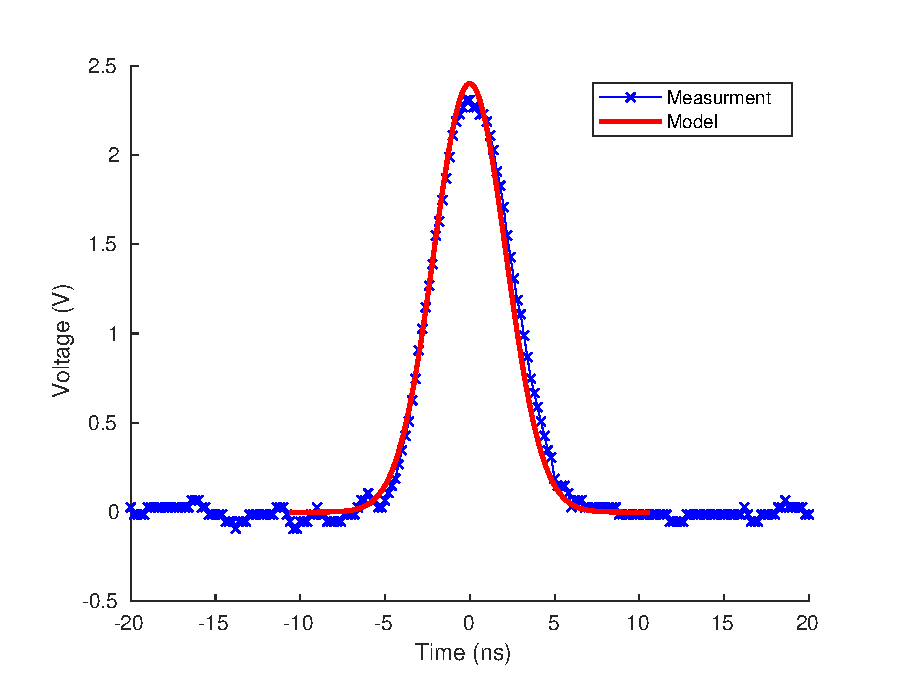
\includegraphics[width=0.8\textwidth]{figures/chapter4_pulse/Fig_pulse_model_meas.eps}
\caption{Example of pulse model}
\label{fig:pulse}
\end{figure}

\begin{table}[htbp]
\caption{{Parameters of Transmitted Pulse}}
\centering
\label{table:param_pulseModel}
\begin{tabular}{|l|l|l|l|}
\hline
Parameters    & Measurement & Model\\ \hline
Height of pulse (V) & $\mathbf{2.407\pm 0.107}$ &  $2.399$             \\ \hline
Height of pulse (W) & $558.04\pm 24.8$ &  $\mathbf{556.1}$             \\ \hline
Rise time (ns) & $3.119\pm0.413$ &  3.52   \\ \hline
Pulse width (ns) & $5.85 \pm0.318$ &  5  \\ \hline
\end{tabular}%
\end{table}

% sampling rate

% \subsection{Sampling rate}
% In the pulse model, we are using digital values to simulate continuous lase pulses, which requires a sufficient high sampling rate of the digital signal, so that (1) no aliasing occurs and the pulse shape is well represented, and (2) the natural of finite time intervals has minimum effects on the accuracy of distance measurements. However, on the other hand, if the sampling rate is too high, no additional information is provided and the computational cost is increased. Therefore, we studied the effect of different sampling rates on the distance measurement next and provide sduggestions on the selection of a proper sampling rate that balances the requirements and the computational cost.
\section{Sampling Rate}
1. in the previous result we have not talked about samplign rate. 
The sampling rate is another variable that needs to be considered, since
we use discret signal to simulate continous analog signal

wahab summaried the discussion of samplign rate of signal for chrom....and suggest (last sentense).
The response time or RC time constant is  an important factor for the sampling rate decision for lidar simualtion as well, in additino to other factors: timing device resoluion... 
Therefore, we listed the factors that need to be considered for the lidar simulation:

% 2. to be considered:
(1) represent signal well
-signal bw
(2) no effect on timing accuracy
(3) no effect on timing resolution
(4) represent noise and effect of noise on measurement well
-white noise ->  infinite high frequency, but the signal need to be process by a circuits => so we also have to consider prop delay
(5) computational cost

To decide a sampling rate for this study corresponding to the devic3 parameters, we performed tests on several different srs, and the check if the metris are meet. and chose the lowest one  meeting all the metrieis for lowest computational cost.
\subsection{Experiments}














% %%%%%%%%%%%%%%%
% %% Timing Module
% %%%%%%%%%%%%%%%

% \section{Time Discriminators}
% \subsection{Time-to-digital converter approaches}
% \subsection{Analog-to-digital converter approaches}

% \subsubsection{Digital version of the analog timing techniques}
% After an ADC converts analog signals to digital signals, different timing techniques are applied on a DSP to determine the time of the returning pulse. One approach is implementing a digital version of the analog timing techniques, i.e. leading-edge detection techniques or CFDs. The details of those methods are described in above sections and are skipped here, but it should be noticed that for the digital signals, the threshold generally does not coincide to the sample points of the signal. Therefore, interpolation between neighborhood samples is needed to find the exact time mark corresponding to the threshold value. Linear interpolation is a common selection, but the interpolation could affect the timing accuracy, depending on the local linearity of the signal. More specifically, if the curvature of a signal in the proximity of the threshold is large (the pulse has a nonlinear shape), time walk could occur. Note that this walk error is different than the walk error mentioned in the TDC-based approaches. The effect of the curvature is illustrated in Fig \textcolor{yellow}{(Fig10.27 Mahammad book). }

% \subsubsection{Detector and Estimator}
% The digital version of the analog timing techniques that utilize the ADC as a TDC limits the potential of the ADC, since the information contained in the digital signal is valuable for the improvement of the accuracy of signal detection and estimation. Therefore, time discrimination algorithms taking advantage of the shape information is illustrated next, which are generally composed of a detector and an estimator following a ADC. The function of the detector is to determine the presence or absence of a predefined signal from a signal contaminated by noise. In our case, if a Gaussian pulse with certain characteristics (\ie rise time, pulse width, \etc) is present in the returning signal. If the pulse is present, an estimator is needed to estimate the values of the parameters of the signal (arrival time of the pulse in our case) by mathematically modeling the signal. \\
% In this work, determining the presence of a pulse is performing a binary hypothesis test $\mathcal{H}_1$: pulse or $\mathcal{H}_0$: noise, and \cite{kay1998fundamentals} recommended using a Neyman-Pearson(NP) detector or Bayesian approaches for such a problem. Bayesian approaches require a prior knowledge of the likelihood of the hypotheses, or \emph{prior probabilities}: $P(\mathcal{H}_1)$ and $P(\mathcal{H}_0)$ , but it is usually not available for radar or lidar applications, neither for this work. Thus, the NP detector is considered in this study. The NP detector has been proven to be the optimal detector for radar/ laser signal detection\cite{kay1998fundamentals}, and has been widely utilized in many applications like target detection, medicine, nuclear energy, gravitational-wave astronomy, \etc\cite{Hoover2000LocatingResponse,Bousselham2007SamplingTiming,seto2001possibility,gronwall2007influence,gu2002detecting,Jordan2009RangeData,roman2000parametric,Ofek2017OptimalDetection,Vio2018MatchedImplementation}. In general, the NP detector conducts a likelihood ratio test(LRT\textcolor{yellow}{equation..}) for detection of a known deterministic pulse, \ie the pulse has no unknown parameters, while in our case some parameters of the pulses are unknown,\eg the arrival time (the amplitude of the pulse is less important). Therefore, a more general LRT(\emph{generalized likelihood ratio test}, or GLRT) is used for such situation, by using which the parameters of the pulse (arrival time) will be determined simultaneously. Consequently, our problem that the detecting the returning pulse and estimating the arrival time are combined to a single problem, and it can be solved by applying a NP detector with GLRT. The principle of the NP detector, LRT and GLRT will be introduced next followed by the application of the detection theories to solve our problem.

% \subsubsection{Neyman-Pearson Detector}
% \paragraph{Problem definition}
% First, we need to define our problem mathematically, that is,  to distinguish between the hypotheses $\mathcal{H}_1$: pulse or $\mathcal{H}_0$: noise:
% \begin{align}\label{eq: hy}
% \mathcal{H}_0:x[n]&=w[n]  &n=0, 1,\ldots, N-1\\
% \mathcal{H}_1:x[n]&=s[n-n_0]+w[n]  &n=0, 1,\ldots, N-1    
% \end{align}
% where $x$ is the returning digital signal,  $w$ is the noise following a Poisson distribution with the expected value $E[w]=W$, and $W$ is the mean of the total noise current which is the summation of the mean dark current $D$ and mean background current $B$, \ie $W = D + B$ , and $w\sim Pois(W)$. $s$ is our transmitted pulse that is deterministic and nonzero over the time interval $[0, M-1]$.  $n$ stands for each data point in the digital signal which is bounded by the observation time period $[0, N-1]$, and $n_0$ is the arrival time of the pulse, $n_0\in[0, N-M]$. Our goal is to decide the hypothesis a returning signal should fall with a certain false alarm rate $P_{fa}$, and if it is a pulse, we need to estimate the value of $n_0$.
% \paragraph*{Neyman-Pearson Theorem}
% The Neyman-Pearson theorem allows us to design a detector to achieve our goal: to maximize the detection probability $P_D$ for a given $P_{fa}  =\alpha$, decide $\mathcal{H}_1$ if the generalized likelihood ratio $L_G(x)$ is greater than a threshold $\gamma$; otherwise, decide $\mathcal{H}_0$: \textcolor{red}{need to talk about $\hat{n}_0$}
% \begin{equation} \label{eq:Lx}
% L_G(x)=\frac{p(x;\hat{n}_0,\mathcal{H}_1)}{p(x;\mathcal{H}_0)}\underset{\mathcal{H}_0}{\overset{\mathcal{H}_1}{\gtrless}}\gamma
% \end{equation}
% where the threshold $\gamma$ is found from
% \begin{equation}\label{eq:pfa}
% P_{fa}=\int_{\{x:L_G(x)>\gamma\}} p(x;\mathcal{H}_0)dx=\alpha
% \end{equation}
% And the detection probability $P_D$ is defined as
% \begin{equation} \label{eq:pd}
% P_D=\int_{\{x:L_G(x)>\gamma\}}p(x;\hat{n}_0, \mathcal{H}_1)dx
% \end{equation}
% The generalized likelihood ratio $L_G(x)$ indicates the likelihood of $\mathcal{H}_1$ versus the likelihood of $\mathcal{H}_0$, and the Equation \eqref{eq:Lx} is called the generalized likelihood ratio test (GLRT). The 'generalized' indicates the signal has unknown parameters. The probability density distribution (PDF) $p(x;\hat{n}_0,\mathcal{H}_1)$ stands for the PDF of the signal with an unknown parameter $\hat{n}_0$ under $\mathcal{H}_1$ hypothesis, and follows a Poisson distribution $Pois(S+W)$, where $S$ is the mean of the returning current. We also know that the PDF of the signal under hypothesis $\mathcal{H}_0$, $p(x;\mathcal{H}_0)\sim Pois(W)$. Given a Poisson random variable $x$ with the expected value $\lambda$ follows $Pois(x;\lambda) = \frac{e^{-\lambda}\lambda^X}{x!}$ after mathematical reorganization the GLRT is reduced to (The derivation of Equation \eqref{eq:Tx} is provided in \textcolor{yellow}{appendix}.):
% \begin{eqnarray} \label{eq:Tx}
% T(x) &=&\ln(L_G(x))=\sum_{n=\hat{n}_0}^{\hat{n}_0+M-1}x[n]k[n-\hat{n}_0] \underset{\mathcal{H}_0}{\overset{\mathcal{H}_1}{\gtrless}}\gamma'\\
% \gamma'&=&\ln\gamma+\sum_{n=0}^{M-1}s[n]\\
% k[n]&=&\ln(\frac{s[n]}{W}+1)
% \end{eqnarray}
% and Equation\eqref{eq:pfa} is changed to
% \begin{equation}\label{eq:pfa2}
% P_{fa}=Pr(T(x)>\gamma';\mathcal{H}_0)
% \end{equation}

% where $T(x)$ is the test statistic which is a function of our measurements, and $k$ is the template, which can be determined from the transmitted pulse. Equation\eqref{eq:Tx} indicates the GLRT calculates the cross-correlation of the signal $x[n]$ with the kernel for all possible $n_0$, and compare the maximum value that obtained when $n_0=\hat{n}_0$ with the threshold $\gamma'$. If the threshold is exceeded, a pulse is claimed to be present, and the arrival time is estimated as $\hat{n}_0$ (It will be proved in Section \ref{sec:MLE}). Otherwise, noise is claimed detected. Mathematically,\\
% \begin{align}
%     T(x)=\max_{n_0\in[0,N-M]}\sum_{n=\hat{n}_0}^{\hat{n}_0+M-1}x[n]k[n-n_0]\\
%     \hat{n}_0= \argmax_{n_0\in[0, N-M]}T(x)
% \end{align}
% % \begin{align}
% % T(x)=\max_{n_0\in[0,N-M]}\sum_{n=\hat{n}_0}^{\hat{n}_0+M-1}x[n]k[n-n_0]\\
% % \hat{n}_0= \argmax_{n_0\in[0, N-M]}T(x)
% % \end{align} 
% In practice, the $T(x)$ can be computed by using a detector to perform correlation with a predefined kernel, and such a detector is referred to as a \emph{correlator}. Alternatively, the $T(x)$ can also be obtained from the convolution of signal with the conjugated time-reversed of the kernel $k'[n]$, \ie for each timestamp $n$, the convolution result is
% \begin{align}\label{eq:mf}
% y[n]=\sum_{m=0}^nx[m]k'[n-m]\\
% k'[n]=s[N-1-n]
% \end{align}
% Equation\eqref{eq:mf} is known as a \emph{matched-filter}. The correlator and the matched-filter are proved mathematically equivalent, and the difference between the correlator and matched-filter is beyond the scope of this work and will not be discusses further. \textcolor{yellow}{Readers could refer to \cite{kay1998fundamentals} for details}.This work will focus on using Equation \eqref{eq:Tx} for illustration of the principle of the NP detector.\\
% Moreover, since the time complexity of convolution is $\mathcal{O}(MN)$($M$ and $N$ are the the number of points of the kernel and the signal), the correlation or convolution could be computational intensive if the signal contains a large number of data points. To accelerate the computation, the $T(x)$ can be implemented in the frequency domain by using Fast Fourier Transformation (FFT) of which the time complexity is $\hat{O}(N\log N)$. However, it should be noted that if the signal has small number of data points the FFT approach could more time-consuming than the brute-force computation. On the other hand, the implementation in frequency domain can determine the time less than the ADC sampling interval, which can improve the measurement resolution. 

% \paragraph{PDF of $T(x)$}
% Now, the original problem (Equation \eqref{eq:Lx}) is reduced to comparing the $T(x)$ with a new threshold $\gamma'$ (Equation\eqref{eq:Tx}). Next, we need to determine the threshold using Equation \eqref{eq:pfa2} for a given false-alarm rate $P_{fa} = \alpha$. To calculate the probability of $T(x)>\gamma'$, we first need to find the PDF of $T(x)$. However, an analytical form of the PDF is not available, since even though $T(x)$ is a linear combination of Poisson random variables (Equation \eqref{eq:Tx}), the PDF of $T(x)$ is not Poisson distributed \cite{Vio2018MatchedImplementation,Ofek2017OptimalDetection}. \cite{Ofek2017OptimalDetection} proposed a numerical approach to solve this issue, but the numerical simulation is less flexible and computational intensive. Alternatively, \cite{Vio2018MatchedImplementation} provided a Saddlepoint approximation(SA) method to determine the PDF for the case with low-number count noise in which the central limit theorem(CLT) is not applicable. In this work, the amount of electrons induced by the dark-current shot noise, background shot noise, and signal shot noise is in the order of greater than \textcolor{red}{$10^5$}. Therefore, it is applicable of using the CLT to approximate the PDF of $T(x)$ as a Gaussian distribution without much sacrifice of the accuracy.\\
% As known \textcolor{red}{need to think about the equation for H1: s[n]+w[n], should be s[n] + w'[n], since the w[n] for H1 is different than w[n] for H0, and Var[w'[n]] = s[n]+W, but E[w'[n]] = 0}
% \begin{align}
% &\mathcal{H}_0: & x[n]&=w[n]\sim Pois(W)\\
% &\mathcal{H}_1: & x[n]&=s[n]+w[n]\sim Pois(s[n]+W)
% \end{align}
% the mean $\hat{\mu_0}$ and $\hat{\mu_1}$ and variance $\hat{\sigma}_0^2$ and $\hat{\sigma}_1^2$ under $\mathcal{H}_0$ and $\mathcal{H}_1$, respectively are approximated as below assuming $E[k[\hat{n}_0-n]]=k[n]$
% \begin{align} \label{eq:pdfTx}
% &\hat{\mu_0}=E[T(x)]=E(\sum_nw[n]k[N-n])=\sum_nE[w[n]]k[n]=\sum_nWk[n]\\
% &\hat{\sigma^2_0}=Var[T(x)]=Var(\sum_nw[n]k[n])=\sum_nVar[w[n]]k[n]^2=\sum_nWk[n]^2\\
% &\hat{\mu_1}=E[T(x)]=E(\sum_nw[n]k[\hat{n}_0-n])=\sum_nE[w[n]]k[n]=\sum_n(s[n]+W)k[n]\\
% &\hat{\sigma^2_1}=Var[T(x)]=Var(\sum_nw[n]k[n])=\sum_nVar[w[n]]k[n]^2=\sum_n(s[n]+W)k[n]^2
% \end{align}
% The PDF of $T(x)$ is obtained as

% \begin{align}
% &\mathcal{H}_0: & T(x)\sim N(\hat{\mu_0}, \hat{\sigma}_0^2)\\
% &\mathcal{H}_1: & T(x)\sim N(\hat{\mu_1}, \hat{\sigma}_1^2)
% \end{align}
% and we have the PDF of the normalized test statistic $T'(x)=\frac{T(x)-\hat{\mu}}{\hat{\sigma}}$:

% \begin{align}
% &\mathcal{H}_0: & T_0'(x)\sim N(0,1)\\
% &\mathcal{H}_1: & T_1'(x)\sim N(0,1)
% \end{align}
% \paragraph{Estimation of threshold $\gamma'$}
% Having the PDF of $T(x)$ or $T'(x)$, we can calculate the threshold $\gamma'$ using Equation \eqref{eq:pfa2}
% \begin{align} \label{eq:pfa_gamma}
% \begin{split}
% P_{fa}&=Pr(T(x)>\gamma';\mathcal{H}_0)\\
% &  = Pr(T_0'(x)>\gamma';\mathcal{H}_0)\\
% & = Q(\frac{\gamma'-\hat{\mu}_0}{\hat{\sigma}_0})
% \end{split}
% \end{align}
% where 
% \begin{align}
% \begin{split}
% Q(x) &=\int_x^\infty\frac{1}{\sqrt{2\pi}}\exp(-\frac{1}{2}t^2)dt\\
% &=\frac{1}{2}[1-erf(\frac{x}{\sqrt{2}})]\\
% &=\frac{1}{2}erfc(\frac{x}{\sqrt{2}})\\
% &=1-\Phi(x)
% \end{split}
% \end{align}
% and $\Phi(x)$ is the cumulative distribution function(CDF) for a $\mathcal{N}(0,1)$ random variable, and $Q(x)$ is the complementary cumulative distribution function(CCDF). Then, we can derive the expression of$\gamma'$
% $$\gamma'=\hat{\sigma}_0Q^{-1}(P_{fa})+\hat{\mu}_0$$
% Also, we can obtain the probability of detection from \eqref{eq:pd}

% \begin{align}
% \begin{split} \label{eq:pd_gamma}
% P_d&=Pr(T(x)>\gamma';\hat{n}_0, \mathcal{H}_1)\\
% &  = Pr(T_1'(x)>\gamma';\hat{n}_0, \mathcal{H}_1)\\
% & = Q(\frac{\gamma'-\hat{\mu}_1}{\hat{\sigma}_1})\\
% &=\frac{1}{2}erfc(\frac{\gamma-\hat{\mu}_1}{\sqrt{2}\hat{\sigma_1}})
% \end{split}
% \end{align}

% \paragraph{Procedure of the NP detector}
% The procedure of applying NP detector for signal detection is following:
% \begin{enumerate}
% \item Find the kernel $k[n]$: Equation\eqref{eq:Tx}
% \item Find the PDF of test statistic T(x): Equation \eqref{eq:pdfTx}
% \item Calculate the value of the threshold $\gamma$ (threshold for $x$) or $\gamma'$ (threshold for $T(x)$): Equation\eqref{eq:pfa_gamma}
% \item Calculate $T(x)$ over all possible $n_0$ using input signal $x[n]$ and kernel $k[n]$ and find the maximum value of $T(x)$ and the corresponding $n_0$: Equation\eqref{eq:Tx}
% \item Compare the result of $T(x)$ with threshold $\gamma'$
% \item Decide the hypothesis for the signal $x[n]$. If $\mathcal{H}_1$, $\hat{n}_0 = n_0$.
% \end{enumerate}


% \subsubsection{Benchmark Detector}
% The convolution is time-consuming, ... a benchmark detection method is introduced next for (1) increase speed (2) for comparison.



% \subsubsection{Estimator}
% Many different estimators are available for extraction of signal parameters, \eg the arrival time of a signal, ranging from the simple peak estimator(PE) and time-over-threshold estimator by averaging the detection of the leading and falling edge of a signal, to more advanced Maximum Likelihood Estimator(MLE) and Least Square Estimator(LSE). This work will focus on the PE, MLE, and LSE.The theory will be introduced, followed by the implementation of the estimators to synthetic and real signals.

% \subsubsection{Peak Estimator}
% The PE is straightforward and efficient and has been widely applied to time-of-flight determination and object recognition using lidar and ultrasonic sensors measurements\cite{Steinvall2000EffectsSections,Steinvall2001Three-dimensionalModeling,Steinvall2007,Steinvall2005RangeRadars,Der1997SimulationMeasurements,Gronwall2006GroundApplications,richmond2010direct,Anitha2011Time-of-FlightTechniques}.The peak estimator is either used directly on the raw analog signal or followed by a matched filter and estimate the peak of the convolution result\cite{Der1997SimulationMeasurements}.


 
% \subsubsection{Maximum Likelihood Estimator} \label{sec:MLE}
% MLE is widely used, 
% papers: steinvall2005range (fit to gaussian), Buschelman, Joly, petrick, tomi

% \subsubsection{Least Square Estimator}




% \section{Materials}
% \begin{equation}
% L_G(x)=\frac{\prod_{n=0}^N\frac{e^{-s[n]+W}(s[n]+W)^{x[n]}}{x[n]!}}{\prod_{n=0}^N\frac{e^{-W}W^{x[n]}}{x[n]!}} \underset{\mathcal{H}_0}{\overset{\mathcal{H}_1}{\gtrless}}\gamma
% \end{equation}

% \paragraph*{lidar model paper review}
% \begin{enumerate}
% \item steinvall, Three-dimensional laser radar modeling,
% \item dd book,
% \end{enumerate}
% \paragraph*{target effect}
% Steinvall, Ove: Effects of target shape and reflection on laser radar cross sections, and his other papers
% Influence of laser radar sensor parameters on range-measurement and shape-fitting uncertainties, Steinvall,
% \paragraph*{matched filter papers}
% matched filter for lidar target detection: Gronwall, Gu2002(NP,  threshold, pfa ..), Jordan, 2009(matched filter, peak estimator), Roman2000(matched filter, NP, pfa..) , ofek, vio,  Gronwall

% \paragraph*{TODO}
% appendix: derivation of mf for poisson noise
\chapter{Physics-based Lidar Simulation - Propagation or radiometry}
\section{Experimental Setup}
The propagation mode is valuated by the prototype lidar by measuring the peak power of signals reflected by targets at different distance. An oscilloscope is used for the signal acquisition, and five signals were collected for each distance. The experimental setup is given in Figure \todo{add setup figure}. The parameters utilized in the propagation model is given in Table \todo{add parameter table}
\section{Validation Result}
The measured peak power and the corresponding result modeled by the propagation model is given in Figure~\ref{fig:prop_valid}, from which we can see the result from the propagation model and the oscilloscope measurement mainly follows the same trend. The difference could be due to the usage of aluminum foils, since the reflected energy may vary when the target was moved from one position to another one.
\begin{figure}[t!p]
\centering
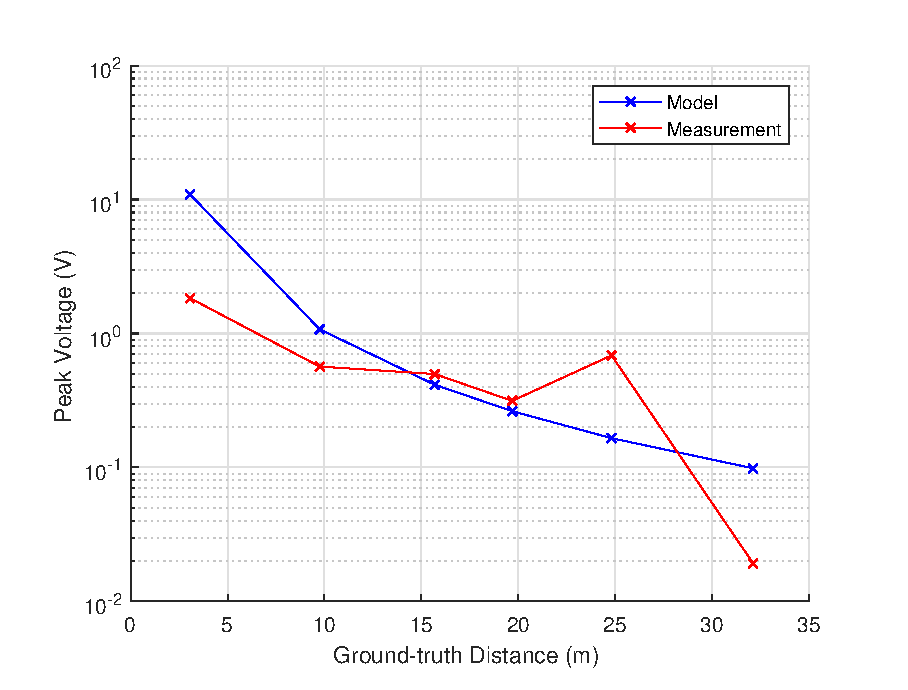
\includegraphics[width=1\textwidth]{figures/chapter_propagation/Res_validation_Vp_distance.eps}
\caption{Peak power of modeled signal and oscilloscope measurements}
\label{fig:prop_valid}
\end{figure}

\chapter{Application of Signal Processing Filters}\label{ch:AFE}
\section{Effect of Filter Characteristics on Signals}
% Therefore, smaller bandpass ripple is suggested to avoid large effect on the signal.
% filter recommendation
In the section, the effects of different filter characteristics on the rise time, time delay, and magnitude attenuation of the signals are studied. The studied filter types include Butterworth filter, Chebyshev filter and Elliptic filters. Since the Bessel filter is a pure analog filter which can not be simulated by MATLAB, its application is not included in this work. The experimented filter characteristics are given in Table~\ref{table:AFE_filterParam}. 
%
\begin{table}[]
\centering
\caption{Filter characteristics}
\label{table:AFE_filterParam}
\begin{tabular}{|l|c|l|l|}
\hline
Type & \multicolumn{1}{l|}{Butterworth} & Chebyshev & Elliptic \\ \hline
Cutoff Frequency & \multicolumn{3}{c|}{2.5 GHz} \\ \hline
Order & \multicolumn{3}{c|}{3, 5, 7} \\ \hline
Passband & - & \multicolumn{2}{c|}{3 dB, 5 dB, 10 dB} \\ \hline
Stopband & \multicolumn{2}{c|}{-} & \multicolumn{1}{c|}{30 dB} \\ \hline
\end{tabular}
\end{table}
%
In the experiment, the pulses reflected from the target were used as the signals feed into the filters. The target was set at 20m ($0.133\mu s$), and white noise arisen from electrical system was generated by the noise model and added to the return pulses. Here, we assume no other distortion or noises acts on the signal. A noise-free signal returned from the same distance was also provided as a reference signal. By comparing with the noise-free signal, the following metrics are used for the evaluation of the influence of the filter on the signals:
\begin{itemize}
  \item Rise-time difference: $\Delta t_r= t_{r, meas} - t_{r, noise-free}$, and $t_{r, noise-free}=3.55ns$;
  \item Time shift: $\Delta t_{peak} = t_{peak, meas} - t_{peak, noise-free}$, and $t_{peak, noise-free}=0.133\mu s$;
  \item Signal magnitude attenuation: $\Delta_P=\frac{P_{means}-P_{noise-free}}{P_{noise-free}}$, and $P_{noise-free} = 20.17\mu W$.
\end{itemize}
The transmit signal and its single-sided power spectrum is given in Figure~\ref{fig:AFE_transmit}, and the return signal contaminated by white noise and its power spectrum is shown in Figure~\ref{fig:AFE_return}. Figure~\ref{fig:AFE_return} shows that the return signal has a noisy spectrum at high frequencies which causes the fluctuation of the signal in time domain. 
\begin{figure}[t!p]
\centering
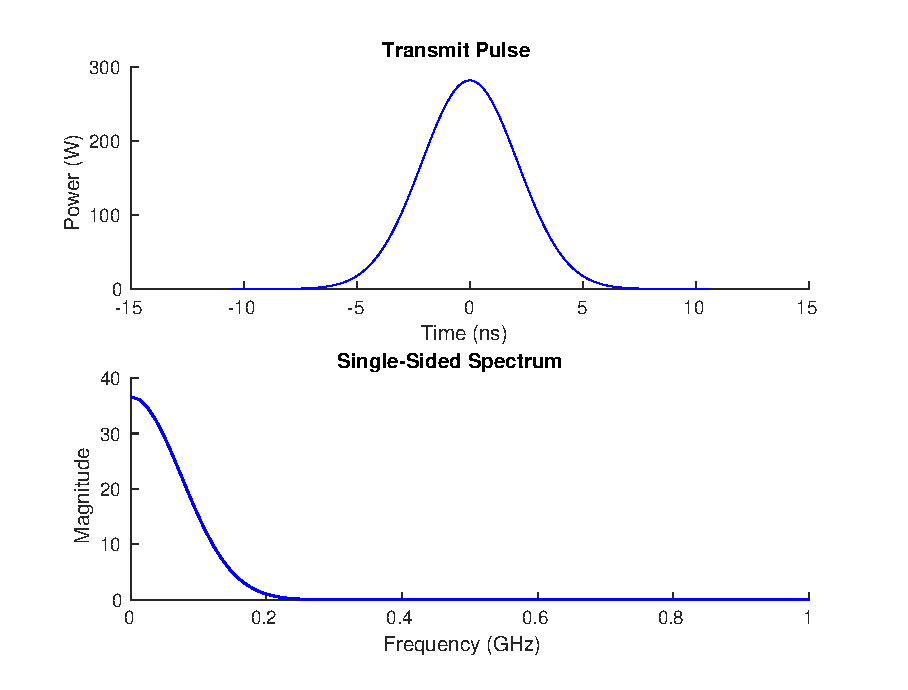
\includegraphics[width=1\textwidth]{figures/chapter_AFE/sig_start.eps}
\caption{Transmit pulse (top) and the single-sided power spectrum (bottom)}
\label{fig:AFE_transmit}
\end{figure}
%
\begin{figure}[t!p]
\centering
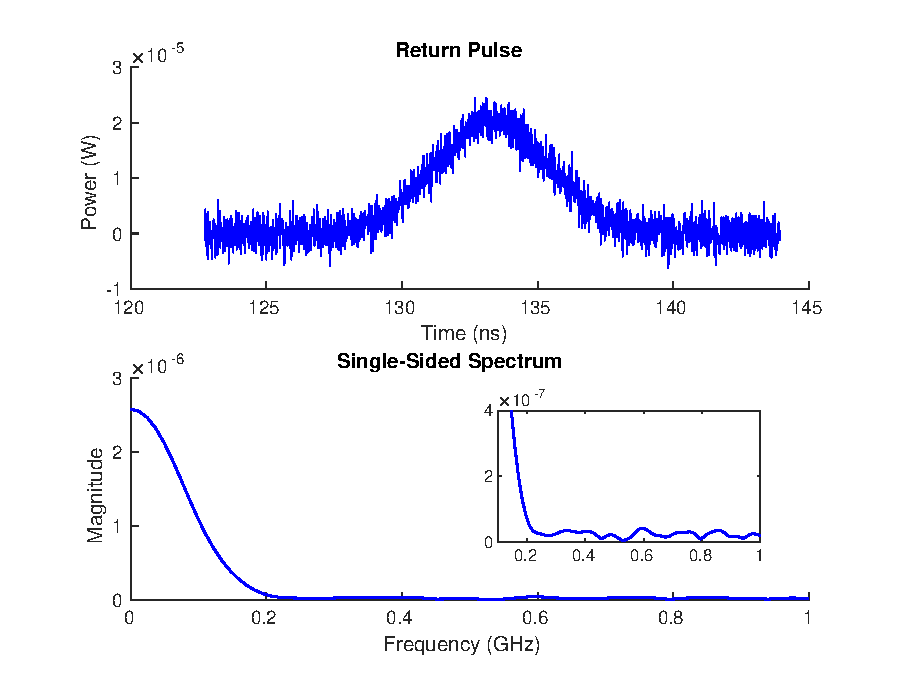
\includegraphics[width=1\textwidth]{figures/chapter_AFE/sig_return.eps}
\caption{Return pulse(top) and the single-sided power spectrum(bottom). The lower portion of the power spectrum is zoomed in and is shown in the sub-figure on the right.}
\label{fig:AFE_return}
\end{figure}
\subsection{Effect of orders}
In the study of the effect of filter order, the passband ripple of the Chebyshev and Elliptic filter was set to 3 dB and the stopband of the Elliptic filter was set to 30 dB. The effects of the order on the signal characteristics are shown in Figure~\ref{fig:AFE_res_orderEffect}. The figure demonstrates that the magnitude attenuation by the filters increases with orders for the Chebyshev and Elliptic filter. The Chebyshev filter has the largest attenuation, followed by the Elliptic filter at the same order, while the effect of the Butterworth filter is very slight. The reason is that the oscillation of the passband ripple of the Chebyshev and Elliptic filter increases with the order, as shown in the magnitude response of the two types of filters (Figure~\ref{fig:AFE_freqResp_chebyr_order}(b) and Figure~\ref{fig:AFE_freqResp_ellip_order}(b)), and the increased ripple at the passband results in larger distortion of the signal magnitude. However, the Butterworth filter has a flat passband (Figure~\ref{fig:AFE_freqResp_butter_order}(b)), so the in-band frequency components are not affected by the change of order.\par
Moreover, the rise time and time shift of the signal also changes with the order. As shown in\todo{change figure, fix ylim} Figure~\ref{fig:AFE_freqResp_butter_order}(c), Figure~\ref{fig:AFE_freqResp_chebyr_order}(c) and Figure~\ref{fig:AFE_freqResp_ellip_order}(c), the nonlinearity of the phase response increases with orders, and the Chebyshev filter has the worst linearity followed by the Elliptic filter. According to Equation~\eqref{eq:backgrnd_AFE_grouddelay}, the non-constant slope of the phase response curve causes group delay distortion of the signal which eventually alters the rise time. Moreover, since the time delay of the signal is equal to the slope of the response curve (group delay), the higher order also results in an increase of the time shift. 
\begin{figure}[h]
\centering
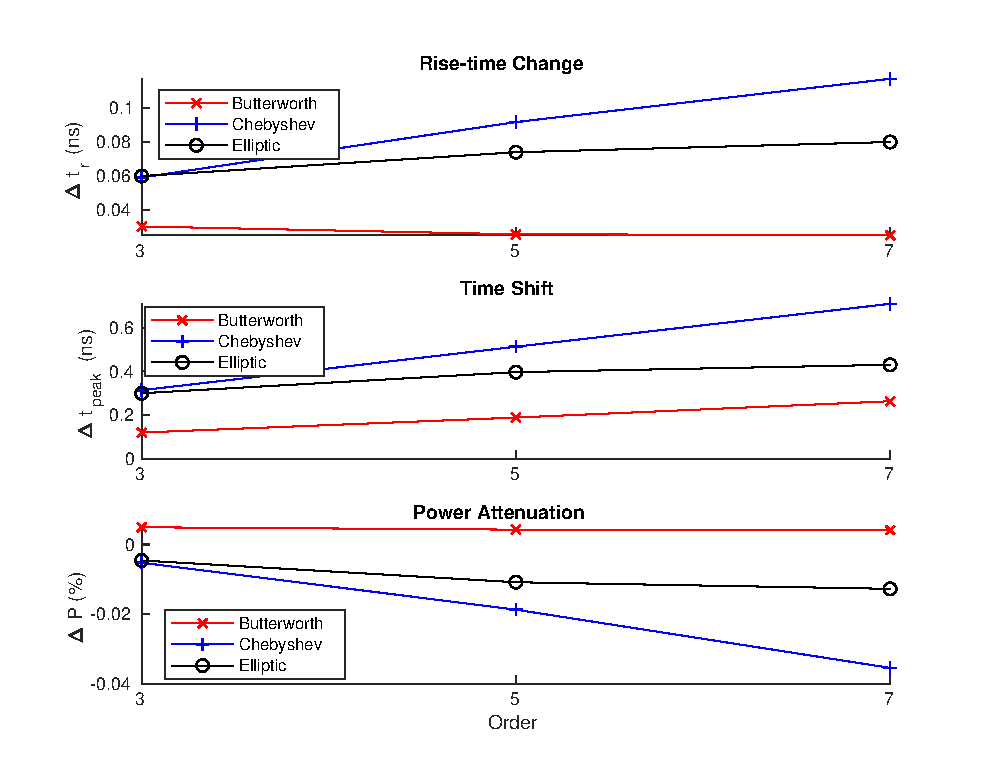
\includegraphics[width=1\textwidth]{figures/chapter_AFE/Effect_order_diff_filter.eps}
\caption{Effect of filters order on the signal characteristics}
\label{fig:AFE_res_orderEffect}
\end{figure}
\begin{figure}[t!p]
\centering
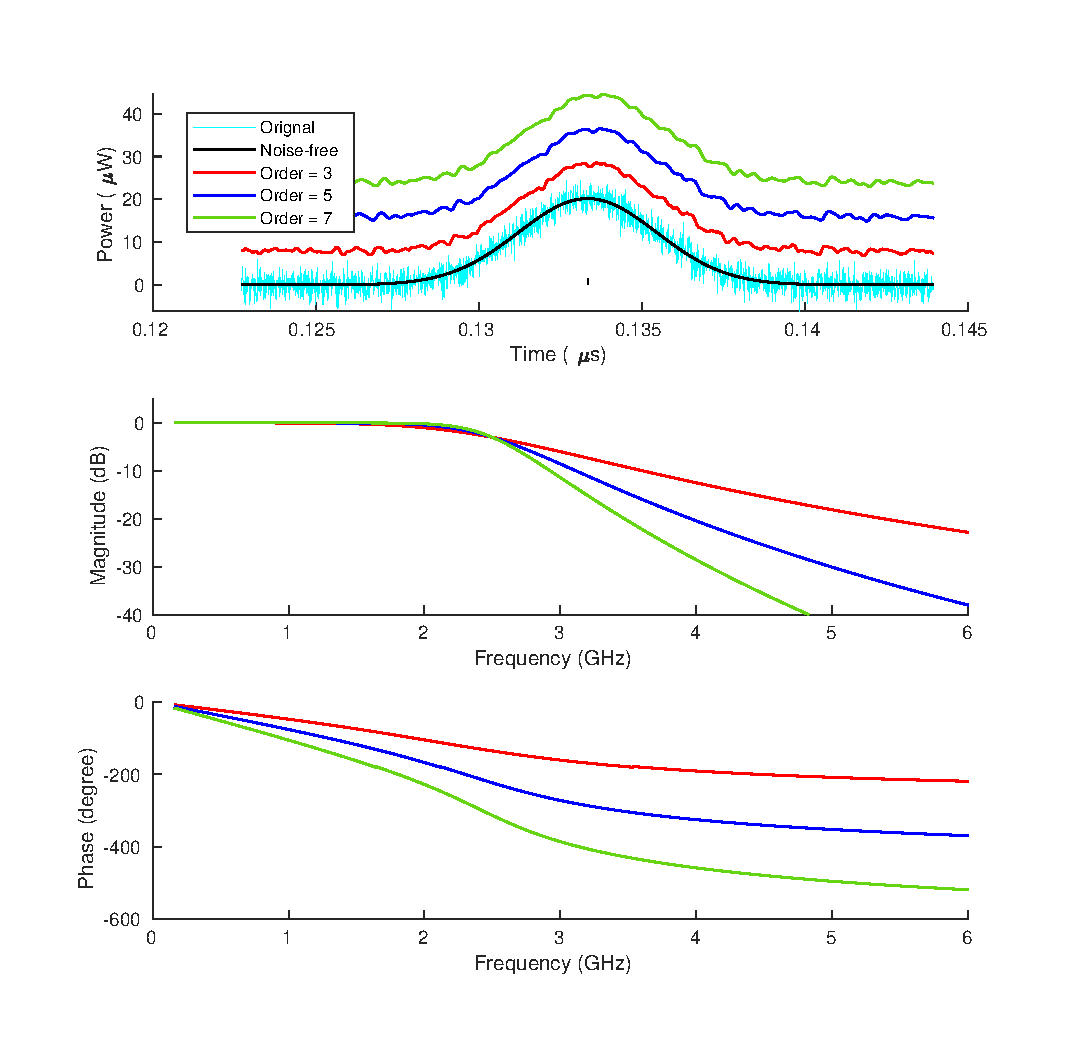
\includegraphics[width=1\textwidth]{figures/chapter_AFE/freq_response_butter_diffOrder.eps}
\caption{Frequency response of Butterworth filter with different orders}
\label{fig:AFE_freqResp_butter_order}
\end{figure}
%
\begin{figure}[t!p]
\centering
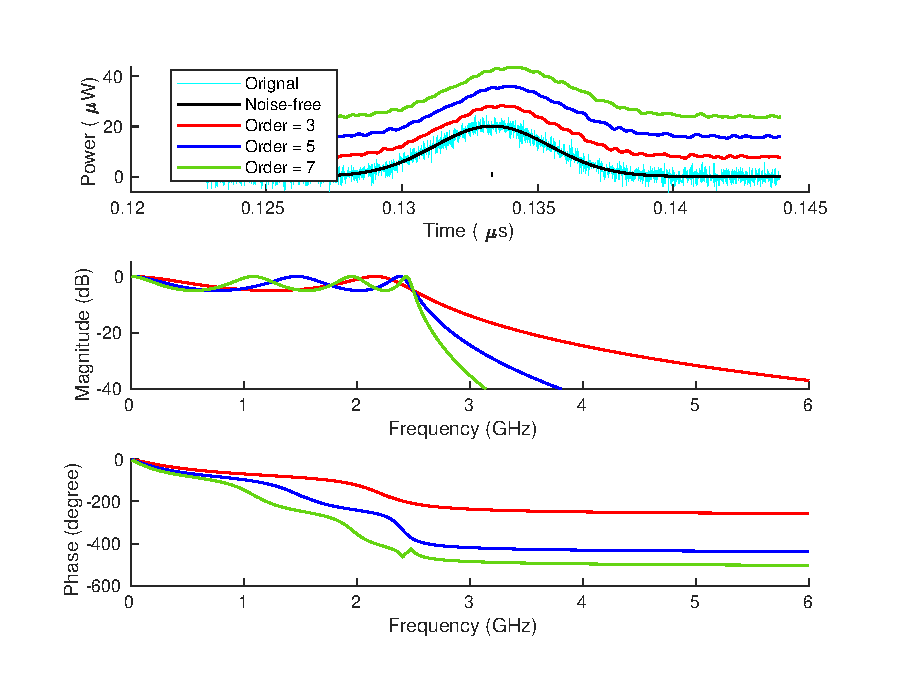
\includegraphics[width=1\textwidth]{figures/chapter_AFE/freq_response_cheby_diffOrder.eps}
\caption{Frequency response of Chebyshev filter with different orders}
\label{fig:AFE_freqResp_chebyr_order}
\end{figure}
\begin{figure}[t!p]
\centering
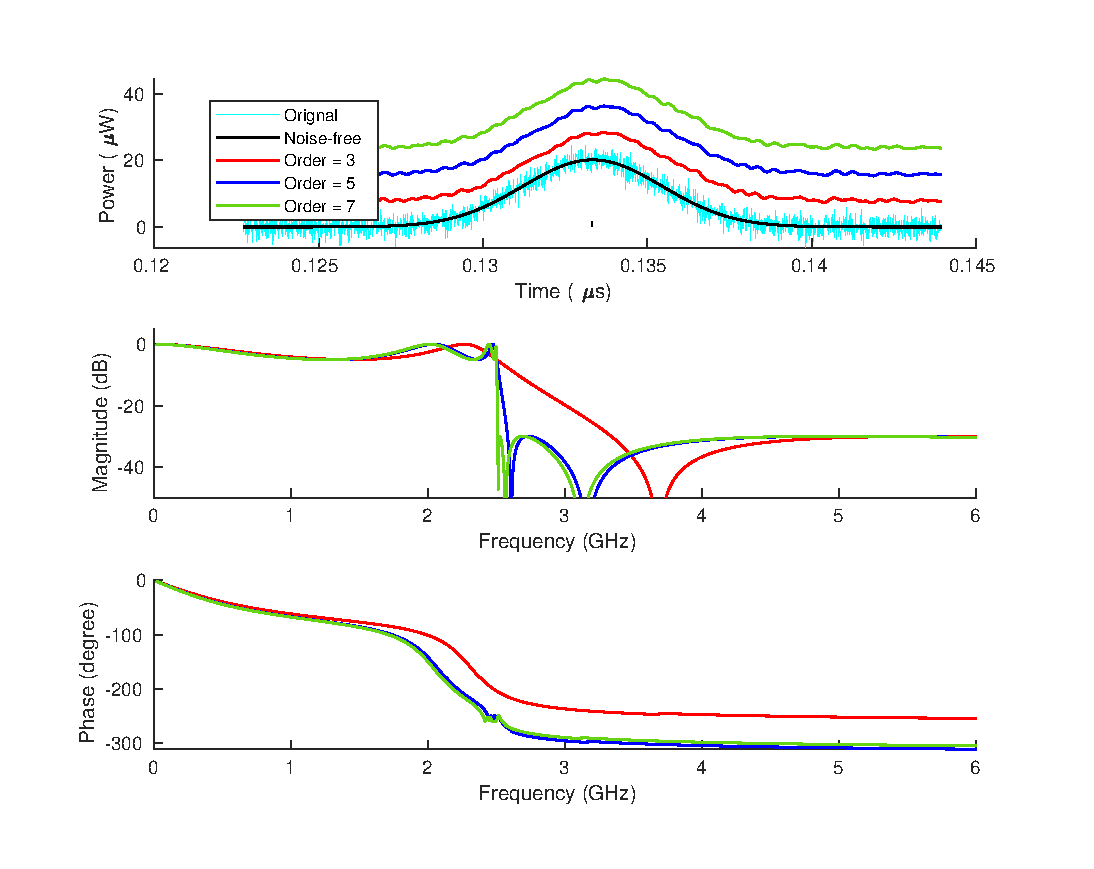
\includegraphics[width=1\textwidth]{figures/chapter_AFE/freq_response_elliptic_diffOrder.eps}
\caption{Frequency response of Elliptic filter with different orders}
\textbf{\label{fig:AFE_freqResp_ellip_order}}
\end{figure}
% Passband
\subsection{Effect of passband ripples}
The effect of passband ripples on the signal characteristics is also studied. In the study, to control the number of variables, the order of all the filters was set to 3 and the stopband ripple of the Elliptic filter remains 30 dB. The signal characteristics after filtering by filters with different passband ripples are presented in Figure~\ref{fig:AFE_res_rppassEffect}, and the results of the Butterworth filter are also provided for comparison. The frequency response of the Chebyshev and Elliptic filter are shown in Figure~\ref{fig:AFE_freqResp_cheby_pass} and Figure~\ref{fig:AFE_freqResp_ellip_pass}.As discussed before, high passband ripple causes a larger magnitude distortion of the signal, resulting in an increase of power attenuation. Furthermore, as the ripple value increases, the phase response becomes more nonlinear, which results in a larger change of rise time and the time shift of the signal. 
%
\begin{figure}[t!p]
\centering
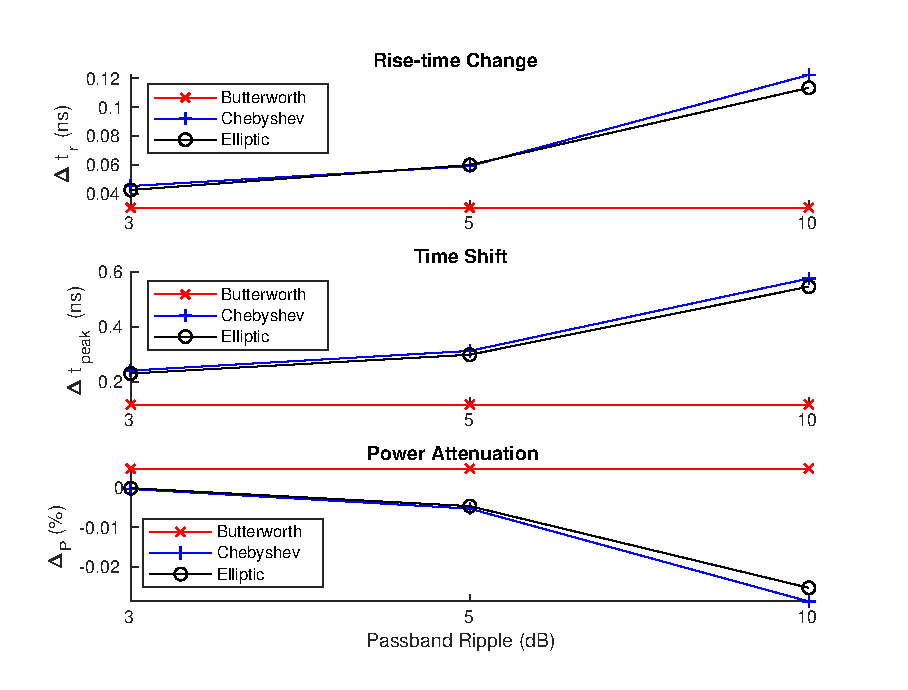
\includegraphics[width=1\textwidth]{figures/chapter_AFE/Effect_rppass_diff_filter.eps}
\caption{Effect of passband ripple order on the signal characteristics}
\label{fig:AFE_res_rppassEffect}
\end{figure}
%
\begin{figure}[t!p]
\centering
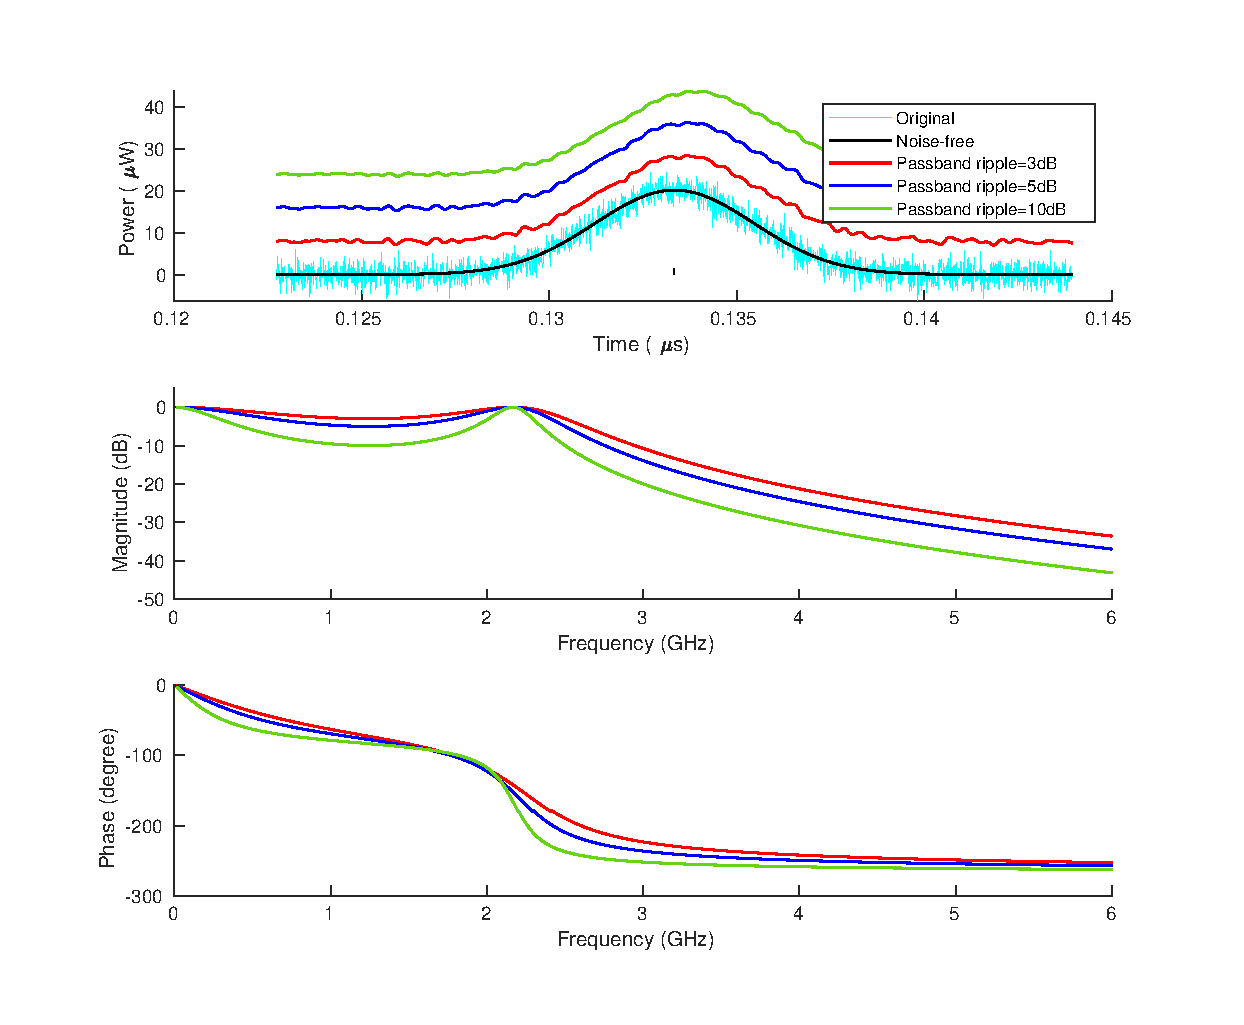
\includegraphics[width=1\textwidth]{figures/chapter_AFE/freq_response_cheby_diffPass.eps}
\caption{Frequency response of Chebyshev filter with different passband ripples}
\label{fig:AFE_freqResp_cheby_pass}
\end{figure}
%
\begin{figure}[t!p]
\centering
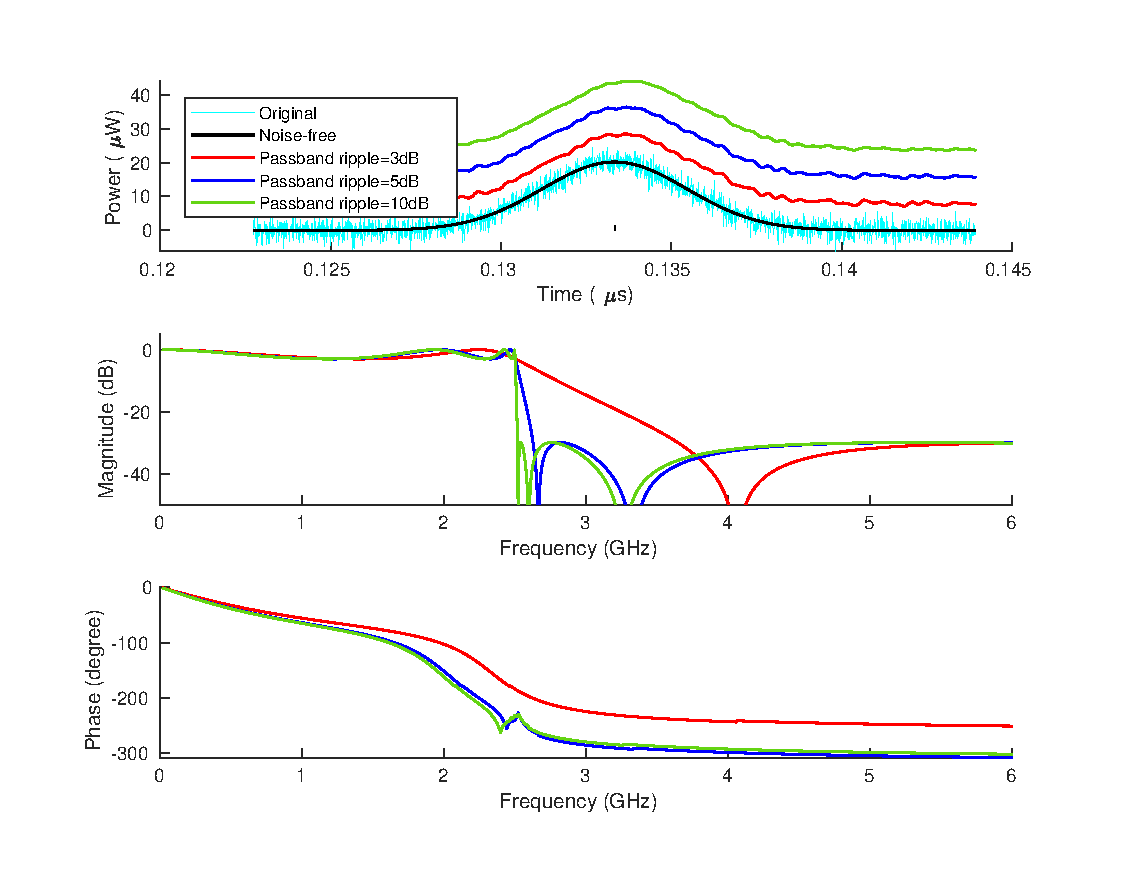
\includegraphics[width=1\textwidth]{figures/chapter_AFE/freq_response_elliptic_diffPass.eps}
\caption{Frequency response of Elliptic filter with different passband ripples}
\textbf{\label{fig:AFE_freqResp_ellip_pass}}
\end{figure}

%% filtfilt
\subsection{Zero-phase filtering}
From the above discussion, we can see the application of filters with nonlinear phase response will cause an increase of rise time and a time delay of the signal. The enlarged rise time and time shift could cause biased distance measurement and increased measurement uncertainty. To reduce the impact on the rise time, one solution is to apply a filter with linear phase response, and the Bessel filter is a desired but the trade-off is that the roll-off of the filter is slower than the Chebyshev and Elliptic filters. To address the time shift, one approach is to apply a filter to both START signal and STOP signal sensed by the receiver. Therefore, the time delay at the two signals are cancelled in the TOF calculation. If in any case no filter is applied to one of the signal, the time delay arisen from the filter can also be calibrated from experiments and be subtracted from the calculated TOF. Additionally, an all-pass filter with a customized phase response according to the time delay can also be added after the original filter to compensate the group delay.\par
In the signal processing, the \emph{zero-phase filtering} can compensate the time shift caused by the filter and provide zero-phase shift. Generally, a signal is only feed into the filter once, which is called ‘forward filtering’. However, the zero-phase filtering has additional step that feeds the signal backwards after the forward filtering. Since backwards filtering causes a negative group delay, the positive and negative group delays are canceled and a zero-phase signal is achieved. The zero-phase filtering can be performed by using any aforementioned type of filters. The effect of the zero-phase filtering on the signal characteristics is also studied in this work. The filtered signals and the resultant characteristics are given in Figure:\ref{fig:AFE_filtfilt} and Table~\ref{table:AFE_res_phaseComp}. In the experiment, the cutoff frequency of the filters was set to 1 GHz, the order of the filters set to 3, the passband ripple 3 dB and stopband ripple 30 dB. From the results we can see the time shift is theoretically eliminated. However, the power attenuation caused the Chebyshev and Elliptic filter is doubled, and rise-time difference also becomes worse. The reason for those effects is that the zero-phase filter actually filters a signal twice, so the distortion of the signal is worsen than the forward filtering. In our case, the signals were actually filtered by filters with a passband ripple of 6 dB. On the other hand, since the Butterworth filter has a flat passband, the distortion caused by Butterworth filter is much less than the other two. Another drawback of the zero-phase filtering is that the entire signal should be available for the zero-phase filtering, which means the zero-phase filtering can not be realized in real-time by an analog circuit but can only be performed offline. Therefore, even though the zero-phase is powerful of removing the time-shift of the signal, it is only limited to offline post-processing signals that are stored beforehand. 
%
\begin{figure}[t!p]
\centering
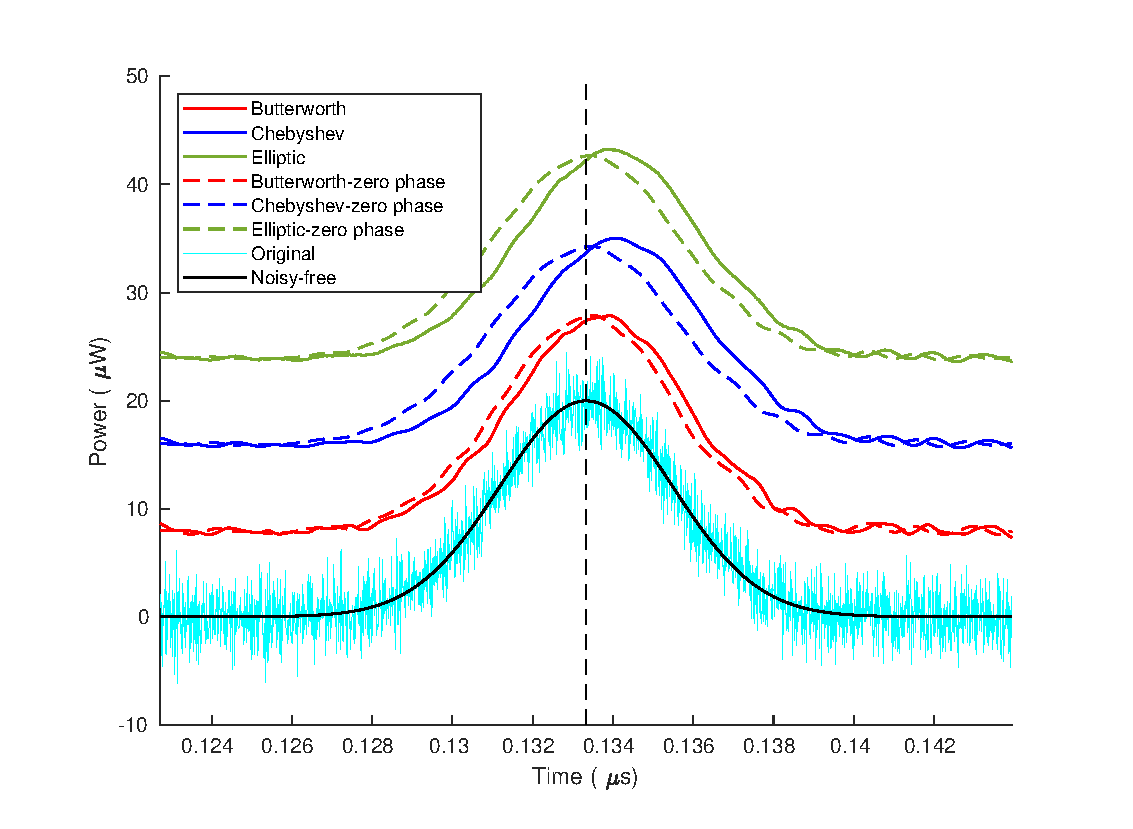
\includegraphics[width=1\textwidth]{figures/chapter_AFE/sig_filtfilt.eps}
\caption{Signal after phase-shift compensation}
\label{fig:AFE_filtfilt}
\end{figure}
%
\begin{table}[h]
\centering
\caption{Result of signal characteristics after phase-shift compensation}
\label{table:AFE_res_phaseComp}
\begin{tabular}{|l|c|c|c|c|c|c|}
\hline
Filter Type & \multicolumn{2}{c|}{Butterworth} & \multicolumn{2}{c|}{Chebyshev} & \multicolumn{2}{c|}{Elliptic} \\ \hline
Phase shift compensation & No & \multicolumn{1}{l|}{zero-phase} & No & \multicolumn{1}{l|}{zero-phase} & No & \multicolumn{1}{l|}{zero-phase} \\ \hline
Rise-time Difference (ns) & 0.042 & 0.037 & 0.061 & 0.218 & 0.061 & 0.196 \\ \hline
Time Shift (ns) & 0.632 & -0.015 & 0.750 & -0.030 & 0.726 & -0.030 \\ \hline
Power Attenuation ratio (\%) & 0.010 & -0.104 & -2.045 & -4.022 & -1.984 & -3.907 \\ \hline
\end{tabular}
\end{table}



%%
% application of filters with different params to sim signals --> Butter is best
% applicadton o filters to real signal, compare w/o filt and w/ filt. -> ADC MF


%%\subsection{Digital Filters}

%% filter implementation: LP filter can attenuate the signal amplitude if fcut is inside the BW: [Figure 4, Challenges in miniaturized automotive long-range lidar system design]

\chapter{Time Discrimination-TDC}\label{ch:TDC}
% walk error - amplitude, compare with analytical results
% compare look up table between real and simulate relation
% results w/o fitlers and results after filter
% error for different methods
In this section, the TDC modeling will be introduced first followed by the application of different timing algorithms to simulated return signals from different target distances. The slew-rate compensation is not included due to the usage of two thresholds. The two-threshold configuration makes weak return signal invisible to the system because when the amplitude of the return pulse is lower than the higher threshold, the comparator will not be triggered, and the algorithm will ignore the pulse. In addition, the time-variant thresholding is not included in this section either since the R and C values of the photon detector are not available in this study, which makes it difficult to calibrate the parameter A and B in Equation \eqref{eq:TDC_time1}, and therefore, modeling the time-variant thresholding is impractical.
% TDC modeling
\section{TDC Modeling}
%{Propagation delay}
\subsection{Propagation delay}
As shown in Figure \ref{fig:TDC_schematic}, the comparator is one of the key components of the TDC. In practice, a TDC circuit requires a small amount of time to respond and propagate signals for voltage comparison, so the comparators have a propagation delay, which limits the fastest frequency of a signal the TDC can process [4]. However, on the other hand, even though the propagation delay restrains the frequency of the signal to be processed, slower fluctuation still exists in the transient signal inside the comparator, caused by the unstable transient response of the electrical device to high-frequency oscillation. To model the response of the TDC to the input analog signal, we have to simulate the transient signal, but the transient response of an electrical device to a rapid oscillating signal is usually ill-defined, which makes the modeling difficult. In this study, inspired by Wahab [1], we approximated the transient signal by sub-sampling the original ‘continuous' signal with a sampling rate of 2GHz and smoothing the sub-sampled signal by a spline-line fitting, assuming no additional high-frequency noises were added to the transient signals before comparison. One should note that the approximation is one of the simplified versions of the transient signal. In a real device, the transient signal may not follow the same behavior as described above. Moreover, the sub-sampling rate (2 GHz) was obtained from the bandwidth of a high-speed comparator defined by its propagation delay $\tau_{delay}$ (0.25 ns): $bandwidth = 1/2\tau_{delay}$ [2]. An example of the signal after subsampling is shown in Figure \ref{fig:TDC_subsampling}.
% If a signal was sampled at a frequency lower than 2 GHz, no sub-sampling was performed before the spline-line fitting because the bandwidth of the signal is already smaller than the bandwidth of the comparator.
\begin{figure}[t!p]
\centering
\includegraphics[width=.8\textwidth]{figures/chapter7_TDC/fig_subsampling.jpg}
\caption{The ‘continuous’ return signal after subsampling}
\label{fig:TDC_subsampling}
\end{figure}
% Linear Interpolation
\subsection{Linear interpolation}
The sampling rate of the signal is set to 100GHz or 10ps, and the TDC resolution was set to 1 ps [3]. The resolution was achieved in the TDC model by linearly interpolating the transient signals to a grid of 1 ps, and whenever a point on the grid excessed the threshold, the corresponding time was measured as the arrival time. The linear interpolation is applied to the trigger events of all the TDC-based timing algorithms. An example of the interpolation for the traditional leading-edge algorithm is shown in Figure \ref{fig:TDCinterpolation}.
\begin{figure}[t!p]
\centering
\includegraphics[width=.8\textwidth]{figures/chapter7_TDC/TDC_interpolation.jpg}
\caption{Illustration of interpolation for leading-edge detection }
\label{fig:TDCinterpolation}
\end{figure}
% threshold
\subsection{TDC trigger threshold}
The setting of the trigger threshold of a TDC is also important because too low or too high threshold will increase the false triggering by the noise (PFA) or decrease the sensitivity of the algorithm to weak return signals (PD). To balance the trade-off between PFA and PD, in this study we determine the threshold by the probability of false positive. Here we assume the noise of the electrical system is Gaussian distributed white noise. Theoretically, the threshold can be determined by:
\begin{align} \label{eq:TDC_threshold}
    V_{th}=\sigma_0Q^{-1}\left(P_{fa}\right)+\mu_0
\end{align}
where $\mu_0$ is the mean of the noise which is equal to zero, $\sigma_0$ is the STD of the noise of the signal with laser off, and Q is the complementary cumulative distribution function (CCDF) of the Gaussian white noise, defined by
\begin{align}
    Q\left(x\right)=\frac{1}{2}efc\left(\frac{x}{\sqrt2}\right)
\end{align}
% experiement
\section{Experiment and Timing algorithms}
\subsection{Experimental design}
Monte-Carlo experiment was conducted using 500 observations of transmit and return signals. The target distance ranges from 5 to 60m with an increment of 2.5m. The return signals were generated by the pulse model, the propagation model, and the noise model. The key parameters used in those models are given below with other parameters unchanged.
\begin{table}
\caption{{Parameters in lidar models}}
\centering
\label{table:lidarspec}
\begin{tabular}{|l|l|l|}
\hline
Parameters    & Values \\ \hline
Peak power & $300 W$              \\ \hline
Sampling rate & $100~GHz$      \\ \hline
Target reflectivity & $10\%$     \\ \hline
BW due to comparator propagation delay & $2~GHz$        \\ \hline
\end{tabular}%
\end{table}
% threshold
\subsection{TDC trigger threshold}
The PFA is preset to 0.001 in this study, and it was evaluated on 100 observations of noise signals with the laser off. The noise signals were generated by the noise model, each of which has 2123 data points, that is, there are total 212300 points in the 100 observations. The measured PFA is calculated by:
\begin{align}
    P_{fa,meas}=\frac{\sum_{m} k_m}{MN}
\end{align}
where $k_m$ is the number of data points in the m-th observation that are larger than the TDC threshold, and M and N are the number of observation and the number of points in each observation, respectively. The measured $P_{FA} = 9.8917e-4$, which is close to predefined $P_{FA}$.
% time algorithm
\subsection{Timing Algorithm}
The traditional leading-edge timing algorithm, the leading-edge algorithm with TOT compensation and the CFD algorithm were applied to both transmit and return signals, and the TOF is estimated by the difference between the arrival time of the return and transmit signal. The constant fraction of the CFD is set to $30\%$ of the peak power, and the arming threshold is set the same as the TDC threshold. The Mean error and RMS error of the distance measurement are used for the evaluation of the performance of the timing algorithms.
% result and discussion
\section{Results and Discussion}
\subsection{Original results}
The results of the different timing algorithms are given in Figure \ref{fig:TDC_Error_beforeFilter}. From the mean error, we can see that the leading-edge algorithm has an obvious positive bias from the ground truth, and it increases with distance. The positive bias is caused by the walk error. As the distance increases, the amplitude difference between the transmit and return signals increases, which results in a larger walk error. Compared to the traditional leading-edge algorithm, the bias from the results of the TOT compensation and the CFD algorithm is much less. The results of those two algorithms are given in Figure \ref{fig:TDC_Error_beforeFilter}(b) to illustrate the details. 
\begin{figure}[t!p]
\centering
\includegraphics[width=.8\textwidth]{figures/chapter7_TDC/fig_distError_snr.jpg}
\caption{Mean error and RMS error of different timing algorithms}
\label{fig:TDC_Error_beforeFilter}
\end{figure}
The CFD has almost bias at all the distances, while the TOT compensation has increasing negative mean error as distance increases. There are two factors that contribute to the mean error. Note that the TOT compensation calculates the TOF by
\begin{align} \label{eq:TDC_TOT}
TOF=t_{lead}-\Delta_w-t_{start}    
\end{align}
where $t_{lead}$ is the timestamp of the trigger event at the leading edge of a signal, $\Delta_w$ is the walk error obtained from TOT curve, and $t_{start}$ is the arrival time of the transmit signal. The major factor of the negative bias is the inaccurate measurement of $t_{lead}$. As known, the noise on the leading edge of the signal becomes comparative to the pulse at further distance, which causes early triggering of the TDC. An example is given in Figure \ref{fig:TDC_earlyTrigger}, in which the TDC is triggered earlier than it is supposed to be. In that case the $t_{lead}$ is smaller than the ground-truth $t_{lead}$, resulting in a smaller TOF estimation according to Equation \eqref{eq:TDC_TOT}. The statistic measurement of the 500 observations at distance 15m also provides evidence that the measured $t_{lead}$ is 0.15ns (or distance offset of 0.0233m) less than the ground-truth value measured from the noise-free signals. Another factor for the mean error is the inaccurate measurement of the TOT when the SNR is low. Taking the 15m distance for example, the measured TOT from noisy return signals in the experiment is larger than the TOT of the corresponding noise-free signals, which results in that the derived walk error is 0.002m smaller than the ground-truth walk error. However, the inaccurate TOT measurement only contributes slightly to the mean error compared to the early triggering.
\begin{figure}[t!p]
\centering
\includegraphics[width=.8\textwidth]{figures/chapter7_TDC/signal_TOT_d_15_trigger.jpg}
\caption{Illustration of early triggering caused by the noise on the leading edge}
\label{fig:TDC_earlyTrigger}
\end{figure}
From the RMS error, we can see all the algorithms are subject to the noise on the signal when the SNR decreases. The traditional leading-edge algorithm is very sensitive to the noise on the signal, while the effect of the noise is compensated to some extent in the TOT algorithm because both the leading edge and falling edge of the signal are taken into account. The CFD algorithm has the least RMS error because the random noise is canceled when the negative attenuated signal is added to the delay signal. However, the CFD method does not work for low SNR conditions (<21.47 dB), because in those cases the amplitude of the attenuated signal is lower than the arming threshold, and the signal is ignored by the algorithm.
\subsection{Low-pass filter}
To reduce the effect of the noise on the TOF estimation, an LP filter with fcut= 0.4GHz was applied to the return signals before the timing algorithms, and the phase shift is compensated. One should note that small orders of the LP should be selected to avoid distortion of the pulse shape. Otherwise, the results of the TOT compensation and the CFD will be affected. The detailed information is given in Section. An example of the filtered signal at a distance of 15 m is given in Figure \ref{fig:TDC_sig_filt}.
\begin{figure}[t!p]
\centering
\includegraphics[width=.8\textwidth]{figures/chapter7_TDC/signal_filtered_d15.jpg}
\caption{Original and the filtered signal at a distance of 15m}
\label{fig:TDC_sig_filt}
\end{figure}
\subsection{Results after filtering}
The results after LP filtering are shown in Figure \ref{fig:TDC_Error_afterFilter}. From the Mean error, we can see the positive bias still exists in the traditional leading-edge algorithm because the bias is caused by the walk error which cannot be resolved by the LP filter. On the contrary, the LP filter improves the mean error of the CFD and the TOT compensation. An example of the filtered signal is given in Figure \ref{fig:TDC_earlyTrigger_filt}, in which the noise on the leading edge of the signal is significantly reduced. Statistical results at distance 15m also show the $t_{lead}$ of the filtered noisy signal is only 0.04ns (0.006m distance offset) smaller than the one of noise-free signals, and the difference of walk error is changed to 0.0038m converted to distance. The reduction of the $t_{lead}$ difference also demonstrates the influence of the noise on the TOF measurements. On the other hand, the RMS error of all the algorithms are reduced after the filtering, and the CFD still has the least RMS error followed by the TOT compensation.
\begin{figure}[t!p]
\centering
\includegraphics[width=.8\textwidth]{figures/chapter7_TDC/fig_distError_snr_filter.jpg}
\caption{Mean error and RMS error after filtering}
\label{fig:TDC_Error_afterFilter}
\end{figure}

\begin{figure}[t!p]
\centering
\includegraphics[width=.8\textwidth]{figures/chapter7_TDC/signal_TOT_d_15_trigger_filt.jpg}
\caption{Signal after filtering. Compared to Figure14, the early triggering on the leading edge is significantly reduced by the LP filter}
\label{fig:TDC_earlyTrigger_filt}
\end{figure}
%%%%!!!!!!!!!!!!!!!!!!!!! todo
% check value of distance and corresponding SNR
% In the future, ene could set a dynamic criteria of pulse width  with distance, according to the trigger model and pulse width in use..

% trigger mode discussion
%%%%%%%%%%%%%%%%%%%%%%%%%%%%%%%%%%%%%%%%%%%%%

\chapter{Time Discrimination-ADC}\label{ch:ADC_BM}
\section{Problem Description}
In addition to the TDC-based approaches, we can also use ADC. The ADC-based time discrimination is using ADC to convert analog signals output from a detector to digital signals, and measure the time of the digital returning pulse. The structure of the ADC-based discriminator is shown in Figure~\ref{fig:schematic_ADC}. The time discrimination can be achieved by applying digital versions of the TDC-based timing algorithms to the digital signals, or by taking advantages of the shape information contained in the digital signals.
\subsection{Digital version of the analog timing techniques}
 The digital versions of the TDC-based timing algorithms include the aforementioned algorithms like leading-edge detection techniques and CFDs. The details of those methods are described in the above sections and are skipped here, but one should notice some drawbacks of the digital version algorithms. One is that for the digital signals, the threshold generally does not coincide to the sample points of the signal. Therefore, interpolation between neighborhood samples is needed to find the exact time mark corresponding to the threshold value. Linear interpolation is a common selection, but the interpolation could affect the timing accuracy, depending on the local linearity of the signal. More specifically, if the curvature of a signal in the proximity of the threshold is large (the pulse has a nonlinear shape), time walk could occur. Note that this walk error is different than the walk error mentioned in the TDC-based approaches. The effect of the curvature is illustrated in Fig \todo{(Fig10.27 Mahammad book). }
\subsection{Detector and Estimator}
% The digital version of the TDC-based techniques utilizes the ADC as a TDC, which limits the potential of the ADC since the valuable shape information contained in the digital signal is not taken into consideration which could improve the accuracy of signal detection and estimation. Therefore, we proposed the time discrimination algorithms that take advantage the shape information and are generally composed of a detector and an estimator. The detector is to take the digital signal output from an ADC and determine the presence or absence of a predefined signal from a signal contaminated by noise. In our case, that is if a Gaussian pulse with certain characteristics (\ie rise time, pulse width, \etc) is present in the returning signal. The absence or presence of a return pulse is denoted by a binary hypothesis test $\mathcal{H}_1$: pulse or $\mathcal{H}_0$: noise.Subsequently, if the pulse is present, an estimator is needed to estimate the values of the parameters of the signal (the arrival time of return pulses in our case). \\
% In this section, we first introduce the fundamentals of the ADC, followed by two algorithms that determines the presence of a return signal and estimates the arrival time of the return pulse.




%%


%% + literature review of detectors and estimators: peak, LSE, MF ...
% \subsubsection{Estimator}
% Many different estimators are available for extraction of signal parameters, \eg the arrival time of a signal, ranging from the simple peak estimator(PE) and time-over-threshold estimator by averaging the detection of the leading and falling edge of a signal, to more advanced Maximum Likelihood Estimator(MLE) and Least Square Estimator(LSE). This work will focus on the PE, MLE, and LSE.The theory will be introduced, followed by the implementation of the estimators to synthetic and real signals.

% \subsubsection{Peak Estimator}
% The PE is straightforward and efficient and has been widely applied to time-of-flight determination and object recognition using lidar and ultrasonic sensors measurements\cite{Steinvall2000EffectsSections,Steinvall2001Three-dimensionalModeling,Steinvall2007,Steinvall2005RangeRadars,Der1997SimulationMeasurements,Gronwall2006GroundApplications,richmond2010direct,Anitha2011Time-of-FlightTechniques}.The peak estimator is either used directly on the raw analog signal or followed by a matched filter and estimate the peak of the convolution result\cite{Der1997SimulationMeasurements}.


 
% \subsection{Maximum Likelihood Estimator} \label{sec:MLE}
% MLE is widely used, 
% papers: steinvall2005range (fit to gaussian), Buschelman, Joly, petrick, tomi



The digital version of the analog timing techniques that utilize the ADC as a TDC limits the potential of the ADC because the shape information of the digital signal which is valuable to improve the accuracy of signal detection and estimation is ignored. In this section, the time discrimination algorithms that capture the characteristics of the pulse are introduced, which is called ADC-based algorithms. The ADC-based timing algorithms are generally composed of a detector and an estimator. The function of the detector is to take the signal collected by an ADC and determine the presence or absence of a predefined signal from the raw signal contaminated by noise. If a pulse is detected, an estimator is needed to estimate the values of the parameters of the signal by mathematically modeling the signal. In our case, the detector is to determine if a return pulse with certain characteristics (\ie shape, rise time, and pulse width, \etc) exists in the collected signal, and estimate the arrival time of the pulse if it is present. In this section, we will focus on two detection and estimation algorithms: centroid-based detection and estimation algorithm(centroid-method) and Neyman-Pearson(NP) detector (or Matched filter). The principle of the algorithms will be illustrated first followed by the application of the algorithms to simulated signals and/or signals collected from real experiments. The centroid detector will be introduced in this section and the Matched filter will be introduced in Chapter~\ref{ch:NP}.

\subsection{Data pre-processing}
To reduce the deterioration of the outliers on the detection algorithms, the digital signals are filtered by a median filter with a kernel with a size of 3 or 5. Small size of kernels were used to avoid distortion of the signal due to the filter. Examples of the signals before and after filtering are shown in \todo{Figure}. The median filter efficiently removes the sparse random outliers, but not the effect is not obvious on frequently occurring noises. %add median filter%

% %
%  Bench-mark detection
% %
\section{Benchmark Detection and Estimation}
\subsection{Metrics for signal detection}\label{sec:bm_metrics}
In the benchmark detection, two metrics are utilized for the hypothesis determination of a return signal. The metrics include the number of points of a signal above the ADC threshold and the pulse width of the signal. In this section, the metrics and the corresponding criterion are defined first, followed by an introduction of the algorithm used for the pulse width calculation.
\subsubsection{Metric 1: Number of points above threshold}
Strong random noises could false-trigger an ADC, but it is very unlikely a large number of consecutive data points of the random noise could excess the threshold. In this case, we use the number of data points of a signal above the ADC threshold (\abbr number above threshold or NaT) as the first metric to distinguish the false-triggering induced by random noise. Usually, the ADC threshold is set at a constant value (\ie 3x noise floor), so when the amplitude of a signal changes, the NaT varies in a range according to the target distance, and stronger signals have a larger value of NaT. To make the metric applicable to signals from different distances, a range of the NaT is defined, and the upper and lower bound of the range is determined by measuring the NaT of noise-free return signals from the shortest and furthest distance studied in this work, specifically, $2~m$ and $300~m$. The corresponding SNRs are $60~dB$ and $8~dB$ and the measured NaTs are 52 points and 10 points, respectively. Therefore, when the ADC receives a signal the NaT of a return signal is counted first, and if the NaT exceeds the range of 10 and 52, the signal is considered to be $\hzero$.
% Metric 2: pulse width
\subsubsection{Metric 2: Pulse width}
Usually, the pulse width of a signal remains constant through the whole signal propagation, assuming negligible distortion of the pulse shape due to the reflection by molecules in the atmosphere and the response time of electrical systems. In this case, we can determine the hypothesis of a return signal by comparing its pulse width with the one of the transmit pulse. The expression of the pulse width of a signal can be derived from Equation \eqref{eq:pw}, such that
\begin{equation} \label{eq:bm_pw}
    \Delta t_w = \frac{E}{P_{r, peak}},
\end{equation}
assuming the approximation for the pulse energy mentioned in Section~\ref{sec:pw} also holds for digital signals. Theoretically, the energy of a signal can be obtained by integrating the signal over an infinitely long time duration, while in practice the signal is truncated due to a finite number of points that can be collected by an ADC. Similar to Metric 1, to determine the criteria, the pulse width of noise-free signals from the shortest and furthest distance was calculated using the method that will be introduced in Section~\ref{sec:bm_pw_cal}. The measured pulse width ranges from $4.91~ns$ (SNR is $8~dB$) to $5.42~ns$ (SNR is $60~dB$), and the variation of the pulse width from the mean value is $0.51~ns$ or $10\%$ of the mean. Therefore, a tolerance of the measured pulse width is defined, such that if the difference between the measured pulse width $\Delta t_{w,meas}$ and the reference pulse width $\Delta t_{w,ref}$ is smaller than $10\%$ of the reference, the signal passes Metric 2. In this study, the reference pulse width is $5.17~ns$. Mathematically, we claim the signal passes Metric 2 if
\begin{equation}\label{eq:bm_cri2}
    |\Delta t_{w, meas} - \Delta t_{w,ref}| < 10\%\Delta t_{w,ref}
\end{equation}\par
\subsubsection{Signal detection}
After defining the metric and the corresponding criterion, we can follow the flowchart shown in Figure~\ref{fig:bm_flowchart} to determine the hypothesis of a return signal. In the detection process, the counting of NaT is straightforward, but the pulse width needs to be calculated from the signal which will be illustrated next.
\begin{figure}[htb] % position options
\centering
\graphicspath{ {figures/} }
\includegraphics[width=0.5\textwidth]{figures/chapter6_ADC/BM_flowchart.png}
\caption{Flow chart of benchmark detection algorithm}
\label{fig:bm_flowchart}
\end{figure}
% pulse width calculation
\subsection{Pulse width calculation} \label{sec:bm_pw_cal}
According to Equation \eqref{eq:bm_pw}, we need to obtain the energy and the peak power of a signal before calculating the pulse width. We first define a polygon with vertices as the data points of a signal. An example of the polygon is shown in Figure~\ref{fig:bm_polygon}. 
\begin{figure}[htb] % position options
\centering
\graphicspath{ {figures/} }
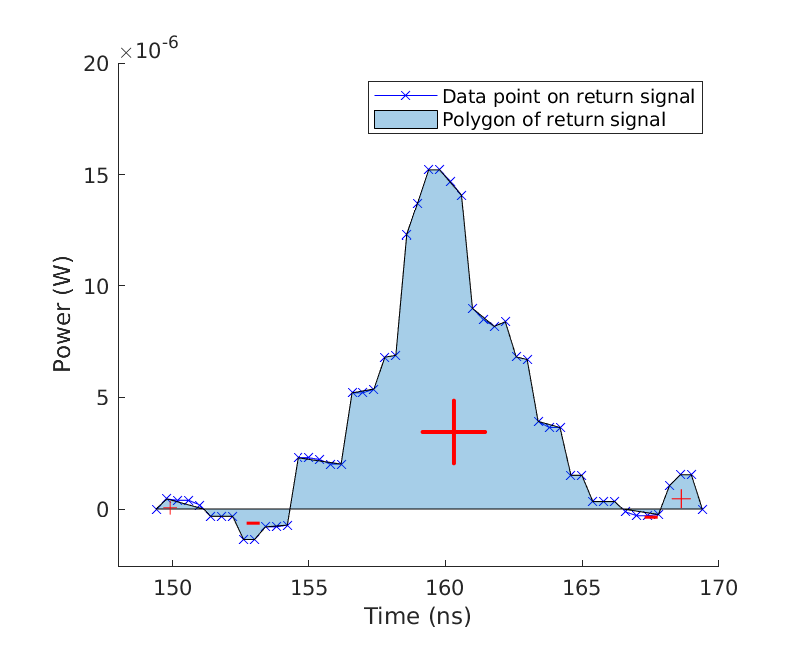
\includegraphics[width=0.8\textwidth]{figures/chapter6_ADC/polygon.eps}
\caption{Example of a polygon defined by data points of a return signal. Regions with '$+$' signs have positive area and regions with '$-$' sign have negative area.}
\label{fig:bm_polygon}
\end{figure}
The energy of the signal was approximated to be equal to the area of the polygon, which can be obtained numerically, by dividing the polygon into several triangles or rectangles and adding the area of each region together\citep{bourke1988calculating}. The mathematical expression is
\begin{equation}\label{eq:area} %% this equation is equivalent to the rieman sum
    A=\frac{1}{2}\sum\limits_{n=1}^{N}(t_nP_{r,n+1}-t_{n+1}P_{r,n}).
\end{equation}
where the $n$-th vertex of the polygon is denoted by $(t_n, P_{r,n})$ and $t_n$ and $P_{r,n}$ are the timestamp and the power value of the point, respectively. $N$ is the total number of data points in a signal. Since the power offset of the digital signal is removed by the ADC in advance, the power allows having negative values, which results in a self-crossing polygon, meaning the sides of the polygon intersect with itself. The negative values and the resultant negative areas of the self-intersecting polygon result in cancellation between the positive and negatives areas. The cancellation is consistent with our expectation that the energy of a signal having power with the same amplitudes but opposite signs is zero.\par
The peak power can be approximated by the \textit{y}-centroid $C_y$ of the polygon using
\begin{equation}\label{eq:bm_peakpower}
    P_{r,peak}=F_c\cdot C_y
\end{equation}
where $F_c$ is a constant factor and $F_c\approx3$. The value of $3$ is derived from combining Equation \eqref{eq:pulsemodel} and the fact that the height of a Gaussian pulse $h_{pulse}\approx2.828C_y$. The factor $F_c$ indicates that the peak power of a Gaussian pulse is always $F_c$ times the \textit{y}-centroid regardless of the signal amplitude. The constant relationship provides a more stable way of estimating the peak power than directly measuring the peak value of a pulse which is subject to large fluctuation due to the noise at the peak.\par
Applying the same approach in Equation \eqref{eq:area}, the centroid of the polygon can be obtained using the area $A$ by \citep{bourke1988calculating}:
\begin{align}
\label{eq:cen_x}
C_x=&\frac{1}{6A}\sum\limits_{n=1}^{N}(t_n+t_{n+1})(t_nP_{r,n+1}-x_{n+1}P_{r,n})\\
\label{eq:cen_y}
C_y=&\frac{1}{6A}\sum\limits_{n=1}^{N}(P_{r,n}+P_{r,n+1})(t_nP_{r,n+1}-x_{n+1}P_{r,n})
\end{align}
One should note that using Equation \eqref{eq:cen_x} and \eqref{eq:cen_y} on self-intersecting polygons will result in unexpected results \citep{bourke1988calculating}. Therefore, instead of using all the data points of a signal, only the points above zero are used for the centroid calculation. Also, to close a polygon the value of $P_{r, N+1}$ at $n=N$ is set equal to the value of $P_{r,1}$ in Equation \eqref{eq:area}, \eqref{eq:cen_x} and \eqref{eq:cen_y}, and to ensure the area cancellation, the value of $P_{r,N}$ and $P_{r,1}$ is set to zero, \ie $P_{r,1}=P_{r,N}=0$.\par
Now, given the energy $E$ and the centroid of the polygon $(C_x, C_y)$, the pulse width of a signal can be obtained by
\begin{equation}
    \Delta t_w = \frac{E}{F_c\cdot C_y}.
\end{equation}
%Estimation of arrival tim%
\subsection{Estimation of arrival time}
After the determination of the hypothesis of a signal, the arrival time of return pulses should be estimated. A simple way for the estimation is to use the timestamp of the peak of a pulse. However, the noise on the peak of a signal could impact the measurement accuracy and the result is also limited by the ADC resolution. Alternatively, we can approximate the lateral position of the peak by the \textit{x}-centroid of the signal, and use the timestamp of $C_x$ as the arrival time:
\begin{equation} \label{eq:bm_arrivalTime}
    t_{STOP}=C_x
\end{equation}
In this case, the resultant TOF and distance measurement is much less sensitive to the noise on the signal, and arrival time smaller than the ADC resolution can be resolved. To further improve the measurement accuracy, one can also use the data above the ADC threshold instead of the data above zero for Equation \eqref{eq:bm_arrivalTime}. It is because the data points above the threshold contain less noise than the data covering the whole noisy leading and falling edge. For a detailed discussion of using different data sets, please refer Section \ref{sec:bm_result}. One should note that the data above the threshold should not be used to calculate the \textit{y}-centroid of a signal, since the constant factor $F_c$ only holds for the data set that covers the entire curve of the Gaussian pulse.
%% Result 
\subsection{Results and discussion} \label{sec:bm_result}
Monte-Carlo experiment was performed on the benchmark detection and estimation algorithm using 500 observations of the return signals generated by the propagation and noise model. The tested SNR ranges from $60~dB$ to $8~dB$ (distance ranges from $2~m$ to $300~m$). Both edge and level trigger modes were tested. The settings of the trigger modes are given in Table~\ref{table:ADCtrigger}, in which $s$ is the number of bins that a signal contains above the ADC threshold and the value is depended on the signal amplitude. Also, the number of bins is set to be sufficiently large to cover the $1/e^2$ width of the Gaussian pulse. \todo{need to change post-cursor for edge (there is no post-cursor for edge)}
\begin{table}[h]
\centering 
\caption{Settings of ADC trigger modes}
\label{table:ADCtrigger}
\begin{tabular}{|l|c|c|c|c|c|}
\hline
Trigger mode            & \multicolumn{2}{c|}{Edge} & \multicolumn{3}{c|}{Level}                \\ \hline
Length of precursor ($bins$)        & $1$           & $1$           & $1$           & $2$            & $3$            \\ \hline
Collection-length($bins$) & $4$           & $5$           & \multicolumn{3}{c|}{$s$}                  \\ \hline
Length of post-cursor ($bins$)     & $1$           & $1$           & $1$           & $2$            & $3$            \\ \hline
Total length ($bins$)     & $6$           & $7$           & $2+s$       & $4+s$        & $8+s$        \\ \hline
Physical length ($ns$)    & $19.2$        & $22.4$        & $6.4+3.2s$ & $12.8+3.2s$ & $25.6+3.2s$ \\ \hline
\end{tabular}
\end{table}
%Result: pulse width%
\subsubsection{Pulse width measurement}
The pulse width of return signals with different SNRs was calculated and the results are given in Figure~\ref{fig:bm_pw}(a).
\begin{figure}[htbp] % position options
\centering
\graphicspath{ {figures/} }
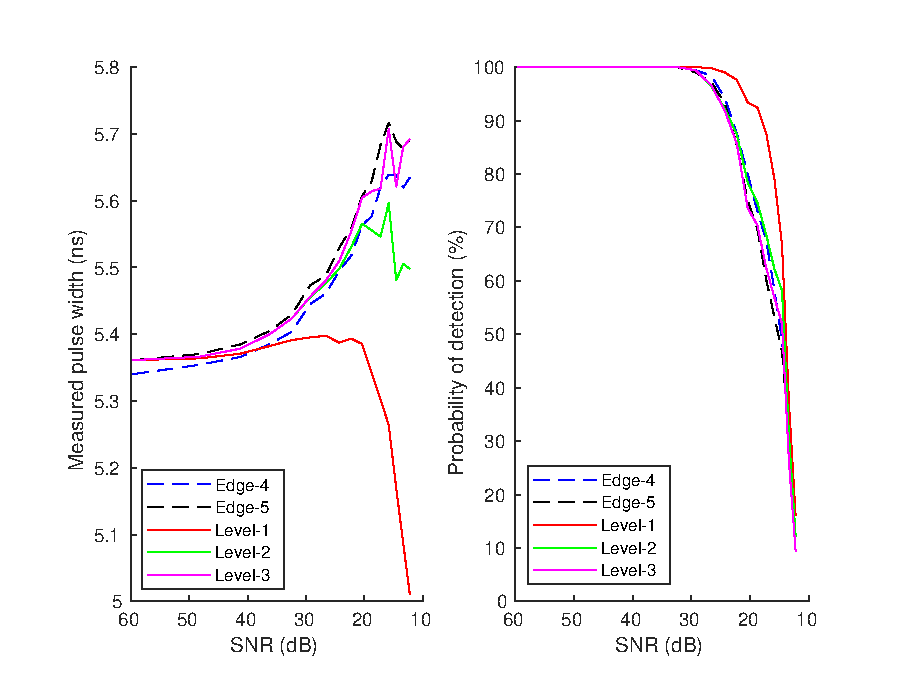
\includegraphics[width=0.8\textwidth]{figures/chapter6_ADC/pd_pw_snr_all.eps}
\caption{Pulse width measurement and Probability of detection}
\label{fig:bm_pw}
\end{figure}
In the figure, the number after the trigger mode indicates the collection-length in $bins$ for edge-triggering and the number of bins of precursor and post-cursor for level-triggering. The result shows that for a particular trigger setting the pulse width increases/decreases with the SNR, and at the same distance (SNR) the pulse width increases with the length (number of bins) of the signal. These trends apply to both edge-triggering and level-triggering. The reason for the trends is that the amplitude of the signal decreases with distance, and the edge-triggering samples a constant length of a signal. Therefore, a larger portion of the leading and falling edge of the signal was captured for a signal from a longer distance, which lowers the \textit{y}-centroid of the signal. Additionally, as the distance increases the leading and falling edge of the signal become noisier, and the noise contributes to a large area at the lower portion of the signal which reduces the \textit{y}-centroid. On the other hand, the measured area under the Gaussian curve remains almost constant as the positive and negative areas induced by the noise were canceled. Therefore, the pulse width increases according to Equation~\eqref{eq:bm_pw}, and more data points captured by the ADC give a longer pulse width. The same reason applies to the edge-triggering as well. Level-3 triggering that captures more data points gives a longer pulse width than the other two. Moreover, as the SNR decreases, the edges of a signal becomes noisier, which results in an increase of the pulse width for Level-2 and Level-3, respectively. An exception is Level-1, which captures the smallest portion of the edges. In this case, the effect of the noise on the pulse width is the minimum. However, on the other hand, the small size of the precursor and the post-cursor truncates the Gaussian pulse, which results in a rise of the \textit{y}-centroid of the signal and therefore, a smaller pulse width. \par
% One should note that even though the pulse width varies with SNR, the difference from  never exceeds the boundaries of the criterion ($$), and if the length of the precursor and post-cursor is selected properly, the pulse width could remain stable in a wide range of distance (Level-1). Moreover, when the SNR is less than $14~dB$, the number above threshold (Metric 1) becomes the decisive factor for the hypothesis determination rather than the pulse width. In other words, the value of pulse width has less effect on the signal determination.  we believe the pulse width metric is valid 
%%%Result: Pd and Pfa
\subsubsection{Probability of detection and  probability of false alarm}
The probability of detection and the probability of false alarm are normally used to evaluate the performance of a detector. The probability of detection is defined as the ratio of the number of signals detected as $\hone$ to the total number of $\hone$ signals, while the probability of false alarm is defined as the percentage of false-positive signals to the total number of noise signals. The probabilities of detection were calculated using the same return signals for the pulse width calculation, and the probabilities of false alarm at different trigger modes and ADC-trigger thresholds were computed using 500 noise signals generated by the noise model with laser pulse turned off. The results are shown in Figure~\ref{fig:bm_pw}(b). From the results we observe that the probability of detection remains greater than $99\%$ at a distance of $100~m$ with an SNR of $30~dB$. The corresponding largest pulse width among the trigger modes is $5.47~ns$ which 
is slightly larger than the upper limit of the criteria. Moreover, all the trigger modes give a probability of false alarm of zero for the ADC trigger at 3x the noise floor and $2\%$ for the trigger at 1x noise floor. Based on the probability of detection and false alarm, we conclude that the detection algorithm that uses the number above threshold and the pulse width of a signal as the metrics demonstrates a high performance on the signal detection for a target distance smaller than $100~m$ (SNR $>30~dB$). For a longer target distance (lower SNR), the increased pulse width reduces the probability of detection. However, if the trigger mode and the length of the precursor and post-cursor is selected properly (\eg Level-1), the distance can be extended to $150~m$ ($23~dB$) with a probability of detection of $99\%$ and $200~m$($19~dB$) with the probability of $92\%$.
% even though the variation of the pulse width at different trigger settings reduces the probability of detection when the SNR decreases, but note that when the SNR is less than $14~dB$ Metric 1 becomes the decisive factor for the hypothesis determination rather than the pulse width.. Consequently, according to the high probability of detection and low false alarm rate at the long distance, we can see the benchmark detection algorithm using the NaT and pulse width gives a good performance of signal detection at least for the distance smaller than $260~m$ (SNR $>14.57~dB$).
%%% Result: Accuracy
\subsubsection{Accuracy and RMS error of distance measurement}
The accuracy (mean error) and the RMS error of the distance measurement using the benchmark estimation algorithm are also evaluated on the 500 observations of the return signal at different distances using both edge and level triggering. The mean error $\overline{\Delta d}$ and the RMS error $\sigma_d$ are defined as
\begin{align}
\overline{\Delta d} = \frac{1}{M}\sum_{m=1}^{M}(d_{meas,m} - d_{GT})\\
\sigma_d = \sqrt{\frac{1}{M}\sum_{m=1}^{M}(d_{meas, m}-\overline{d_{meas}})^2}
\end{align}
where $d_{meas, m}$ is the distance measurement of the $m$-th observation of the total $M$ observations, after converting the measured TOF to distance. $\overline{d_{meas}}$ is the average distance measurement over the $M$ observations for a certain distance and $d_{GT}$ is the corresponding ground-truth distance. The results of the errors are shown in Figure~\ref{fig:bm_error_edge} and Figure~\ref{fig:bm_error_level}.
\begin{figure}[t!p]
\centering
\graphicspath{{figures/}}
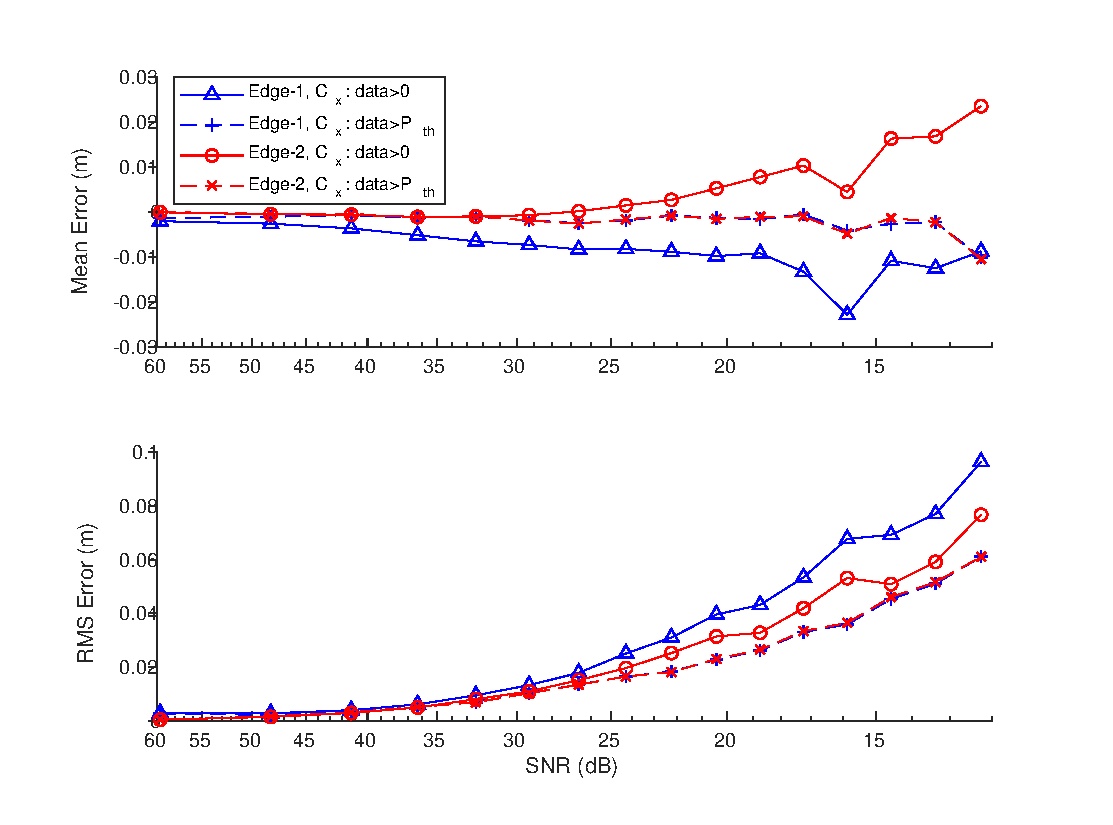
\includegraphics[width=.8\textwidth]{figures/chapter6_ADC/error_snr_edge.eps}
\caption{Mean error and RMS error of distance measurement using edge triggering: edge-1 and edge-2. Distance calculated using data greater than zero is shown in solid lines and using data greater than the ADC threshold is shown in dashed lines.}
\label{fig:bm_error_edge}
\end{figure}%
\begin{figure}[t!p]
\centering
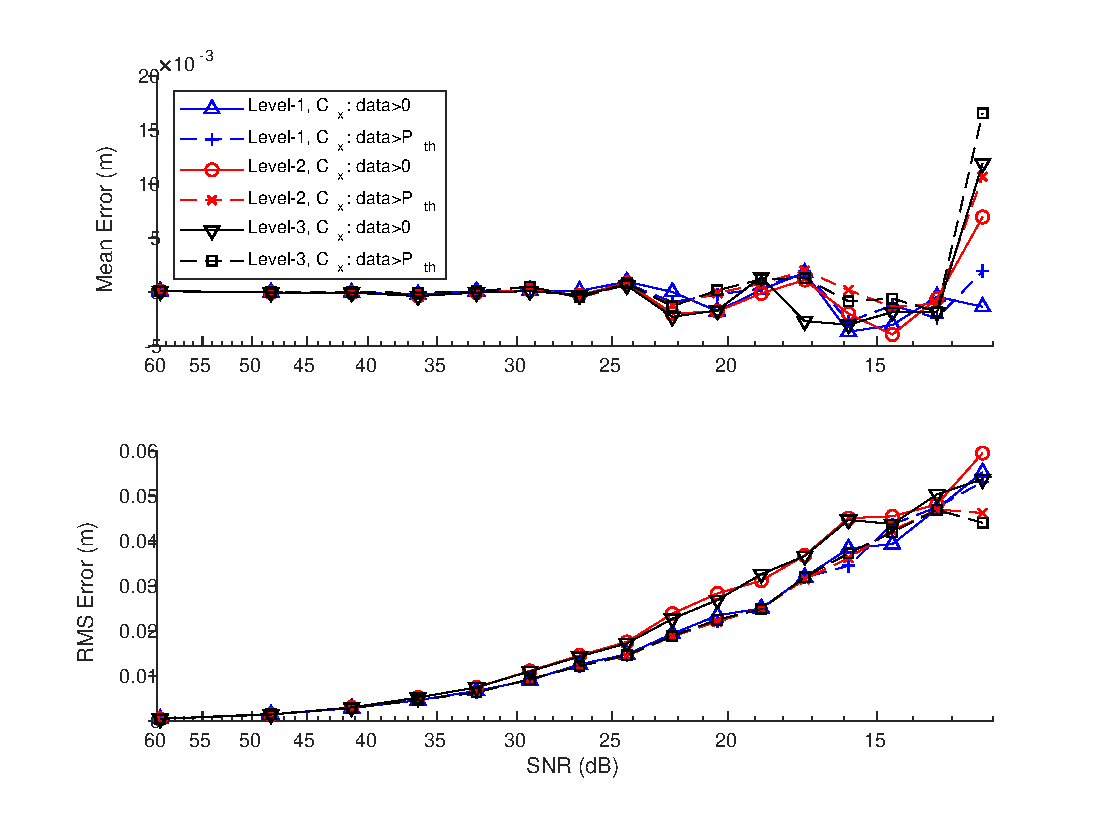
\includegraphics[width=.8\textwidth]{figures/chapter6_ADC/error_snr_level.eps}
\caption{Mean error and RMS error of distance measurement using level triggering: level-1, level-2, and level-3. Distance calculated using data greater than zero is shown in solid lines and using data greater than the ADC threshold is shown in dashed lines.}
\label{fig:bm_error_level}
\end{figure}
%%%
\begin{figure}[t!p] % position options
\graphicspath{ {figures/} }
\centering
    \begin{subfigure}{.7\textwidth}
    \centering
    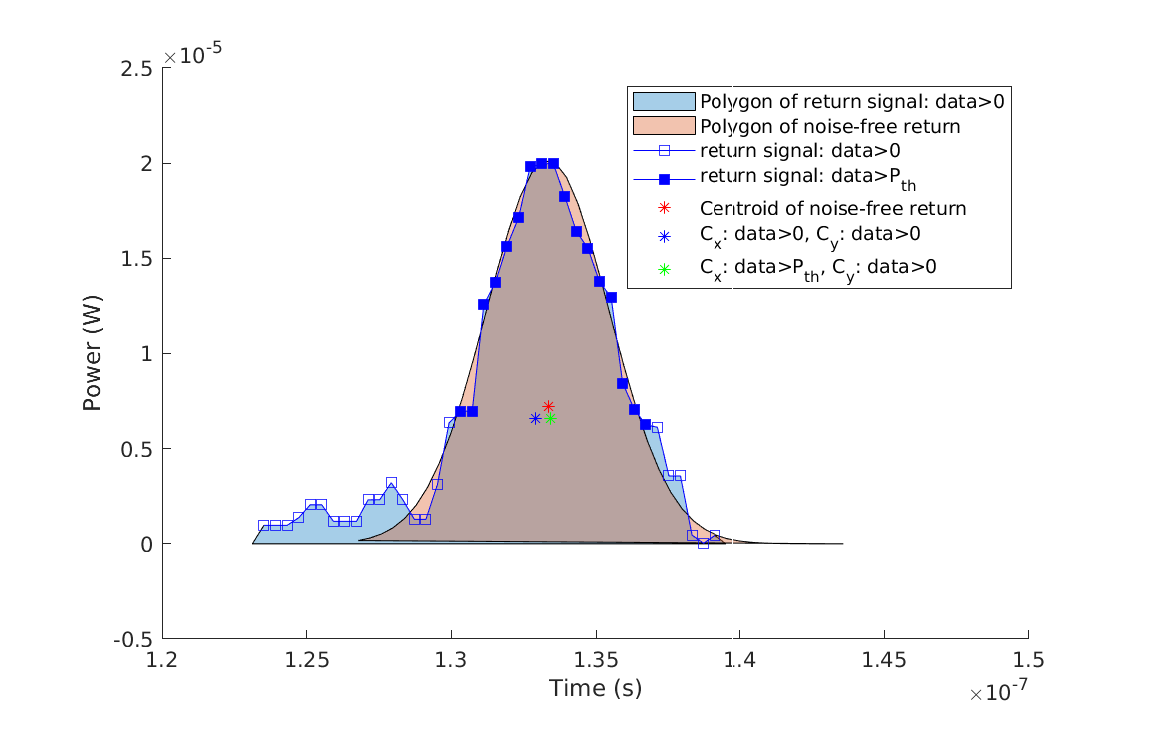
\includegraphics[width=.8\textwidth]{figures/chapter6_ADC/centroid_edge1_d_20_snr20_41.eps}
    % \label{fig:bm_leftshift_edge1}
    \end{subfigure}%
    
    \begin{subfigure}{.7\textwidth}
    \centering
    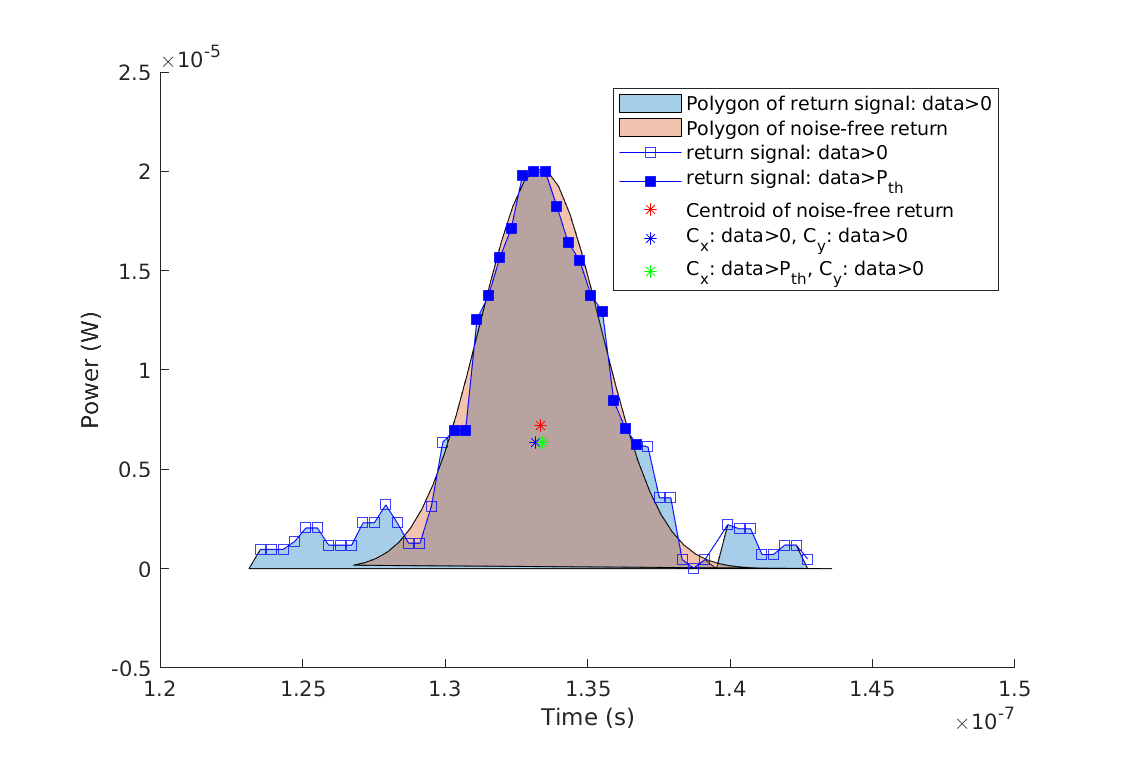
\includegraphics[width=.8\textwidth]{figures/chapter6_ADC/centroid_edge2_d_20_snr20_41.eps}
    % \label{fig:bm_leftshift_edge2}
    \end{subfigure}%
    
    \begin{subfigure}{.7\textwidth}
    \centering
    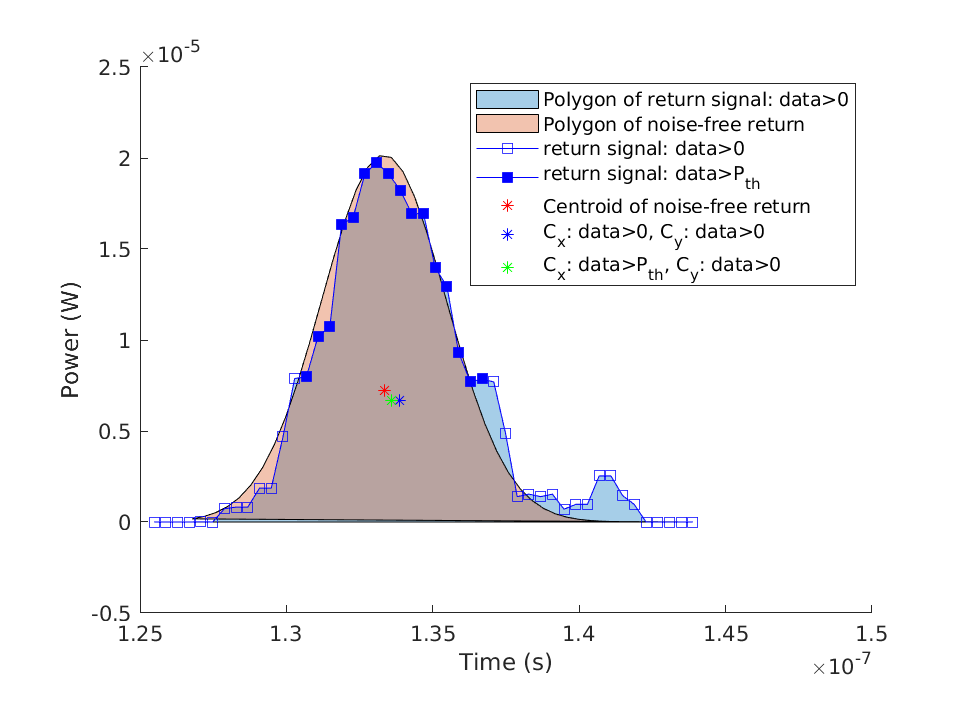
\includegraphics[width=.8\textwidth]{figures/chapter6_ADC/centroid_edge2_d_20_snr20_41_id131.eps}
    % \label{fig:bm_rightshift_edge2}
    \end{subfigure}
    \caption{(a) Left-shift, (b) non-shift (c) right-shift of the \textit{x}-centroid. Case (a) and (b) use the same signal with different trigger settings and Case (c) uses a different signal. The SNR of the signals at all the cases is $20.41~dB$. The trigger settings are (a) Edge-1 (b) Edge-2 and (c) Edge-2.}
     \label{fig:bm_shift}
\end{figure}
From the results, we notice that the mean distance error for the edge triggering using data above zero presents a negative or positive bias. The reason is that at a low SNR the noise on the signal could cause an early triggering on the signal and since the edge-triggering samples a constant length of a signal, a longer leading edge and a shorter falling edge of the signal are captured. The asymmetric signal \wrt the vertical center line of the Gaussian pulse causes the left-shift of the \texttt{x}-centroid and consequently, an earlier arrival time and shorter target distance. Figure~\ref{fig:bm_shift}(a) illustrates the left-shift of the \textit{x}-centroid of the signal. In the figure, the blue star stands for the \textit{x}-centroid using data greater than zero and the red star represents the \textit{x}-centroid of a corresponding noise-free signal. The blue star is shift left to the red star because of the larger portion of leading-edge included in the signal. Setting a longer length of the precursor and post-cursor to cover a longer falling edge could partially reduce the left-shift. An example is shown in Figure~\ref{fig:bm_shift}(b), in which the same signal is sampled by twice the length of the precursor and post-cursor used in Figure~\ref{fig:bm_shift}(a). In this case, the blue star moves closer to the red star. However, since the trigger position on the signal is random and difficult to predict, a longer falling edge could also cause a right-shift of the \textit{x}-centroid and a further target distance (red solid line in Figure~\ref{fig:bm_error_edge} (a)). An example of the right shift of the \textit{x}-centroid is provided in Figure~\ref{fig:bm_shift}(b), in which the blue star shifts to the right of the red star because of the longer falling-edge captured by the ADC.\todo{label figure}\par
Adjusting the length of the precursor and the post-cursor of the edge-trigger is not an optimal solution to the negative/positive bias of the distance measurement due to the randomness of noise. An alternative solution is to use the data above the ADC threshold rather than the data greater than zero. The benefit of using those data points is that most of the data points above the threshold are belong to the Gaussian pulse instead of noise and they have symmetrical distribution around the vertical center line of the pulse. In this case, the \textit{x}-centroid is calculated from symmetric signals. The results of using data above the threshold are shown in the dashed lines in Figure~\ref{fig:bm_error_edge}, which presents a much less bias than the results using the data points above zero. Contrary to the edge-triggering, the positive/negative bias does not appear on the results of level-triggering (Figure~\ref{fig:bm_error_level}(b)). This is because the nature of the level-triggering is to capture the data points above the threshold and symmetric signals are captured for the \textit{x}-centroid calculation.\par
From the results of the RMS error (Figure~\ref{fig:bm_error_edge}(b) and Figure~\ref{fig:bm_error_level}(b)), we can see that for the edge-triggering, covering a larger portion of the pulse balances the fluctuation of the measurement caused by the noise at the leading and falling edge of the signal and yielded a smaller RMS error. However, the length should be chosen with cautions to avoid positive or negative bias on the distance measurement. On the contrary, a smaller size of the precursor and post-cursor for the level-triggering reduces the effect of noise on the centroid measurement and improves the measurement accuracy. The RMS error using data greater than zero and data above the ADC threshold are also compared, and the former one gives a larger RMS error, which is because the noise included in the signal causes a larger fluctuation that the later one on the \textit{x}-centroid measurement and the distance measurement.


% suggestoni: capture large enough portion of the gaussian shape, but least noise


% result1: accuracy and std, pd vs SNR for edge, level-8 and level-16.
% discussion on accuracy (level and edge) : left and right shift
% discussion on pd: how # and pd changes with SNR, show polygon plots.

% results 2: after AFE, check how pw changes
% results 3: different kind noises
% pw variance with SNR
% error vs SNR, pfa and pd vs SNR, ROC, 
% different noises on error, pfa, pd ...
% measurements on real data


\chapter{Time Discrimination-ADC -  Neyman-Pearson Detector}\label{ch:NP}
The Neyman-Pearson(NP) detector was first introduced by Jerzy Neyman and Egon Pearson in 1933\citep{neyman1933problem}, and it has been proven to be the optimal detector for radar/ laser signal detection \cite{kay1998fundamentals}. \todo{add the review to background section} 
% and has been widely utilized in many applications like target detection, medicine, nuclear energy, gravitational-wave astronomy, \etc\cite{Hoover2000LocatingResponse,Bousselham2007SamplingTiming,seto2001possibility,gronwall2007influence,gu2002detecting,Jordan2009RangeData,roman2000parametric,Ofek2017OptimalDetection,Vio2018MatchedImplementation}. 
In general, the NP detector conducts a likelihood ratio test(LRT) to detect a known deterministic signal, \ie the signal has no unknown parameters, while in our case, the arrival time and the amplitude of the return pulse are unknown. In that case, a generalized likelihood ratio test(GLRT) is utilized for detection of signals that have unknown parameters. Moreover, the arrival time of signals can also be determined in the detection process, so our signal detection and estimation problem are combined together, and the problem is defined in the next.
%% problem definition
\section{Problem definition}
We state the signal $x[n]$ collected by an ADC is composed of a Gaussian distributed white noise under hypothesis $\hzero$, and under hypothesis $\hone$ the signal is the summation of the noise-free return pulse with unknown amplitude, $As[n]$, and white noise following a  Gaussian distribution. Symbolically,
\begin{align}\label{eq:mf_hypothesis}
\mathcal{H}_0:x[n]&=w_0[n]  &n=0, 1,\ldots, N-1\\
\mathcal{H}_1:x[n]&=As[n-n_0]+w_1[n]  &n=0, 1,\ldots, N-1    
\end{align}
where $w_0$ and $w_1$ are the white noise under $\hzero$ and $\hone$ with the variance $W$, and $s$ is the template of the transmit signal normalized to unit amplitude which is also called 'kernel'. The kernel is scaled by the unknown amplitude $A$ and it is assumed to be nonzero over the time interval $[0,M-1]$. The index $n$ represents the timestamp of the $n$-th point of the signal with a size of $N$, and $n_0$ stands for the arrival time of the signal. The time period $[0, N-1]$ should cover the signal for all the possible arrival time, \ie $n_0\in[0, N-M]$. \par
Note in Equation \eqref{eq:mf_hypothesis}\todo{change eq No.}, the noise on each point of a signal is approximated to be Gaussian distributed, even though the shot noise is created with a Poisson distribution. This approximation is explained in \citep{wall1979practical} who states that, despite the number of photons follows Poisson statistics, after sufficient integration for a photon detector of more than 10 photons per integration time interval, the distribution is reduced to Gaussian. In our case, the collected number of photons is far beyond 10 when the laser is on, so the Gaussian approximation is valid. In addition, the white noise $w_0$ and $w_1$ usually have different variances because the shot noise induced by the laser pulse also contributes to the variance of $w_1$. However, the $W_1$ is usually unavailable since the pulse-induced shot noise is amplitude depended which is unknown, and the unknown amplitude also makes it difficult to measure the variance of the pulse-induced shot noise with the appearance of the pulse. Therefore, in this study the $w_0$ and $w_1$ are assumed to be identical, denoted by $w$, and they share the same variance $W$. Also. we can see this approximation does not affect the PFA, and has negligible influence on the PD in next few sections. \par
Next, we introduce the Neyman-Pearson theorem which allows us to decide the hypothesis of a signal.
% NP theorem
\subsection{Neyman-Pearson Theorem}
The Neyman-Pearson theorem (NP theorem) states that, to maximize the probability of detection (PD) $P_D$ of a signal for a given probability of false alarm (PFA) $P_{fa}  =\alpha$, decide $\mathcal{H}_1$ if the generalized likelihood ratio $L_G(x)$ is greater than a threshold $\gamma$; otherwise, decide $\mathcal{H}_0$:
\begin{equation} \label{eq:Lx}
L_G(x)=\frac{p(\vec{x};n_0,A,\mathcal{H}_1)}{p(\vec{x};\mathcal{H}_0)}\underset{\mathcal{H}_0}{\overset{\mathcal{H}_1}{\gtrless}}\gamma
\end{equation}
The threshold $\gamma$ can be derived from the definition of the PFA
\begin{equation}\label{eq:pfa}
P_{fa}=\int_{\{\vec{x}:L_G(x)>\gamma\}} p(x;\mathcal{H}_0)dx=\alpha,
\end{equation}
and the PD can be obtained by:
\begin{equation} \label{eq:pd}
P_D=\int_{\{\vec{x}:L_G(x)>\gamma\}}p(x;n_0, A, \mathcal{H}_1)d\vec{x}
\end{equation}
The probability density distribution (PDF)  of signals with unknown parameters $n_0$ and $A$ under hypothesis $\hzero$ and $\hone$ are denoted by $p(\vec{x};n_0, A,\mathcal{H}_1)$ and $p(\vec{x};\mathcal{H}_0)$, respectively, and the vector $\vec{x} = [x[0],x[1],...,x[N-1]]$. The generalized likelihood ratio indicates the likelihood of a signal being $\hone$ versus being $\hzero$, and Inequation \eqref{eq:Lx} is called the generalized likelihood ratio test. After mathematical reorganization, the GLRT is reduced to (the derivation is provided at the end of this chapter.\todo{ref the last page of this chapter}):
\begin{eqnarray} \label{eq:Tx}
T(x) &=&\sum_{n=n_0}^{n_0+M-1}x[n]s[n-n_0] \underset{\mathcal{H}_0}{\overset{\mathcal{H}_1}{\gtrless}}\gamma'\\
\gamma'&=&\frac{A}{2}\sum_{n=0}^{M-1}s^2[n]+\frac{W\ln\gamma}{A}
\end{eqnarray}
and Equation\eqref{eq:pfa} is reformed to
\begin{equation}\label{eq:pfa2}
P_{fa}=Pr(T(x)>\gamma';\mathcal{H}_0)
\end{equation}
where $T(x)$ is the test statistic which needs to be calculated from experiments. Equation\eqref{eq:Tx} indicates the GLRT calculates the cross-correlation of the signal $x$ with the kernel $s$ for all possible $n_0$, and compares the maximum value with the threshold $\gamma'$. If the threshold is exceeded, a pulse is claimed to be present, and the arrival time $n_0$ is equal to the timestamp of the maximum value. Otherwise, noise is claimed detected. Mathematically, the test statistic can also be written as
\begin{align}\label{eq:MF_Tx_argmax}
    T(x)&=\max_{n_0\in[0,N-M]}\sum_{n=n_0}^{n_0+M-1}x[n]s[n-n_0]\\
    n_0&= \argmax_{n_0\in[0, N-M]}T(x)
\end{align}
In practice,  $T(x)$ can be obtained from the convolution of a signal with the conjugated time-reversed kernel $s'[n]$, \ie for each timestamp $n$, the convolution result is
\begin{align}\label{eq:MF_conv}
y[n]&=\sum_{m=0}^nx[m]s'[n-m]\\
s'[n]&=s[N-1-n]
\end{align}
and Equation\eqref{eq:MF_conv} is also known as the \emph{matched filter} (MF). For simplicity, this detection algorithm is called NP detector in this work. The NP detector is proved mathematically equivalent to the correlation between the signal and the kernel. For the difference between the correlation approach and the NP detector readers could refer to [Kay, book]\todo{add kay book Vol II}for details.
\subsection{Fast Fourier Transformation Approach}
The NP detector can be achieved by sliding the kernel over an input signal in time domain. The time complexity of the temporal convolution approach can be denoted by $\mathcal{O}(MN)$ in which $M$ and $N$ are the number of points of the kernel and the signal, respectively. Therefore, the MF could be computationally intensive if the signal contains a large number of data points. Alternative solution is needed to accelerate the computation. As we know that the convolution of two signals in time domain is equivalent to a dot product of the Fourier Transformation of the two signals in frequency domain, the Equation~\eqref{eq:MF_conv} can be implemented in frequency domain by using Fast Fourier Transformation (FFT). Specifically, 
\begin{align}
X&=\mathcal{F}[x]\\
S&=\mathcal{F}[s]\\
Y&=X\cdot S\\
y&=\mathcal{F}^{-1}[Y]
\end{align}
where the variable $X$, $S$, and $Y$ are the Fourier Transformation (FT) of the signal $x$, $s$ and $y$ in frequency domain, and the symbol $\mathcal{F}$ and $\mathcal{F}^{-1}$ are the FT and inverse-FT operators. The time complexity of an FFT operation is $\mathcal{O}(N\log N)$ which is much smaller than $\mathcal{O}(MN)$. Another benefit of using FFT is that arrival time smaller than the ADC sampling interval can be resolved by using zero-padding technique. In other words, the temporal resolution of the convolution results can be improved.\ par
The zero-padding technique is to add zeros to signals in time or frequency domain), and the sampling rate of signals in frequency or time domain increases after FT or inverse-FT. For an FFT operation without zero-padding, since the number of points in frequency domain is equal to the number of data points used in the FFT in time domain, the resolution of the signal is unchanged, \ie no improvement is on the resolution. On the contrary, for a signal having $N$ points (sampling rate of $1/N$) in time domain, if $N$ zeros are padded at the end of the signal in frequency domain (assuming the frequency is centered around zero), the signal will have $2N$ points after inverse-FT. And since the time range is unchanged, the resolution of the signal is doubled. On the other hand, the FFT is most efficient when the number of points of a signal is an integer power of two, which means zero padding in time domain is also needed for signals have variable sizes, and note that the time-domain zero-padding only extends the length of the signal but does not increase the signal resolution. In this work, we first zero-pad the signal $s$ and $x$ to an identical length $L_{p2}$ which is the smallest power of two of the total length ($M+N-1$) of the two signals. After FFT, we add $K$ zeros to the dot-product result $Y$, and $K$ is an integer times the length $L_{p2}$. After the zero-padding in frequency domain, the size of the resultant signal is extended to $(K+1)L_{p2}$, and then the resultant signal is converted back to time domain and the size of the signal is unchanged. The convolution result $y$ has additional zeros which results from the time-domain zero-padding at the first step, so the zeros are removed from the convolution result. After the zero-removal, the size of the convolution result becomes $(K+1)(M +N-1)$, \ie the resolution increases $K+1$ times than the sliding-window convolution. Accordingly, the original time interval $\Delta t$ is reduced to $\Delta t/(K+1)$. Note that the size of the convolution result is larger than the time series, so only the center portion of the convolution result is kept to maintain the size consistency. An example of the zero-padding in time domain and in frequency dodfdffmain is shown in Figure ~\ref{fig:ADC_NP_zeropad}. The time is arbitrary. In Figure~\ref{fig:ADC_NP_zeropad} (c), we can see the resolution of the convolution result is double after frequency-domain zero padding.
\begin{figure}[t!p]
\centering
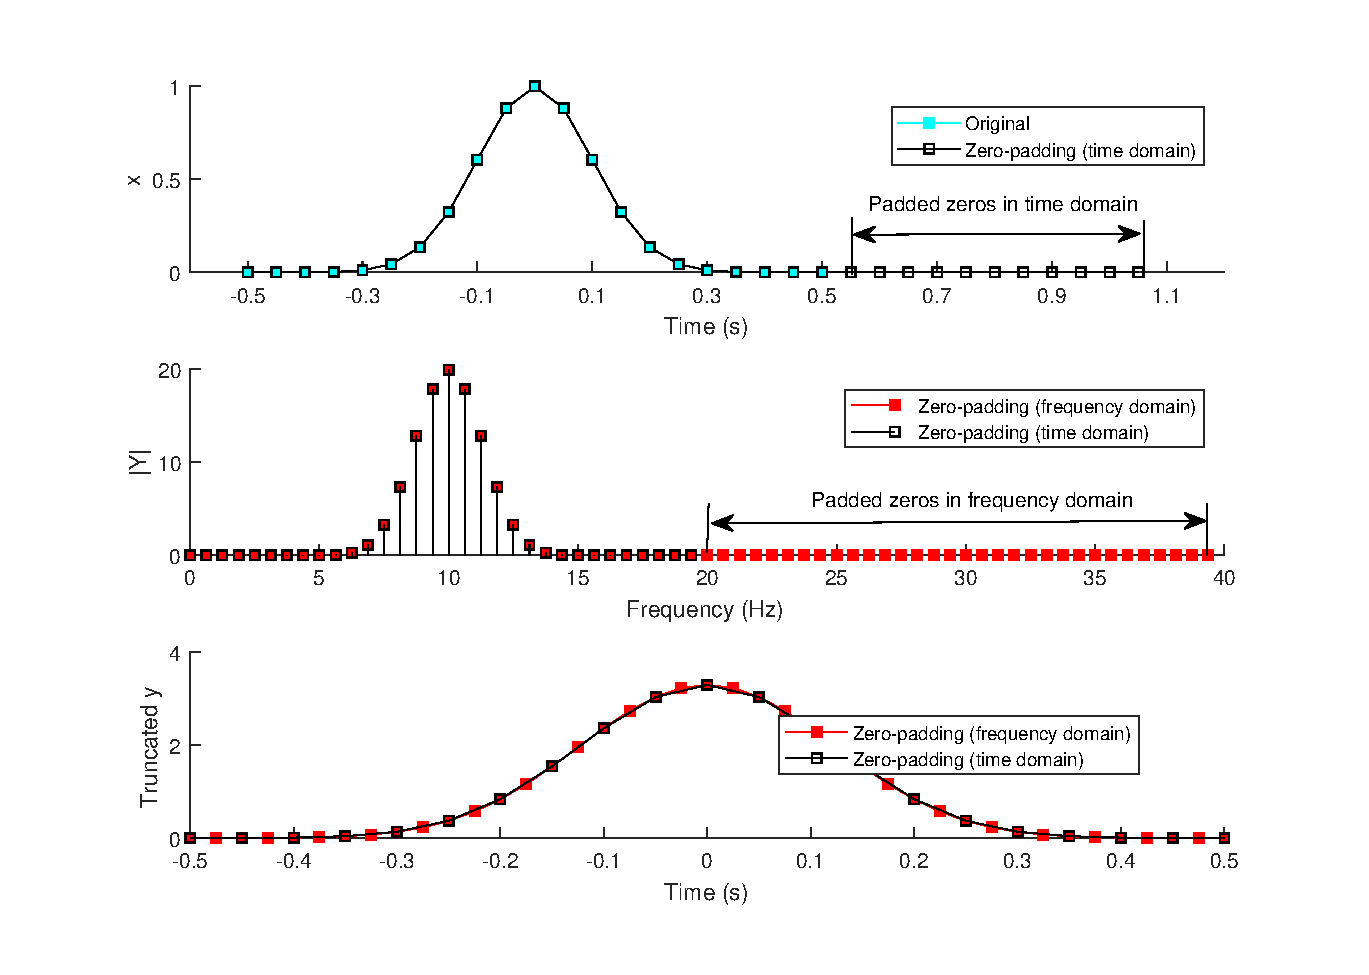
\includegraphics[width=0.8\textwidth]{figures/chapter_ADC_MF/signal_pad_nopad.eps}
\caption{Example of zero-padding in time domain and frequency domain}
\label{fig:ADC_NP_zeropad}
\end{figure}
% PDF
\subsection{PDF of $T(x)$}
Now, the original GLRT (Equation \eqref{eq:Lx}) is reduced to a problem that compares the $T(x)$ with a new threshold $\gamma'$ (Equation\eqref{eq:Tx} and Equation \eqref{eq:MF_Tx_argmax}). Now, we need to determine the threshold $\gamma'$ using Equation \eqref{eq:pfa2} for a given $P_{fa} = \alpha$, for which the PDFs of $T(x)$ under both hypothesis $\hzero$ and $\hone$ are required. Since $T(x)$ is a linear combination of Gaussian distributed variables, the PDFs of $T(x)$ should also follow a Gaussian distribution. The estimation of the mean $\hat{\mu}$ and the variance $\hat{\sigma}^2$ for hypothesis $\hzero$ and $\hone$ are shown below, of which the derivation is given at the end of this chapter\todo{refer to last page of the chapter}:
\begin{align} \label{eq:pdfTx}
\hat{\mu_0}&=0\\
\hat{\sigma_0^2}&=W\sum_ns[n]^2\\
\hat{\mu_1}&=A\sum_ns^2[n]\\
\hat{\sigma_1^2}&=W\sum_ns^2[n],
\end{align}
and the PDFs of $T(x)$ follow:
\begin{align}
\mathcal{H}_0: & T(x)\sim N(\hat{\mu_0}, \hat{\sigma}_0^2)\\
\mathcal{H}_1: & T(x)\sim N(\hat{\mu_1}, \hat{\sigma}_1^2)
\end{align}
Or, the normalized test statistic $T'(x) = \frac{T(x)-\hat{\mu}}{\hat{\sigma}^2}$ follows the standard normal distribution $\mathcal{N}(0,1)$.
% threshold
\subsection{Estimation of threshold $\gamma'$}
Having the PDF of $T(x)$, Equation \eqref{eq:pfa2} can be expressed by
\begin{align} \label{eq:pfa_gamma}
\begin{split}
P_{fa}&=Pr(T(x)>\gamma';\mathcal{H}_0)\\
&=Pr(T'(x)>\frac{\gamma'-\hat{\mu}_0}{\hat{\sigma}_0};\mathcal{H}_0)\\
& = Q(\frac{\gamma'-\hat{\mu}_0}{\hat{\sigma}_0})
\end{split}
\end{align}
where 
\begin{align}
\begin{split}
Q(x) &=\int_x^\infty\frac{1}{\sqrt{2\pi}}\exp(-\frac{1}{2}t^2)dt\\
&=\frac{1}{2}[1-erf(\frac{x}{\sqrt{2}})]\\
&=\frac{1}{2}erfc(\frac{x}{\sqrt{2}})\\
&=1-\Phi(x)
\end{split}
\end{align}
and $\Phi(x)$ is the cumulative distribution function(CDF) for a standard normal distributed variable, and $Q(x)$ is the complementary cumulative distribution function(CCDF). Then, we can derive the expression of $\gamma'$
\begin{align} \label{eq:MF_gamma'}
\gamma'=\hat{\sigma}_0Q^{-1}(P_{fa})+\hat{\mu}_0    
\end{align}
Here, we can see the PFA is not a function of the amplitude $A$ or the variance of $\hone$signal $w_1$, which means the amplitude of a signal and the variance will not affect the FPA. However, the PD could be affected. The theoretical PD can be obtained from \eqref{eq:pd}
\begin{align}
\begin{split} \label{eq:MF_pd}
P_d&=Pr(T(x)>\gamma';n_0,A, \mathcal{H}_1)\\
&  = Pr(T'(x)>\frac{\gamma'-\hat{\mu}_1}{\hat{\sigma}_1};n_0,A, \mathcal{H}_1)\\
& = Q(\frac{\gamma'-\hat{\mu}_1}{\hat{\sigma}_1})\\
&=\frac{1}{2}erfc(\frac{\gamma-\hat{\mu}_1}{\sqrt{2}\hat{\sigma_1}})
\end{split}
\end{align}
Plugging Equation \eqref{eq:MF_gamma'} in Equation \eqref{eq:MF_pd}, we have
\begin{align} \label{eq:MF_deflectCoef}
P_d &= Q(Q^{-1}(P_{fa})-\sqrt{d^2})\\    
d^2 &= \frac{A^2s^2[n]}{W}
\end{align}
where $d^2$ is the deflection coefficient, which can be interpreted as the normalized difference between the PDF of $T(x)$ under hypothesis $\hone$ and hypothesis $\hzero$ by the variance of the noise. The deflection coefficient illustrates that the separation between the two PDFs, as shown in the schematic Figure \ref{fig:dsquare}. In the case of the deflection coefficient is large, the position of the threshold has less impact on the PD, and the detector is approaching a perfect detector($PD = 1$). However, as shown in Equation \eqref{eq:MF_deflectCoef} the deflection coefficient is a function of the amplitude $A$ and variance $W$of a signal, which means the smaller amplitude and larger variance could move the two PDFs closer which causes a decrease of PD.
\begin{figure}[t!p]
\centering
\includegraphics[width=.8\textwidth]{figures/chapter6_ADC/dsquare.jpg}
\caption{PDF of $\hzero$ and $\hone$, and the deflection coefficient [Ref [Kay book]]}
\label{fig:dsquare}
\end{figure}
% Procedure
\subsection{Procedure of the NP detector}
Now, we have the problem defined and also the PDFs and the threshold derived. To summarize, the procedure of the NP detector for the signal detection and estimation is following:
\begin{enumerate}
\item Find the kernel $s[n]$;
\item Find the STD of noise $x[n]$;
\item Calculate the PDFs of the test statistic T(x): Equation \eqref{eq:pdfTx}; \todo{change equation label}
\item Calculate the threshold $\gamma'$ (threshold for $T(x)$): Equation\eqref{eq:MF_gamma'};
\item Calculate the $T(x)$ over all possible $n_0$ by convoluting the input signal $x$ and the kernel $s$, and find the maximum value of $T(x)$ and the corresponding $n_0$: Equation\eqref{eq:MF_Tx_argmax} and Equation \eqref{eq:MF_conv};
\item Compare the maximum value of $T(x)$ with the threshold $\gamma'$, and decide the hypothesis of the signal: Equation \eqref{eq:Tx};
\item If $\hone$, estimate the arrival time $n_0$: Equation \eqref{eq:MF_Tx_argmax}.
\end{enumerate}
%% Application to simulated signals 
\section{Application to simulated signals}
In this section, the application of the MF to noise signals and pulse signals was studied. The experiment design will be introduced first followed by the results and discussion.\par
\subsection{Study cases}
A case with pure noise signals and one with noisy return pulses were studied in this work. For both cases, the ADC threshold was set 3x noise floor above zero, and the edge-trigger model with a precursor length of 1 and collection length of 5 was used. More details of the two cases are explained below.
\subsubsection{Case 1: Noise (laser is off)}
For the case of noise, 1000 observation of pure noise signals (with lase turned off) were generated by the noise model with a sampling rate of 100GHz as suggested in the Pulse Model section. In the noise model, the background and dark-current induced shot noises were at first generated at each data point following a Poisson distribution and then smoothed by a moving average with a kernel size of 5. The moving average is to model the APD integration process, and the size of 5 is determined by the integration time of the APD. The APD used in this study has a bandwidth of 10GHz, so the integration frequency is 2x10GHz (the integration time is 1/20GHz or 0.05ns), which results in the size of 5 for the averaging window. Next, the noise signals were subsampled with a rate of 2.5GHz to model the sampling process of an ADC with a sampling rate of 2.5GHz for the two-channel mode. 
\subsubsection{Case 2: Pulse}
Return signals reflected from targets at different distances were tested for the case with the laser on. The distance ranges from 5m to 60m with an increment of 5m and the corresponding SNR ranges from 44.4dB to 1.27dB. For each distance, 1000 return signals were generated by the pulse model, the propagation model, and the noise model. The process of moving averaging and subsampling is the same as in Case 1. 
% Detection and Estimation Algorithm: NP detector (MF) 
\subsection{Detection and Estimation Algorithm: NP detector (MF)}
The NP detector was used for the signal detection and TOF calculation. The kernel of the NP detector was obtained from the pulse model with the amplitude normalized to one. The PFA is set to 0.001 which is a typical value for a laser range finder \citep{burns1991system}. In Case 1, the variance $W$ is calculated dynamically from each observation, meaning the threshold is dynamic for the MF. In Case 2, as mentioned in Section (principle section), the variance $\sigma^2_1$ is assumed to be equal to $\sigma^2_0$, \ie $\sigma^2_1= \sigma^2_0 = W$. The PDFs of the $T(x)$ and the threshold can be obtained from Equation \eqref{eq:pdfTx}.
% % Discussion
\subsection{Results and Discussion}
\subsubsection{Threshold}
The threshold for the MF is determined by the STD of the $\hzero$ signals, $\sigma^2_0$, and different ways of calculating the STD results in different PFAs. The STD of noise signal can be obtained from the datasheet of an electronic device or measurement of an oscilloscope or signals collected by an ADC. A comparison of the STD obtained from signals before ADC sampling (analogy to oscilloscope measurements) and after sampling (analogy to signals collected by an ADC) is shown in Figure 1. The figure shows the before-sampling signals have a smaller STD compared to after-sampling signals, which results in a lower threshold, and consequently a high PFA. The reason for the difference of the STD is that the ADC only samples a limited number of data points from analog signals, and the variance of the subset of a signal is usually higher than the one of the analog signals. Consequently, the threshold for a given PFA is underestimated by using the STD of before-sampling signals. Therefore, to achieve the given PFA, the STD of the $\hzero$ signals should be calculated from the signals collected by an ADC, rather than before the ADC sampling, from oscilloscope measurements or the datasheet of an electronic device. 
% Figure 1 The STD of 1000 noise signals before ADC sampling (red) and after ADC sampling (blue).
\subsubsection{Probability of false alarm}
Monte-Carlo experiment was performed on 100 tests, each of which contains 1000 observations. The PFA of each test was measured the average PFA was obtained by averaging over the PFAs of the 100 tests. The resultant $P_{FA,aveg} $is equal to 0.08 with an STD of 0.025. The measured PFA is higher than the predefined value (0.001) because the defined threshold is for an LRT on signals with known arrival time, but the arrival time is unknown in our study. Therefore, a convolution over the entire signal is required, in which case the random noise on the signal has a much higher probability to exceed the threshold and be detected as a pulse.
\subsubsection{Probability of detection}
All the signals in Case 2 give a $P_D=1$. This is because even though the PD is theoretically dependent on the amplitude of the signal Equation \eqref{eq:MF_deflectCoef}, the deflection coefficient is large, even for signals with a low SNR. A signal observation with an SNR of 1.31dB is shown in Figure 2 along with the convolution results and the threshold. In the example, the square root of the deflection coefficient ($d = 15.7$) is much larger than the normalized threshold ($\gamma '/\sigma_0 = 3.09$), which means the PDF of hypothesis $\hone$ is separated from the one of hypothesis $\hzero$. One can also use the MLE to estimate the amplitude of the signal to reduce the effect of the amplitude on the PD \citep{kay1998fundamentals}: 
\begin{equation}
    A =\frac{\sum_{n=0}^{N-1}x[n]s[n]}{\sum_{n=0}^{N-1}s^2[n]}
\end{equation}
However, since the PD is already equal to 1 in our case, the MLE estimation is skipped, but it could be an option for readers who have situations that have a smaller amplitude, and a high PD is requested.
% Figure 2 Simulated signal with an SNR of 1.31dB with its convolution result and threshold. The maximum value of the convolution result is still higher than the threshold
\subsubsection{Accuracy and Precision}
The mean error and the RMS error are calculated to evaluate the performance of the MF. Both the sliding-window and the FFT approaches were applied. Also, to reduce the effect on the noise on the measurement, a Butterworth low-pass filter with cutoff frequency of 0.4GHz and sampling rate of 2.5 GHz was applied \todo{more details of the LP filter will be given in Section xx},The results are shown in Figure~\ref{fig:error_NP_sim}. 
 \begin{figure}[t!p]
\centering
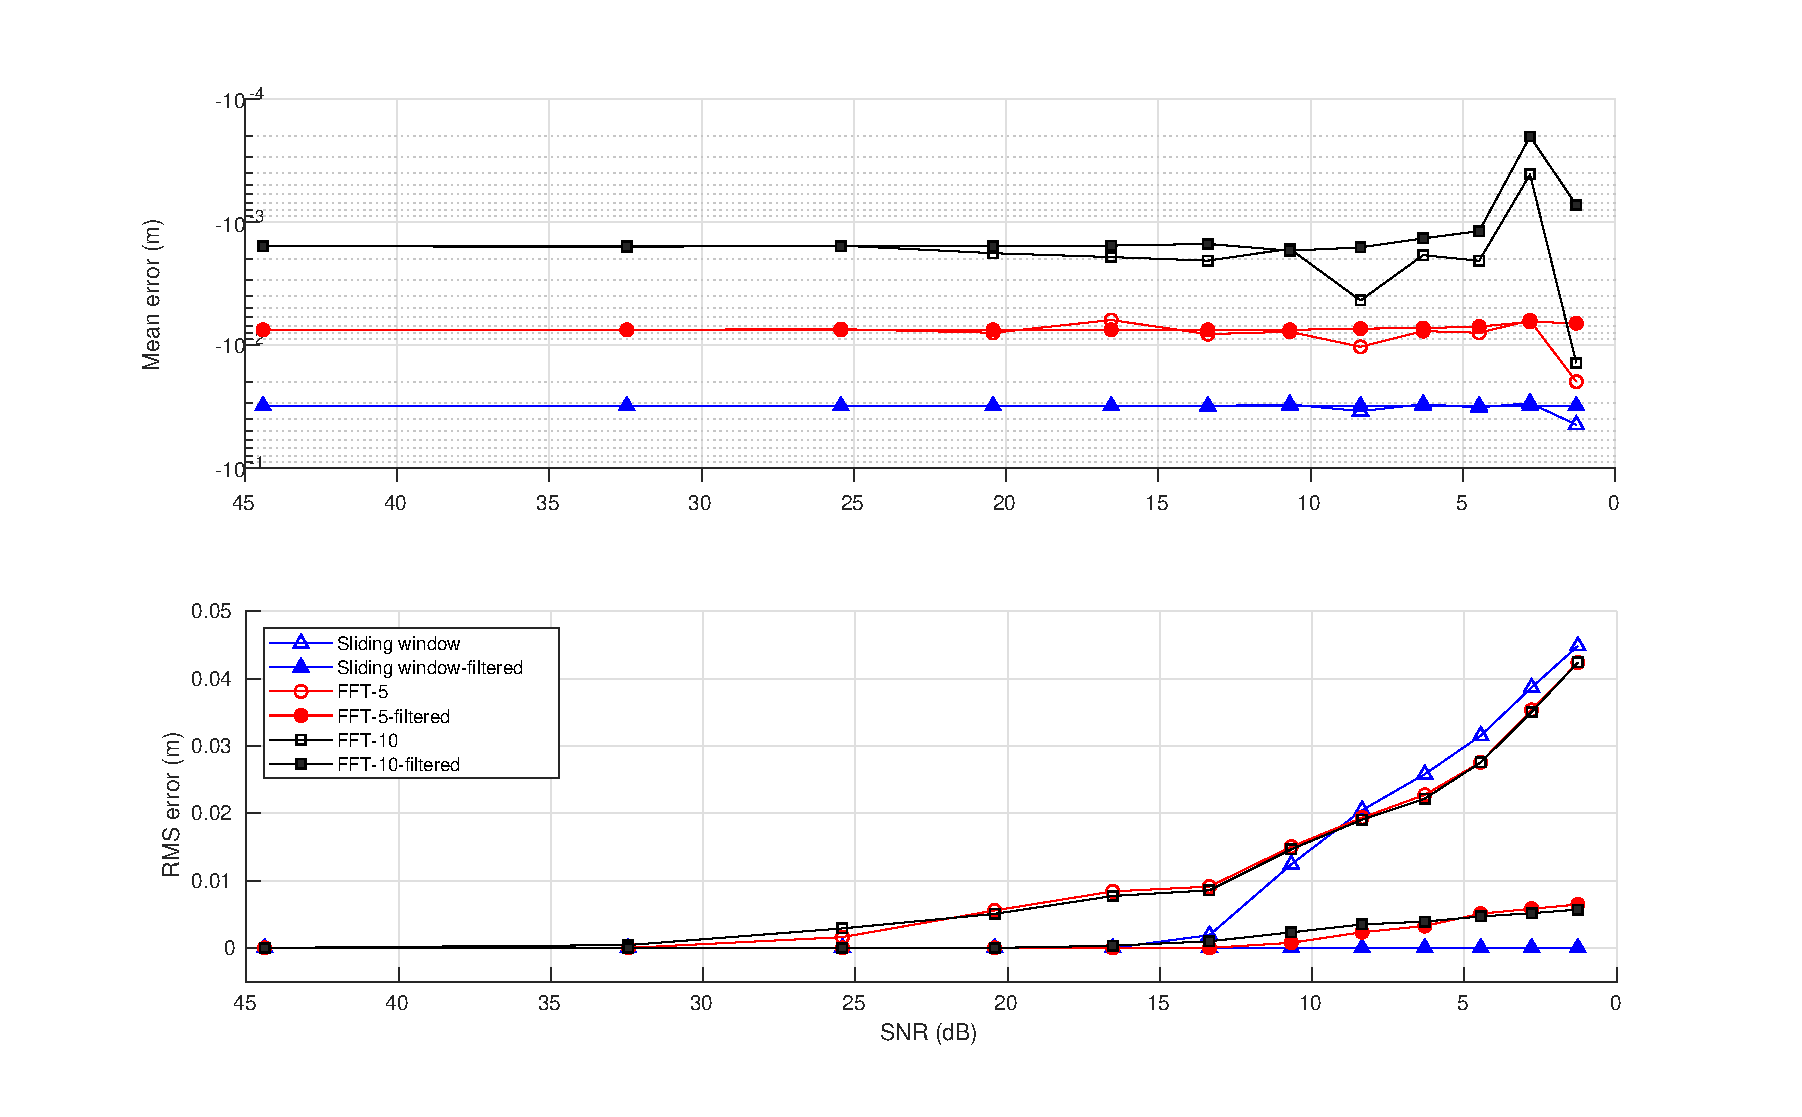
\includegraphics[width=1\textwidth]{figures/chapter_ADC_MF/Error_convVsFFT_filt_unfilt_sim.eps}
\caption{Mean and RMS error of the NP detector using the SW and FFT approaches. The number after FFT indicates the times the resolution is refined. The hollow marker indicates the results without filtering, and the solid marker denotes the result after filtering}
\label{fig:error_NP_sim}
\end{figure}
From the result of the Mean error, we can see the sliding window approach has a larger error than the FFT approach, and larger number of zero-padding gives better accuracy. The reason is that the Mean error is affected by the resolution of the signal. The sliding-window approach has the coarsest resolution, so any errors caused by the noise is at least 0.4 ns (0.06m). On the contrary, the FFT-approach refines the resolution 5 and 10 times than the sliding-window approach, which results in a less Mean error and the FFT-10 provides the least Mean error. Additionally, the LP-filtering slightly reduces the Mean error for long distance. The comparison of the effect of the resolution on the measurement accuracy between different approaches is given in Figure~\ref{fig:NP_sig_FFT5} and Figure~\ref{fig:NP_sig_FFT10}. From the figure we can see because of the finer resolution, the peak position of FFT-10 is closer to the ground-truth position than FFT-5, and the peak position of the sliding-window approach has the largest separation from the ground-truth. \par
\begin{figure}[t!p]
\centering
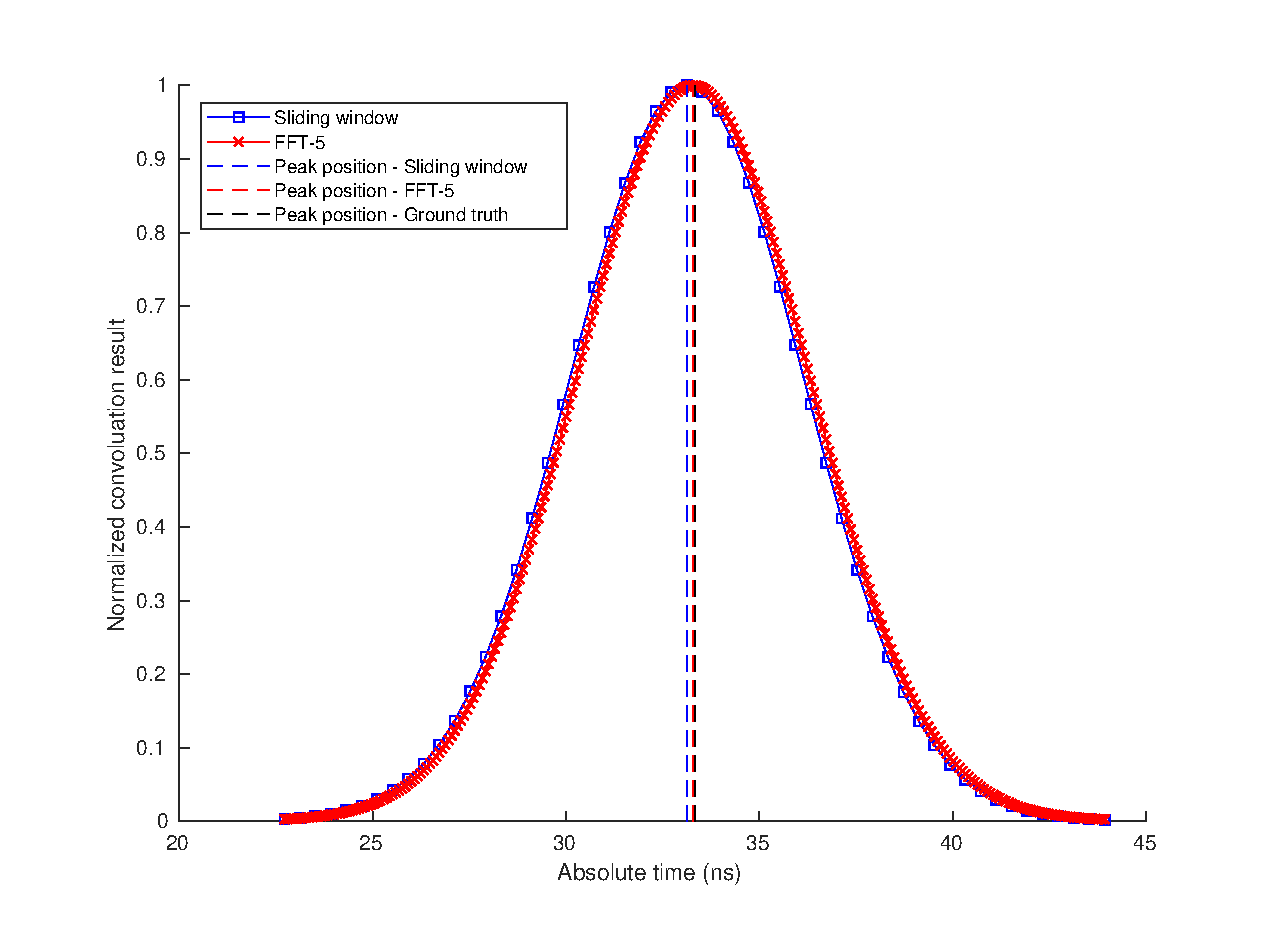
\includegraphics[width=1\textwidth]{figures/chapter_ADC_MF/plot_convRes_FFT5_sim.eps}
\caption{Convolution result of FFT-5}
\label{fig:NP_sig_FFT5}
\end{figure}
%
\begin{figure}[t!p]
\centering
\includegraphics[width=1\textwidth]{figures/chapter_ADC_MF/plot_convRes_FFT5_zoomin.eps}
\caption{Convolution result of FFT-5 zoom in}
% \label{fig:NP_sig_FFT5}
\end{figure}
%
\begin{figure}[t!p]
\centering
\includegraphics[width=1\textwidth]{figures/chapter_ADC_MF/plot_convRes_FFT10_sim.eps}
\caption{Convolution result of FFT-10}
\label{fig:NP_sig_FFT10}
\end{figure}
%
\begin{figure}[t!p]
\centering
\includegraphics[width=1\textwidth]{figures/chapter_ADC_MF/plot_convRes_FFT10_zoomin.eps}
\caption{Convolution result of FFT-10 zoom in}
% \label{fig:NP_sig_FFT10}
\end{figure}
From the RMS error, we notice that the sliding-window has a better precision than the FFT-approaches for shorter distance, but the precision becomes worse as the distance increases. The difference is also caused by the resolution of the result. At short distance, the signal is less noisier and the samples of a signal are more separated for the sliding-window approach than the FFT's, so the peak of the convolution result is less challenged by the adjacent points, which results in smaller variation of the time(distance) calculation. On the contrary, the samples at the top portion of the signal are likely have similar values for the FFT approaches, due to the smaller separation between the sample points, which results in a larger variation of the peak position, and consequently, larger RMS error. On the other hand, as the distance increases, the signal becomes noisy, so the values at the top portion of the result from the SW-approach also become competitive, which results in an increase of the variation of the peak position. Therefore, the larger time interval between the samples of the SW approach than the FFT approaches results in a larger RMS error of the former one. Moreover, the LP-filter improve the precision of both approaches (the RMS errors reduce to less than 1cm). Also, note that the RMS error of the SW approach becomes smaller than the one of the FFT approaches at longer distance. It is because the LP filter reduces the noise of the signal, which makes the adjacent points at the top portion of the result of the SW approach less competitive (similar to the situation for short distance). Therefore, the variation of the peak position of the SW approach decrease.
% Application to simulated data
% Mean error (1)slidng > FFT-5 > FFT-10, due to finer resolution

% RMS error (1) shorter distance sliding window < FFT. Reason is  the peak is not very noisy at shorter distance, and sliding window has coarse resolution,so  ajacent points to the peak is less likely to have competetive value to the peak. so RMS is less. For FFT, the resolution is high, so the ajacent poits could have value equal or higher than the peak, so some variaion. 

% at larger distance, the signal becomes noisy,  the adjacent points has larger fluctuation which starr to affect the sliding window, and because of the larger time interval, the RMS is larger than the variation of FFT

% (3) the LP filter remove the noise on the signal --> signal becomese smooth, so the  situation becomes similar to the short distance case: the ajacent points has less change to chanllage the peak position, so the RMS is less. Howerver, the high resol of FFT --> higher RMS. BUT, all the RMS is less than 1cm !!!
 %%%
%%
% Application to real signals
\section{Application to real signals}
The MF was also applied to real signals collected by the ADC installed on the prototype lidar. The experiment design including the experimental setup will be introduced first in this section, followed by the results and discussion.
\subsection{Experimental setup}
The setups for ADC and oscilloscope experiment are given below. The RF attenuator for the ADC experiment is to reduce the return voltage less than the upper limit of the ADC input.
\textbf{Oscilloscope}
\todo{add setup figure}
% NPL → EYDFA → 1% tap → PR-10 → oscilloscope (START channel) 

%           → 99% → Collimator → free-space → APR → oscilloscope (STOP channel) 

% ADC 

% NPL → EYDFA → 1% tap → PR-10 → ADC (START channel) 

%           → 99% → Collimator → free-space → APR →RF 20dB attenuator → ADC (STOP channel) 

\subsection{Study cases}
\subsubsection{Case 1: Noise (laser is off)}
For Case 1, the ADC threshold was set 3x noise floor above zero, and the edge-triggering with precursor length of 5 and collection length of 40 were used. The settings guarantee sufficient data points are collected in each observation. During the experiment, there are 67370 noise signals with laser off that were collected from the START channel of the ADC and 73133 noise signals collected from the STOP channel. The signals from the START and STOP channels suffer from different types of noise in addition to the regular white noise as mentioned before. The START channel signals are subject to a randomly occurring time-structured noise, which is named Hump-Noise hereinafter because of the shape. Figure 4 illustrates examples of the different types of noise on the START signal.
% Figure 4 Different types of noise on the START signal: (a) regular white noise, (b) Hump-Noise + regular white noise.
The STOP signals suffer from two frequency-structured noises with a frequency of 3.75MHz and 645MHz, which are named 3.75MHz-Noise and 645MHz-Noise, respectively. In addition, the STOP signals are subject to a Hump Noise. In the STOP channel, the 645MHz noise has a constant appearance on the signals, while the 3.75MHz-Noise and the Hump Noise occurs occasionally. It means the last two noises overlap with the 645MHz-Noise noise and appear on top of the regular white noise. The regular white noise and the other three types of noise are shown in Figure 5 with the corresponding FFT for which the DC component of the time-domain signal was removed beforehand. The average STDs of the noise signals were calculated by averaging over the STD of each observation. The STDs of the START and STOP signals are 9.21e-4 V and 0.0094V respectively.
% Figure 5 Different types of noise on the STOP signal: (a) pure 645MHz-Noise + regular white noise, (b) 645MHz-Noise + 3.74MHz-Noise + regular white noise, and (c) 645MHz-Noise + Hump-Noise + regular white noise.
\subsubsection{Case 2: Pulse signal}
In Case 2, different trigger modes with different lengths were used to collect signals from different target distances. The ADC settings are given in Table 1, and the target distances are 1.87 m, 2.11 m, 2.58 m, 3.19 m, 3.66 m, 4.80 m and 5.08m. For each distance, 20 files each of which contains more than 1000 observations were collected.  
% insert Table 1 ADC setttings
For Case 2, the signals collected at the STOP channel were also contaminated by the noises mentioned in Case 1. Therefore, signal pre-processing is required.
% signal processing
\subsection{Signal processing}
To reduce the impact of the time-structured and frequency-structured noises on the START and STOP signals, a low pass filter with a cut-off frequency of 0.4GHz and sampling rate of 2.5 GHz was applied to both transmit and return signals. The cut-off frequency is determined according to the FFT of the frequency-structured noise (Figure 8), and the phase shift caused by the filter is compensated \todo{[3] https://www.mathworks.com/help/signal/ref/lowpass.html}. The frequency response of the LP filter is present in Figure 6.  
% Figure 6 Frequency response of the low-pass filter: blue curve is the magnitude response and the orange curve is the phase response.
Even though the low-pass filter has limited effect on random noise and the Hump noise has in-band frequency components, we also applied the LP filter to the START signals to keep the potential shape distortion caused by the filter the same for the START and STOP signals. In that case, the distortion could be minimized or canceled during the TOF calculation. Examples of the START and STOP signal collected by different trigger modes before and after filtering are given in Figure 7, and the FFT of the signals collected by Edge-triggering with precursor 5 and length 40 is shown in Figure 8.
% Figure 7 The START(Top) signal and STOP (bottom) signal collected by Edge and Level trigger modes with different lengths of precursor and collection length. The blue curves are raw signals without filtering and the red curves are signals after the LP filtering.

% Figure 8 Examples of raw signals (left column) and filtered signals (right column) and the FFTs. The signals were collected by Edge-triggering with precursor 5 and length 40. The signals are shown on the top and the corresponding FFT are shown on the bottom (change the pic, same time ticks, original -> raw, start to START).

%%
% Detection and Estimation Algorithm
%%
\subsection{Detection and Estimation Algorithm}
The NP detector was applied for the signal detection and TOF estimation, as well as a peak estimation algorithm for comparison. The centroid detection and estimation algorithm were not applied in this experiment because the no-Gaussian shape of the signal (Figure 7) makes the algorithm impracticable. The peak estimation algorithm utilizes the timestamp of the peak of the transmit and return signals as the arrival time and the TOF is equal to the difference between the times. The TOF of the signals collected by the oscilloscope was also calculated using the peak estimation method for comparison.\par
For the NP detector, the STD of the noise in Case 1 was measured in the same way as for the simulated signals, meaning the threshold was adjusted dynamically, and the $\sigma^2_1$ was assumed to be equal to $\sigma^2_0$ for Case 2. The PFA for Case 1 and 2 were both set to 0.001. For the real signal experiment, the kernel for the real signals was not obtained from the pulse model as did in the simulated signal experiment, since a longer falling edge of the collected transmit and return signal are observed (Figure 7), which makes the signal shape non-Gaussian. One should note that the pulse transmitted from the laser source is still Gaussian, and the long falling edge is due to the slow RC response of the detector. Also, the values of the resistance (R) and the capacitance (C) of the detector are not available, which means the kernel cannot be modeled by a Gaussian pulse model or an RC response. In that case, we alternatively obtained the kernel from the measurements. We first filtered the collected transmit and return signals by the low-pass filter to remove the 645MHz-Noise and then averaged the signals over 1000 observations of the transmit and return signals, respectively, to reduce the random noise. We also checked the signals to ensure no signals were contaminated by the 3.75MHz-Noise. Then, we used the averaged filtered signals as the kernels of the respective transmit and return signals, which are shown in Figure 9. 
% Figure 9 Kernels of the transmit and the return signals. The amplitude is normalized to one.
% Results and Discussion
\subsection{Results and Discussion}
\subsubsection{Probability of false alarm}
In Case 1, both the signals before and after LP filtering were used for the PFA measurement. The results are shown in Table 2. The results show that the MF has a poor performance (PFA ~ 0.2) on the START signal and the LP filter does not make any improvement. The high PFA and large std of the PF are due to the Hump Noise. The Hump-Noise occurs randomly, which make it difficult to include the amplitude of the Hump noise in the STD measurement and consequently, the threshold was underestimated. In that case, when the Hump Noise occurs, the convolution results can easily exceed the threshold and the Hump noise was identified as a pulse. Moreover, since the frequency of the Hump-Noise is inside the bandwidth of the pulse, it is unable to be filtered out by an LP filter without distorting the pulse. Examples of the START signals having the regular white noise and the Hump-Noise are given in Figure10, and the convolution results are also present.\par
% Table 2 and Figure 10 START signals with (a) pure regular white noise (b) signal in (a) after LP filtering, (c) regular white noise + Hump-Noise, (d) signal in (c) after LP filtering. The convolution results are shown at the bottom. The convolution result of the noise signal with Hump-Noise exceeds the threshold.
On the other hand, the MF was also challenged on the STOP signals by the Hump Noise, 645MHz-Noise, and the 3.75MHz-Noise. In the STOP signal, the 645MHz-Noise and the 3.75MHz-Noise have strong amplitude while the Hump noise is buried inside the two noises. Therefore, before the LP filtering, the PFA is affected majorly by the first two noises. The MF behaved well on the pure 645MHz-Noise without other noises overlapped. The convolution results of 1112 signals and the corresponding thresholds are shown in Figure 11(a), and the convolution results of most of the signals contaminated by pure 645MHz-Noise are below the threshold. It is thanks to the consistent appearance of the noise, which allows the dynamic STD calculation to well cover the fluctuation, such that the MF can adjust the threshold accordingly and distinguish the noise successfully. Examples of the signals contaminated by the pure 645MHz-Noise and the corresponding convolution results and thresholds are given in Figure 11(b).
% Figure 11 (a) Comparison between the maximum value of the convolution result T(x) and the threshold, (b) Noise signal with pure 645MHz-Noise and the convolution result and the threshold.
However, the MF fails on the 3.75MHz-Noise. An example is shown in Figure 12(a) and (b) in which the No. 664 observation is contaminated by both the 3.75MHz-Noise and the 645MHz-Noise. The peak of the convolution result exceeds the threshold, which is because of the high amplitude of the 3.74MHz-Noise and its random appearance, which makes the large amplitude difficult to be included by the STD measurements. Also. the failure of the MF on the 3.74MHz-Noise results in the dramatic variation of PFA among different files.\par
The Hump-Noise slightly affects the PFA before filtering, since the Hump-Noise is buried inside the 645MHz-Noise. However, when the 645MHz-Noise is removed by the LP filter, the Hump-Noise starts to influence the MF, which causes an increase of PFA. The reason for the failure of the MF on Hump-Noise on START signal can also be applied here, and for the STOP signal, and the random occurring of the two Hump-Noise and the 3.75MHz-Noise contributes to the large variation of the PFA between files. An example of the Hump-Noise buried inside the 645MHz-Noise and the noise after the LP filter is given in Figure 12(c) and (d). From the figures, we can see that it is difficult to observe the Hump-Noise before filtering, but it becomes obvious after the LP filter and difficult to be distinguished from a laser pulse by the MF. 
% Figure 12 Noise signals and the corresponding convolution result and the threshold: (a) regular white noise + 645MHz-Noise + 3.75MHz-Noise, (b) signal in (a) after LP filtering, (c) regular white noise + 645MHz-Noise + Hump-Noise, (d) signal in (c) after LP filtering.
\subsubsection{Probability of detection}
Signals from different distances in Case 2 were tested by the MF and a PF of 1 is achieved for all the signals. The same reason for the PD on simulated signals can be applied here, so it is skipped in this section.
\subsubsection{Accuracy and precision}
The mean error and the RMS error are calculated by using the peak estimation and the SW and FFT approaches for the NP detector on the ADC measurements. The distance errors from the oscilloscope measurement were also calculated. The signals from different trigger modes were examined for the TOF measurements as well.\par
\paragraph{Trigger modes}
For the trigger modes, both the level-triggering and edge-triggering with different collection-lengths give the same results using different detection algorithms. The reason is that all the trigger modes were able to capture the top of the signal where the TOF is measured from, and the only difference is the length of the leading and falling edge, which has no influence on the TOF measurement. Therefore, only the results of signals collected by the edge-triggering with a precursor of 25 and a collection-length of 50 is discussed in this section.\par
\begin{figure}[t!p]
\centering
\includegraphics[width=1\textwidth]{figures/chapter_ADC_MF/Error_dist_all_FFT_real.eps}
\caption{Mean and RMS error of the NP detector using the SW and FFT approaches. The number after FFT indicates the times the resolution is refined. The hollow marker indicates the results without filtering, and the solid marker denotes the result after filtering. Figure (b) is obtained by using the distance measured by the oscilloscope signals as the reference for the mean error calculation.}
\label{fig:error_NP_real}
\end{figure}
% *****************************************************

% Application to real signal
% RMS error: (1) LP decreases the RMS error for all (2)Peak: large, Reason for large RMS of peak is that peak detection is sensitive to noise on the peak (3) conv:  FFT has less RMS than peak and sliding-conv. Because the filtered signal is still noisy so the ajacent point may have value larger than the true peak (long distance case in simulated signal). Sinsce FFT has smaller time interval, the RMS is less. 

% Mean error: (1) peak has less bias than all conv. Reason is that for 'conv', noise on the edges of a signal cause shift of the conv result (even after filtering), also the longer tail.... For, the peak detection, it is  only sensitive to noise on the peak not the ones on the edges -> no shift. (3) Peak: before vs aftre filteirng: the flat top --> right shift  (4) all conv has very similar results, the different is less than 1cm.
% ***************************************
\paragraph{Mean error}
The results of the Mean error from different estimation algorithms are shown in Figure~\ref{fig:error_NP_real}. All the estimation methods and oscilloscope measurements give positive bias of the mean distance from the ground truth distance (\ie longer distance than the ground-truth distance), which could be due to the inaccurate measurement of the ground truth. More evidence is given by the constant discrepancy between the distance measurements of the oscilloscope and the ground-truth distance. Therefore, we used the distance measured by the oscilloscope as the ground-truth in this case and the resultant mean error is shown in the Figure~\ref{fig:error_NP_real}(b). However, the positive bias still exists even though it is reduced after changing the reference, and the peak estimation gives less Mean error than the NP detectors. The positive bias could be due to the noise on the peak and the long falling edge of the measured signals. The noise could make the peak of the ground-truth signal less detectable and the long falling edge plateaus the top of the signal, which tends to move peak towards the falling edge. The different slopes of the falling edge of the transmit and return signal could also cause the shift of the peak. Specifically, for the NP detectors, in addition to the flat top of the convolution results, the convolution with asymmetric kernels and the mismatch of the shape of the kernel with each signal could be the reasons for the shift. Consequently, the right-shift of the peak will result in a larger TOF and longer distance measurement. The peak estimation algorithm has less Mean error than the NP detectors, which could be due to that the peak estimation algorithm is only sensitive to the noise on the peak while the NP detectors are depended on the noise on the whole signal and the noise on the falling edge of the signal could cause larger right shift of the convolution result. The LP-filter makes the Mean error worse than the one without filtering. The reason could be as the noise decreases, the effect of the long falling edge on the algorithm is larger than the noise at the peak which results in a larger right shift of the peak. On the other hand, different NP detectors with and without LP-filtering give similar Mean errors (difference is less than 1cm), which demonstrates effects of the noise on the peak shift of the results of the NP detector, and also shows the Mean error is dominated by the noise on the signal dominate rather than the resolution of the results even after filtering.
\todo{what is the SNR of the signal?, mentioned SNR in the discussion}
\paragraph{RMS error}
The RMS errors from different TOF estimation algorithms are shown in Figure~\ref{fig:error_NP_real}(c). The reduction of the RMS error after LP-filtering demonstrates that the capability of the low-pass filter on the removal of the 645MHz-Noise \todo{out-of-band frequency structured noise?}and improvement of the measurement precision. The RMS error of the peak estimation is worst compared to the NP detector due to the high sensitivity of the algorithm to the noise at the peak of a signal. On the other hand, among different approaches of the NP detector, the FFT-approach has less RMS error than the SW-approach. The reason could be that the signal is relatively noisy even after LP-filtering (similar to the long distance situation in the simulated signal \todo{section...}), therefore, even though variation of the peak position of the convolution result exists in both approaches, the FFT approaches with smaller sample separation provides less RMS error.\par
In the figure, we also observe the RMS error of the oscilloscope measurement is better than the peak estimation method. The reason could be that the oscilloscope has a bandwidth of 50 MHz, which works like a low-pass filter and cut off noise with frequencies higher than 50MHz, while the cut-off frequency of the applied low-pass filter is 0.4GHz. Therefore, the signal output from the oscilloscope is less noisy than the one after the LP filter, which results in a lower RMS error. \par




\subsubsection{Conclusion}
The noise at the peak of a signal needs to be treated carefully for the peak estimation algorithm and the NP detector, and a low-pass filter is a powerful way of removing any out-of-band frequency-structured noise and improve the measurement precision. Moreover, a faster clock of an ADC is required to achieve higher precision. On the other hand, to achieve a high measurement accuracy, asymmetric signals or kernel should be avoided which requires a faster detector that has a fast RC response and allows symmetric output signals.


% \section{Experiment}
% \section{ADC Information and Setup}
% 1. spec of ADC: bits, sampling rate, bw
% 2. features: remove DC, trigger modes,
% 3. exp setup: 
% \section{experiment}
% test performance of MF: 
% 1. pfa: measure noise floor of stop
% 2. pd and error: different distances, different trigger mode and length, AFE/not
% 3. ROC
% \section{Comparison of detectors}
% time cost, adv and disadv for different situations
%% Comparision between TDC and ADC



%%
% Application to real signal
% RMS error: (1) LP decreases the RMS error for all (2)Peak: large, Reason for large RMS of peak is that peak detection is sensitive to noise on the peak (3) conv:  FFT has less RMS than peak and sliding-conv. Because the filtered signal is still noisy so the ajacent point may have value larger than the true peak (long distance case in simulated signal). Sinsce FFT has smaller time interval, the RMS is less. 

% Mean error: (1) peak has less bias than all conv. Reason is that for 'conv', noise on the edges of a signal cause shift of the conv result (even after filtering), also the longer tail.... For, the peak detection, it is  only sensitive to noise on the peak not the ones on the edges -> no shift. (3) Peak: before vs aftre filteirng: the flat top --> right shift  (4) all conv has very similar results, the different is less than 1cm.


% Application to simulated data
% Mean error (1)slidng > FFT-5 > FFT-10, due to finer resolution

% RMS error (1) shorter distance sliding window < FFT. Reason is  the peak is not very noisy at shorter distance, and sliding window has coarse resolution,so  ajacent points to the peak is less likely to have competetive value to the peak. so RMS is less. For FFT, the resolution is high, so the ajacent poits could have value equal or higher than the peak, so some variaion. 

% at larger distance, the signal becomes noisy,  the adjacent points has larger fluctuation which starr to affect the sliding window, and because of the larger time interval, the RMS is larger than the variation of FFT

% (3) the LP filter remove the noise on the signal --> signal becomese smooth, so the  situation becomes similar to the short distance case: the ajacent points has less change to chanllage the peak position, so the RMS is less. Howerver, the high resol of FFT --> higher RMS. BUT, all the RMS is less than 1cm !!!


% algorithm comparsion !!!
% peak : less Mean error (less shift), but high RMS (noise on the peak). Fix of RMS: LP filter
% conv-sliding window: larger Mean error: shift(noise on the edges), less RMS (less sensitive to peak noise). Fix of Mean (higher resolution --> FFT-5/10)
\include{MF}
\include{chapter9}


%-----------------------back matter
{\singlespace
% Making the references a "part" rather than a chapter gets it indented at
% level -1 according to the chart: top of page 4 of the document at
% ftp://tug.ctan.org/pub/tex-archive/macros/latex/contrib/tocloft/tocloft.pdf
\addcontentsline{toc}{part}{REFERENCES}
\bibliographystyle{asudis}
\bibliography{dis}}
\renewcommand{\chaptername}{APPENDIX}
\addtocontents{toc}{APPENDIX \par}
\appendix
\chapter{Derivation of Relationship between Pulse Width and Rise Time}
%% derivation of sigma ~ FWHM and rise time
It can be derived from the rise time $t_r$ which is parameter people are more interested in. The rise time is defined as the time taken by a pulse to rise from 10\% to 90\% of its peak power. At the 90\% of the peak power, the instantaneous power is:
\begin{equation}
0.9P_0 = P_0e^{-\frac{-t_{90\%}^2}{2\sigma^2}}
\end{equation}
from which we can obtain
\begin{equation}
t_{90\%}=\sqrt{-2ln(0.9)} \approx0.459\sigma
\end{equation}
Similarly, we can obtain $t_{10\%} \approx2.146\sigma$ from
\begin{equation}
0.1P_0 = P_0e^{-\frac{-t_{10\%}^2}{2\sigma^2}}
\end{equation}
Thus, the rise time $t_r$ can be expressed by:
\begin{equation}
t_r = t_{10\%}-t_{90\%}\approx1.687\sigma
\end{equation}
Or
\begin{equation}
\sigma\approx\frac{t_r}{1.687}
\end{equation}
The pulse width of a laser pulse, which is usually defined as the Full Width Half Maximum (FWHM) of the pulse, can also be derived from Equation~\ref{eq: GauModel} :
\begin{equation}
0.5P_0 = P_0e^{-\frac{-t_{{\mathit{FWHM}}}^2}{2\sigma^2}}
\end{equation}
and
\begin{equation}
{\mathit{FWHM}}=2\sqrt{2ln2\sigma}\approx2.355\sigma
\end{equation}
\chapter{Derivation of Walk-error Compensation Algorithms}
\section{TOT Compensation Derivation}
In the TOT compensation, the  $TOT$ is measured from the two stop channels of the TDC. 
As we know $TOT = 2(|t_{ref}| - \Delta_w)$,  applying data points ($t_{ref}$, $V_{th}$) and ($TOT/2$, $V_{th}$) into the pulse function
\begin{equation}
V(t) = V_re^{-\frac{t^2}{2\sigma^2}} \label{eq:0}
\end{equation} we have:
\begin{empheq}[left=\empheqlbrace]{align}
V_{th} &= V_{ref}e^{-t_{ref}^2 / 2\sigma^2} \label{eq:arr1}\\
V_{th} &= V_re^{-(|t_{ref}| - \Delta_w)^2 / 2\sigma^2} \label{eq:arr2}
\end{empheq}
Reorganizing  Equation \eqref{eq:arr1} and \eqref{eq:arr2}, we have:
\begin{align}
&\frac{V_{ref}}{V_r} = e^{-[(|t_{ref}| - \Delta_w)^2 - t_{ref}^2] / 2\sigma^2} \\
&\Delta_w^2  -2\Delta_w|t_{ref}| + 2\sigma^2\ln(\frac{V_{ref}}{V_r}) = 0 \label{eq:2}
\end{align}
Solving \eqref{eq:2} we obtain
\begin{equation}
\label{eq:3}
\Delta_w = |t_{ref} | \pm \sqrt{t_{ref}^2 - 2\sigma^2\ln(\frac{V_{ref}}{V_r})} 
\end{equation}
The $V_r$ can be derived from Equation \eqref{eq:0} by setting $t = TOT/2$, and we know $\Delta_w$ is usually smaller than $t_{ref}$. Therefore, we obtain the walk error $\Delta_w$ as a function of $TOT$ and comparator threshold $V_{th}$ :
\begin{align}
\Delta_w &=f(TOT, V_{th}, t_{ref}, V_{ref})= |t_{ref}| - \sqrt{t_{ref}^2 - 2\sigma^2\ln(\frac{V_{ref}}{V_r})} \\
V_{r}&=\frac{V_{th}}{e^{-(\frac{TOT}{2})^2 / 2\sigma^2}} 
\end{align}

%%
\newpage
\section{Slew-rate Compensation Derivation}
In the slew-rate compensation, the TDC provides time marks $STOP_1$ and $STOP_2$ at two stop channels for thresholds $V_{th1}$ and $V_{th2} = CV_{th1}$, respectively.  $C$ is a preset constant. The time difference between the two time marks $\Delta t = STOP_2 - STOP_1$.

Plugging the measured time stamps and amplitudes into the pulse function: 
\begin{equation}
V(t) = V_re^{-\frac{t^2}{2\sigma^2}} \label{eq:0}
\end{equation}
we have:
\begin{empheq}[left=\empheqlbrace]{align}
V_{th1} &= \frac{V_r}{e^{-STOP_1^2 / 2\sigma^2}} \label{eq:1}\\
V_{th2} &= \frac{V_r}{e^{-STOP_2^2 / 2\sigma^2}} \label{eq:2}
\end{empheq}

Solving Equation \eqref{eq:1} and \eqref{eq:2}, we have
\begin{align}
&STOP_2 = -\sqrt{-2\sigma^2\ln C + STOP_1^2} \\
&\Delta t = STOP_2 - STOP_1 =  -\sqrt{-2\sigma^2\ln C + STOP_1^2} - STOP_1
\end{align}
Thus,
$$ STOP_1 = \frac{-2\sigma^2\ln C - \Delta t^2}{2\Delta t}$$
As defined before:
$$
\Delta_w = STOP_1 - t_{ref}
$$
we obtain the relation of $\Delta_w$ with the threshold constant $C$ and time mark difference $\Delta t$:
$$
\Delta_w = f(C, \Delta t, t_{ref}) = \frac{-2\sigma^2\ln C - \Delta t^2}{2\Delta t} - t_{ref}
$$


\chapter{Derivation of Matched filter}
% The digital version of the analog timing techniques that utilize the ADC as a TDC limits the potential of the ADC because the shape information of the digital signal which is valuable to improve the accuracy of signal detection and estimation is ignored. In this section, the time discrimination algorithms that capture the characteristics of the pulse are introduced, which is called ADC-based algorithms. The ADC-based timing algorithms are generally composed of a detector and an estimator. The function of the detector is to take the signal collected by an ADC and determine the presence or absence of a predefined signal from the raw signal contaminated by noise. If a pulse is detected, an estimator is needed to estimate the values of the parameters of the signal by mathematically modeling the signal. In our case, the detector is to determine if a return pulse with certain characteristics (\ie shape, rise time, and pulse width, \etc) exists in the collected signal, and estimate the arrival time of the pulse if it is present. In this section, we will focus on two detection and estimation algorithms: centroid-based detection and estimation algorithm(centroid-method) and Neyman-Pearson(NP) detector (or Matched filter). The principle of the algorithms will be illustrated first followed by the application of the algorithms to simulated signals and/or signals collected from real experiments. The centroid and NP detector will be introduced in Section xx \todo{xxx} and Section \ref{sec:NP}, respectively.
% %%%%%%%%%%%%%
% %% NP detector
% %%%%
% \section{Neyman-Pearson Detection - Matched Filter}\label{sec:NP}

% The Neyman-Pearson(NP) detector was first introduced by Jerzy Neyman and Egon Pearson in 1933.[neyman1933problem]\citep{neyman1933problem}, and it has been proven to be the optimal detector for radar/ laser signal detection [kay1998fundamentals]\cite{kay1998fundamentals}. \todo{add the review to background section} 
% % and has been widely utilized in many applications like target detection, medicine, nuclear energy, gravitational-wave astronomy, \etc\cite{Hoover2000LocatingResponse,Bousselham2007SamplingTiming,seto2001possibility,gronwall2007influence,gu2002detecting,Jordan2009RangeData,roman2000parametric,Ofek2017OptimalDetection,Vio2018MatchedImplementation}. 
% In general, the NP detector conducts a likelihood ratio test(LRT) to detect a known deterministic signal, \ie the signal has no unknown parameters, while in our case, the arrival time and the amplitude of the return pulse are unknown. In that case, a generalized likelihood ratio test(GLRT) is utilized for detection of signals that have unknown parameters. Moreover, the arrival time of signals can also be determined in the detection process, so our signal detection and estimation problem are combined together, and the problem is defined in the next.
% %% problem definition
% \subsection{Problem definition}
% We state the signal $x[n]$ collected by an ADC is composed of a Gaussian distributed white noise under hypothesis $\hzero$, and under hypothesis $\hone$ the signal is the summation of the noise-free return pulse with unknown amplitude, $As[n]$, and white noise following a  Gaussian distribution. Symbolically,
% \begin{align}\label{eq:mf_hypothesis}
% \mathcal{H}_0:x[n]&=w_0[n]  &n=0, 1,\ldots, N-1\\
% \mathcal{H}_1:x[n]&=As[n-n_0]+w_1[n]  &n=0, 1,\ldots, N-1    
% \end{align}
% where $w_0$ and $w_1$ are the white noise under $\hzero$ and $\hone$ with the variance $W$, and $s$ is the template of the transmit signal normalized to unit amplitude which is also called 'kernel'. The kernel is scaled by the unknown amplitude $A$ and it is assumed to be nonzero over the time interval $[0,M-1]$. The index $n$ represents the timestamp of the $n$-th point of the signal with a size of $N$, and $n_0$ stands for the arrival time of the signal. The time period $[0, N-1]$ should cover the signal for all the possible arrival time, \ie $n_0\in[0, N-M]$. \par
% Note in Equation \eqref{eq:mf_hypothesis}\todo{change eq No.}, the noise on each point of a signal is approximated to be Gaussian distributed, even though the shot noise is created with a Poisson distribution. This approximation is explained in [wall1979practical] \cite{wall1979practical} who states that, despite the number of photons follows Poisson statistics, after sufficient integration for a photon detector of more than 10 photons per integration time interval, the distribution is reduced to Gaussian. In our case, the collected number of photons is far beyond 10 when the laser is on, so the Gaussian approximation is valid. In addition, the white noise $w_0$ and $w_1$ usually have different variances because the shot noise induced by the laser pulse also contributes to the variance of $w_1$. However, the $W_1$ is usually unavailable since the pulse-induced shot noise is amplitude depended which is unknown, and the unknown amplitude also makes it difficult to measure the variance of the pulse-induced shot noise with the appearance of the pulse. Therefore, in this study the $w_0$ and $w_1$ are assumed to be identical, denoted by $w$, and they share the same variance $W$. Also. we can see this approximation does not affect the PFA, and has negligible influence on the PD in next few sections. \par
% Next, we introduce the Neyman-Pearson theorem which allows us to decide the hypothesis of a signal.
% % NP theorem
% \subsubsection{Neyman-Pearson Theorem}
% The Neyman-Pearson theorem (NP theorem) states that, to maximize the probability of detection (PD) $P_D$ of a signal for a given probability of false alarm (PFA) $P_{fa}  =\alpha$, decide $\mathcal{H}_1$ if the generalized likelihood ratio $L_G(x)$ is greater than a threshold $\gamma$; otherwise, decide $\mathcal{H}_0$:
% \begin{equation} \label{eq:Lx}
% L_G(x)=\frac{p(\vec{x};n_0,A,\mathcal{H}_1)}{p(\vec{x};\mathcal{H}_0)}\underset{\mathcal{H}_0}{\overset{\mathcal{H}_1}{\gtrless}}\gamma
% \end{equation}
% The threshold $\gamma$ can be derived from the definition of the PFA
% \begin{equation}\label{eq:pfa}
% P_{fa}=\int_{\{\vec{x}:L_G(x)>\gamma\}} p(x;\mathcal{H}_0)dx=\alpha,
% \end{equation}
% and the PD can be obtained by:
% \begin{equation} \label{eq:pd}
% P_D=\int_{\{\vec{x}:L_G(x)>\gamma\}}p(x;n_0, A, \mathcal{H}_1)d\vec{x}
% \end{equation}
% The probability density distribution (PDF)  of signals with unknown parameters $n_0$ and $A$ under hypothesis $\hzero$ and $\hone$ are denoted by $p(\vec{x};n_0, A,\mathcal{H}_1)$ and $p(\vec{x};\mathcal{H}_0)$, respectively, and the vector $\vec{x} = [x[0],x[1],...,x[N-1]]$. The generalized likelihood ratio indicates the likelihood of a signal being $\hone$ versus being $\hzero$, and Inequation \eqref{eq:Lx} is called the generalized likelihood ratio test. After mathematical reorganization, the GLRT is reduced to (the derivation is provided at the end of this chapter.\todo{ref the last page of this chapter}):
% \begin{eqnarray} \label{eq:Tx}
% T(x) &=&\sum_{n=n_0}^{n_0+M-1}x[n]s[n-n_0] \underset{\mathcal{H}_0}{\overset{\mathcal{H}_1}{\gtrless}}\gamma'\\
% \gamma'&=&\frac{A}{2}\sum_{n=0}^{M-1}s^2[n]+\frac{W\ln\gamma}{A}
% \end{eqnarray}
% and Equation\eqref{eq:pfa} is reformed to
% \begin{equation}\label{eq:pfa2}
% P_{fa}=Pr(T(x)>\gamma';\mathcal{H}_0)
% \end{equation}
% where $T(x)$ is the test statistic which needs to be calculated from experiments. Equation\eqref{eq:Tx} indicates the GLRT calculates the cross-correlation of the signal $x$ with the kernel $s$ for all possible $n_0$, and compares the maximum value with the threshold $\gamma'$. If the threshold is exceeded, a pulse is claimed to be present, and the arrival time $n_0$ is equal to the timestamp of the maximum value. Otherwise, noise is claimed detected. Mathematically, the test statistic can also be written as
% \begin{align}\label{eq:MF_Tx_argmax}
%     T(x)&=\max_{n_0\in[0,N-M]}\sum_{n=n_0}^{n_0+M-1}x[n]s[n-n_0]\\
%     n_0&= \argmax_{n_0\in[0, N-M]}T(x)
% \end{align}
% In practice,  $T(x)$ can be obtained from the convolution of a signal with the conjugated time-reversed kernel $s'[n]$, \ie for each timestamp $n$, the convolution result is
% \begin{align}\label{eq:MF_conv}
% y[n]&=\sum_{m=0}^nx[m]s'[n-m]\\
% s'[n]&=s[N-1-n]
% \end{align}
% and Equation\eqref{eq:MF_conv} is known as the \emph{matched filter} (MF). The matched filter is proved mathematically equivalent to the correlation between the signal and the kernel. For the difference between the correlation approach and the matched filter readers could refer to [Kay, book]\todo{add kay book Vol II}for details.\par
% The time complexity of the MF is a concern for the convolution approach. The time complexity of the MF can be calculated by $\mathcal{O}(MN)$($M$ and $N$ are the numbers of points of the kernel and the signal, respectively). Therefore, the MF could be computationally intensive if a large number of data points are involved in the computation. To accelerate the computation, the MF can be implemented in the frequency domain by using Fast Fourier Transformation (FFT) of which the time complexity is $\mathcal{O}(N\log N)$. However, one should note that if only a few data points are contained in a signal, the FFT approach could be more time-consuming than the brute-force computation. However, one benefit of implementing the MF in the frequency domain is that the arrival time less than the ADC sampling interval can be resolved, which can improve the measurement resolution. 

% % PDF
% \subsubsection{PDF of $T(x)$}
% Now, the original GLRT (Equation \eqref{eq:Lx}) is reduced to a problem that compares the $T(x)$ with a new threshold $\gamma'$ (Equation\eqref{eq:Tx} and Equation \eqref{eq:MF_Tx_argmax}). Now, we need to determine the threshold $\gamma'$ using Equation \eqref{eq:pfa2} for a given $P_{fa} = \alpha$, for which the PDFs of $T(x)$ under both hypothesis $\hzero$ and $\hone$ are required. Since $T(x)$ is a linear combination of Gaussian distributed variables, the PDFs of $T(x)$ should also follow a Gaussian distribution. The estimation of the mean $\hat{\mu}$ and the variance $\hat{\sigma}^2$ for hypothesis $\hzero$ and $\hone$ are shown below, of which the derivation is given at the end of this chapter\todo{refer to last page of the chapter}:
% \begin{align} \label{eq:pdfTx}
% \hat{\mu_0}&=0\\
% \hat{\sigma_0^2}&=W\sum_ns[n]^2\\
% \hat{\mu_1}&=A\sum_ns^2[n]\\
% \hat{\sigma_1^2}&=W\sum_ns^2[n],
% \end{align}
% and the PDFs of $T(x)$ follow:
% \begin{align}
% \mathcal{H}_0: & T(x)\sim N(\hat{\mu_0}, \hat{\sigma}_0^2)\\
% \mathcal{H}_1: & T(x)\sim N(\hat{\mu_1}, \hat{\sigma}_1^2)
% \end{align}
% Or, the normalized test statistic $T'(x) = \frac{T(x)-\hat{\mu}}{\hat{\sigma}^2}$ follows the standard normal distribution $\mathcal{N}(0,1)$.
% % threshold
% \subsubsection{Estimation of threshold $\gamma'$}
% Having the PDF of $T(x)$, Equation \eqref{eq:pfa2} can be expressed by
% \begin{align} \label{eq:pfa_gamma}
% \begin{split}
% P_{fa}&=Pr(T(x)>\gamma';\mathcal{H}_0)\\
% &=Pr(T'(x)>\frac{\gamma'-\hat{\mu}_0}{\hat{\sigma}_0};\mathcal{H}_0)\\
% & = Q(\frac{\gamma'-\hat{\mu}_0}{\hat{\sigma}_0})
% \end{split}
% \end{align}
% where 
% \begin{align}
% \begin{split}
% Q(x) &=\int_x^\infty\frac{1}{\sqrt{2\pi}}\exp(-\frac{1}{2}t^2)dt\\
% &=\frac{1}{2}[1-erf(\frac{x}{\sqrt{2}})]\\
% &=\frac{1}{2}erfc(\frac{x}{\sqrt{2}})\\
% &=1-\Phi(x)
% \end{split}
% \end{align}
% and $\Phi(x)$ is the cumulative distribution function(CDF) for a standard normal distributed variable, and $Q(x)$ is the complementary cumulative distribution function(CCDF). Then, we can derive the expression of $\gamma'$
% \begin{align} \label{eq:MF_gamma'}
% \gamma'=\hat{\sigma}_0Q^{-1}(P_{fa})+\hat{\mu}_0    
% \end{align}
% Here, we can see the PFA is not a function of the amplitude $A$ or the variance of $\hone$signal $w_1$, which means the amplitude of a signal and the variance will not affect the FPA. However, the PD could be affected. The theoretical PD can be obtained from \eqref{eq:pd}
% \begin{align}
% \begin{split} \label{eq:MF_pd}
% P_d&=Pr(T(x)>\gamma';n_0,A, \mathcal{H}_1)\\
% &  = Pr(T'(x)>\frac{\gamma'-\hat{\mu}_1}{\hat{\sigma}_1};n_0,A, \mathcal{H}_1)\\
% & = Q(\frac{\gamma'-\hat{\mu}_1}{\hat{\sigma}_1})\\
% &=\frac{1}{2}erfc(\frac{\gamma-\hat{\mu}_1}{\sqrt{2}\hat{\sigma_1}})
% \end{split}
% \end{align}
% Plugging Equation \eqref{eq:MF_gamma'} in Equation \eqref{eq:MF_pd}, we have
% \begin{align} \label{eq:MF_deflectCoef}
% P_d &= Q(Q^{-1}(P_{fa})-\sqrt{d^2})\\    
% d^2 &= \frac{A^2s^2[n]}{W}
% \end{align}
% where $d^2$ is the deflection coefficient, which can be interpreted as the normalized difference between the PDF of $T(x)$ under hypothesis $\hone$ and hypothesis $\hzero$ by the variance of the noise. The deflection coefficient illustrates that the separation between the two PDFs, as shown in the schematic Figure \ref{fig:dsquare}. In the case of the deflection coefficient is large, the position of the threshold has less impact on the PD, and the detector is approaching a perfect detector($PD = 1$). However, as shown in Equation \eqref{eq:MF_deflectCoef} the deflection coefficient is a function of the amplitude $A$ and variance $W$of a signal, which means the smaller amplitude and larger variance could move the two PDFs closer which causes a decrease of PD.
% \begin{figure}[t!p]
% \centering
% \includegraphics[width=.8\textwidth]{figures/chapter6_ADC/dsquare.jpg}
% \caption{PDF of $\hzero$ and $\hone$, and the deflection coefficient [Ref [Kay book]]}
% \label{fig:dsquare}
% \end{figure}
% % Procedure
% \subsubsection{Procedure of the NP detector}
% Now, we have the problem defined and also the PDFs and the threshold derived. To summarize, the procedure of the NP detector for the signal detection and estimation is following:
% \begin{enumerate}
% \item Find the kernel $s[n]$;
% \item Find the STD of noise $x[n]$;
% \item Calculate the PDFs of the test statistic T(x): Equation \eqref{eq:pdfTx}; \todo{change equation label}
% \item Calculate the threshold $\gamma'$ (threshold for $T(x)$): Equation\eqref{eq:MF_gamma'};
% \item Calculate the $T(x)$ over all possible $n_0$ by convoluting the input signal $x$ and the kernel $s$, and find the maximum value of $T(x)$ and the corresponding $n_0$: Equation\eqref{eq:MF_Tx_argmax} and Equation \eqref{eq:MF_conv};
% \item Compare the maximum value of $T(x)$ with the threshold $\gamma'$, and decide the hypothesis of the signal: Equation \eqref{eq:Tx};
% \item If $\hone$, estimate the arrival time $n_0$: Equation \eqref{eq:MF_Tx_argmax}.
% \end{enumerate}

% \subsection{Application to simulated signals}

% \subsection{Application to real signals}



% derivation
\subsection{Derivation}
\subsubsection{Hypothesis}
\begin{align}\label{eq:mf_hypothesis}
\mathcal{H}_0:x[n]&=w_0[n]  &n=0, 1,\ldots, N-1\\
\mathcal{H}_1:x[n]&=As[n-n_0]+w_1[n]  &n=0, 1,\ldots, N-1    
\end{align}
where $n_0\in[0, N-M]$, $s[n]$ is nonzero over the time interval $[0,M-1]$, and noise $w_0 = w_1\sim\mathcal{N}(0,\sigma^2)$, where the variance $\sigma^2 = W$. The PDF $p(x)$ of a Gaussian distributed variable $x$ is expressed by
\begin{align}
p(x)=\frac{1}{\sqrt{2\pi\sigma^2}}exp[-\frac{1}{2\sigma^2}(x-\mu)^2]
\end{align}
% PDF
\subsubsection{PDF and GLRT}
The PDF for $\hone$ hypothesis: \textcolor{red}{Ref: P67, P253,  P258-260}
\begin{align}
\begin{split}
p(\vec{x};n_0,A,\mathcal{H}_1)&=\prod_{n=0}^{N-1} p(x[n];n_0,A,\mathcal{H}_1)\\
&=\prod_{n=0}^{n_0-1}\frac{1}{\sqrt{2\pi\sigma^2}}exp\big(-\frac{1}{2\sigma^2}x^2[n]\big)\\
&\times \prod_{n=n_0}^{n_0+M-1}\frac{1}{\sqrt{2\pi\sigma^2}}exp\big(-\frac{1}{2\sigma^2}(x[n]-As[n-n_0])^2\big)\\
&\times \prod_{n=n_0+M}^{N-1}\frac{1}{\sqrt{2\pi\sigma^2}}exp\big(-\frac{1}{2\sigma^2}x^2[n]\big)\\
&=\prod_{n=0}^{N-1}\frac{1}{\sqrt{2\pi\sigma^2}}exp\big(-\frac{1}{2\sigma^2}x^2[n]\big)\\
&\times \prod_{n=n_0}^{n_0+M-1}\frac{1}{\sqrt{2\pi\sigma^2}}exp\big(-\frac{1}{2\sigma^2}(-2Ax[n]s[n-n_0]+A^2s^2[n-n_0])\big)
\end{split}
\end{align}
The PDF for $\hzero$ hypothesis:
\begin{align}
\begin{split}
p(\vec{x};\mathcal{H}_0)&=\prod_{n=0}^{N-1} p(x[n];\mathcal{H}_0)\\
&=\prod_{n=0}^{N-1}\frac{1}{\sqrt{2\pi\sigma^2}}exp\big(-\frac{1}{2\sigma^2}x^2[n]\big)
\end{split}
\end{align}
Then, the GLRT can be expressed by:
\begin{align}
\begin{split}
L_G(x)&=\frac{p(\vec{x};n_0,A,\mathcal{H}_1)}{p(\vec{x};\mathcal{H}_0)}\\
&=\prod_{n=n_0}^{n_0+M-1}exp\big(-\frac{1}{2\sigma^2}(-2Ax[n]s[n-n_0]+A^2s^2[n-n_0])\big)
\end{split}
\end{align}
Taking the logarithm on both sides: 
\begin{align}
-\frac{1}{2\sigma^2}\sum_{n=n_0}^{n_0+M-1}-2Ax[n]s[n-n_0]+A^2s^2[n-n_0]>\ln\gamma
\end{align}
Then, we have
\begin{align}\label{eq:MF_Tx_argmax}
T(x)&=\max_{n_0\in[0,N-M]}\sum_{n=n_0}^{n_0+M-1}x[n]s[n-n_0]>\gamma'\\
\gamma'&=\frac{A}{2}\sum_{n=0}^{M-1}s^2[n]+\frac{W\ln\gamma}{A}
\end{align}

% Gaussian distribution
\subsubsection{Gaussian distribution}
\textcolor{red}{Ref: P101-103}
\begin{align} \label{eq:pdfTx}
\begin{split}
&\hat{\mu_0}=E[T(x)]=E\big[\sum_nw[n]s[n]\big]=\sum_nE\big[w[n]\big]s[n]=0\\
&\hat{\sigma^2_0}=Var\big[T(x)\big]=Var\big[\sum_nw[n]s[n]\big]=\sum_nVar\big[w[n]\big]s^2[n]=W\sum_ns^2[n]\\
&\hat{\mu_1}=E[T(x)]=E\big[\sum_n(As[n]+w[n])s[n]\big]=\sum_nE\big[As^2[n]+w[n]s[n]\big]=\sum_nAs^2[n]\\
&\hat{\sigma^2_1}=Var[T(x)]=Var\big[\sum_n(As[n]+w[n])s[n]\big]=\sum_nVar\big[As^2[n]+w[n]s[n]\big]\\
&=0+\sum_nVar\big[w[n]s[n]\big]=W\sum_ns^2[n]
\end{split}
\end{align}
Therefore,
\begin{align} \label{eq:pdfTx}
\hat{\mu_0}&=0\\
\hat{\sigma_0^2}&=W\sum_ns^2[n]\\
\hat{\mu_1}&=A\sum_ns^2[n]\\
\hat{\sigma_1^2}&=W\sum_ns^2[n],
\end{align}
and the PDFs of $T(x)$ follow:
\begin{align}
\mathcal{H}_0: & T(x)\sim N(\hat{\mu_0}, \hat{\sigma}_0^2)\\
\mathcal{H}_1: & T(x)\sim N(\hat{\mu_1}, \hat{\sigma}_1^2)
\end{align}

\subsubsection{Reference for other variables}
\textcolor{red}{PD, PFA and deflection coefficient: P71}
\include{vita}
\end{document}